\documentclass[bsc,frontabs,twoside,singlespacing,parskip,deptreport]{infthesis}

\usepackage[round]{natbib}
\usepackage[hidelinks,colorlinks,allcolors=blue]{hyperref}

\usepackage{graphicx}

\usepackage{textcomp} % for text tilde
\def\mytilde{{\raise.17ex\hbox{$\scriptstyle\sim$}}}

% bold in mah mode, making the needed fonts available
\usepackage{amsmath}
\usepackage{lmodern}
\usepackage{bm}

\usepackage{wasysym}
\usepackage{listings}
\usepackage{spverbatim}

% additional keywords in math mode
\DeclareMathOperator{\softmax}{softmax}

% Nice references including the words Figure, Section, etc
\renewcommand*{\chapterautorefname}{Chapter}
\renewcommand*{\sectionautorefname}{Section}
\renewcommand*{\subsectionautorefname}{Section}
\renewcommand*{\figureautorefname}{Fig.}
\renewcommand*{\tableautorefname}{Tab.}
\newcommand{\algorithmautorefname}{Alg.}
\def\equationautorefname~#1\null{(#1)\null}

% Change font family and size in captions
\DeclareCaptionFont{captionfont}{\small\fontseries{n}\fontfamily{phv}\selectfont}
\captionsetup[table]{labelsep=period,font=captionfont,justification=centering}
\captionsetup[figure]{labelsep=period,font=captionfont,justification=centering}

%
% TABLES
%

\usepackage{multirow} % multi-row and multi-column table cells
\usepackage{makecell} % line breaks inside cells with \thead{} and \makecell{}
\usepackage{longtable} % allow table to span multiple pages

% Globally setting the vertical padding in tables
\renewcommand{\arraystretch}{1.1}

% Spacing around lines in tables
\def\abovestrut#1{\rule[0in]{0in}{#1}\ignorespaces}
\def\belowstrut#1{\rule[-#1]{0in}{#1}\ignorespaces}
\def\abovespace{\abovestrut{0.17in}}
\def\aroundspace{\abovestrut{0.17in}\belowstrut{0.10in}}
\def\belowspace{\belowstrut{0.10in}}


% For minipages with multiple figures, each with its own subcaption
\usepackage{subcaption}

% For verbatim in captions
\usepackage{cprotect}

% For verbatim in footnotes
\usepackage{fancyvrb}

% Background colour for text
\usepackage{xcolor}
\def\reviewready{\colorbox{yellow}{[READY FOR REVIEW]}}
\def\reviewed{\colorbox{green}{[REVIEWED]}}


% shortcuts for obscure, frequently used expressions
\def\BERTT{BERT\textsubscript{T}}
\def\BERTS{BERT\textsubscript{S}}
\def\LSTMS{LSTM\textsubscript{S}}
\def\sliding{The lines are smoothed using sliding average with a 2-epochs-wide window.}

% Circled numbers in text
\usepackage{tikz}
\newcommand*\circled[1]{\tikz[baseline=(char.base)]{
            \node[shape=circle,draw,inner sep=1pt] (char) {#1};}}

% URLs without https://
\newcommand\rurl[1]{%
  \href{https://#1}{\nolinkurl{#1}}%
}

% TO-DO: Add access date to all URLs in footnotes.
% TO-DO: Change .png figures to .pdf.
\begin{document}
\VerbatimFootnotes

\title{
  \vspace{-5.0cm} \centering{\includeshield} \vspace{1cm} \\ 
  Teacher-student knowledge distillation from BERT
}

\author{Sam Su\v{c}\'ik}

\course{Master of Informatics}
\project{
  \vspace{3cm}{\bf MInf Project (Part 2) Report}
}

\date{2020}

\abstract{
  TO-DO
}

\maketitle

\section*{Acknowledgements}{
  I thank Steve Renals of University of Edinburgh and Vova Vlasov of Rasa for supervising me throughout the academic year; patiently listening to my never-ending reports and providing helpful and optimistic comments.

  Many thanks also to Ralph Tang whose work inspired this project, and to Sl\'avka He\v{z}elyov\'a who constantly supported me and motivated me to explain all of my work in non-technical stories and metaphors.
}

{
  \hypersetup{linkcolor=black}
  \tableofcontents
}

\chapter{Introduction}{
  % what's the problem, 
  \section{Motivation}{
    \begin{itemize}
      \item After the deep learning hype started, NLP went through an era of LSTMs. Since 2017, the area has been becoming dominated by Transformer models pre-trained on large unlabelled corpora.
      
      \item As newer and bigger Transformer-based models were proposed in 2018 and 2019, improving on the SOTA, it was becoming clearer that their big size and low speed was rendering them difficult to use (both train and deploy) in practice outside of research labs.
      
      \item Recently, we've seen various early attempts at making Transformers -- in particular BERT \citep{Devlin_2018} -- smaller by removing attentional heads \citep{Michel_2019}, quantisation and pruning \citep{Cheong_2019, Sucik_2019}. In terms of actually down-sizing and accelerating the models, knowledge transfer using teacher-student knowledge distillation has led to the most attractive results \citep{Mukherjee_2019,Tang_2019a,Jiao_2019,Sanh_2019}.
      
      \item However, these studies focus only on using knowledge distillation as a tool. Important questions about the nature of this technique and how it interacts with properties of the teacher and student models remain generally unexplored.
      
      \item In line with the increasing demand for explainable AI, it is desirable that, for the beginning, at least the researchers better understand the tools they use, in this case distillation of NLP knowledge from Transformer models. Indeed, such understanding is also useful for overcoming the limitations and designing new variants of this method for smaller and better classifiers.
    \end{itemize}
  }
  
  % what I tried to address, 
  \section{Aims}{
    I aim to better understand knowledge distillation by exploring its use for knowledge transfer from BERT into different student architectures on various NLP tasks.

    This can be further broken down into three aims:
    \begin{itemize}
      \item Explore the effectiveness of knowledge distillation in very different NLP tasks. To cover a broad variety of tasks, I use sentence classification datasets ranging from binary sentiment classification to 57-way intent classification to linguistic acceptability.
      \item Explore how distilling knowledge from a Transformer varies with different student architectures. I limit myself to using the extremely popular BERT model \citep{Devlin_2018} as the teacher architecture. As students, I use two different architectures: a BiLSTM, building on the successful work of Ralph Tang \citep{Tang_2019a,Tang_2019b}, and a down-scaled BERT architecture.
      \item Explore how successfully can different types of NLP knowledge and capabilities be distilled. Since NLP tasks are often possible for humans to reason about, I analyse the models' behaviour (e.g. the mistakes they make) to learn more about knowledge distillation. I also probe the models for different linguistical capabilities, inspired by previous successful probing studies \citep{Conneau_2018,Tenney_2019b}.
    \end{itemize}
  }
  
  % what I did
  \section{Contributions}{
    My actual findings. To be added later.
  }
}

% TO-DO: as a prerequisite define NLP abbreviation
\chapter{Background \reviewed}{
  \label{ch:background}

  In this chapter, the Transformer models are introduced and set into the historical context; knowledge distillation is introduced, in particular its recent applications in NLP; and an overview of some relevant work in model understanding is given.

  % NLP (sentence classification), transformers, knowledge distillation, model understanding (probing)
  \section{NLP before Transformers}{
    \label{sec:pre-transformer-nlp}
    % NLP is all about sequences of variable lengths: sentences, sentence pairs, documents, speech segments...
    By the very nature of natural language, its processing has always meant processing sequences of variable length: be it written phrases or sentences, words (sequences of characters), spoken utterances, sentence pairs, or entire documents.
    % NLP tasks are typically about making simple predictions about sequences: classifying sentences based on their intent or language, scoring a document's level of formality, predicting whether two sentences form a coherent question-answer pair or not, predicting the next word of a sentence...
    Very often, NLP tasks boil down to making simple decisions about such sequences: classifying sentences based on their intent or language, assigning a score to a document based on its formality, deciding whether two given sentences form a meaningful question-answer pair, or predicting the next word of an unfinished sentence.

    % Word vectors used already by \citet{Collobert_Weston_2008,Collobert_Weston_2011}, trained in unsupervised fashion. Used for various NLP tasks in a CNN.
    As early as 2008, artificial neural networks started playing a key role in NLP: \citet{Collobert_Weston_2008}\footnote{See also \citet{Collobert_Weston_2011}.} successfully trained a deep neural model to perform a variety of tasks from part-of-speech tagging to semantic role labelling.
    % Machine learning predictors are typically designed to work with fixed-size representations of inputs. Therefore, ever since the resurgence of neural networks around 2010, neural NLP has been using various models for encoding variable-length sequences into common fixed-dimensional representations.
    However, neural machine learning models are typically suited for tasks where the dimensionality of inputs is known and fixed. Thus, it comes as no surprise that NLP research has focused on developing better models that encode variable-length sequences into fixed-length representations. 
    If any sequence (e.g. a sentence) can be embedded as a vector in a fixed-dimensionality space, a simple classification model can be learned on top of these vectors.
    
    One key step in the development of neural sequence encoder models has been the idea of \textit{word embeddings}: rich, dense, fixed-length numerical representations of words. When viewed as a lookup table -- one vector per each supported word -- such embeddings can be used to ``translate'' input words into vectors which are then processed further.
    % Word2vec \citet{Mikolov_2013} made embedding learning much more efficient (and made learning the embedings the main aim!), using CBOW and skip-grams.
    \citet{Mikolov_2013} introduced an efficient and improved way of learning high-quality word embeddings: \textit{word2vec}. The embeddings are learnt as part of the parameters of a larger neural network. The network is forced to learn two tasks: 1) given an incomplete sentence, predicting its next word, and 2) given a word from a sentence, predicting the words preceding the given one in the same sentence\footnote{These are the so-called Continuous bag-of-words (CBOW) and Skip-gram (SG) tasks, respectively.}. Such training can easily leverage large amounts of unlabelled text data and the embeddings learn to capture various properties from a word's morphology to its semantics. The released word2vec embeddings became very popular due to their easy use and good performance (influential work using word2vec includes \citet{Lample_2016,Kiros_2015,Dos_2014,Kusner_2015}).

    % RNN- and later LSTM-based encoder architectures were dominating the area for a long time as they were naturally suited for processing sequences of any length.
    While word embeddings were a breakthrough, they themselves do not address the issue of encoding a sequence of words into a fixed-size representation. This is where Recurrent neural networks (RNNs) \citep{Rumelhart_1986} come into play.
    Recurrent models process one word at a time (see \autoref{fig:RNN}) while updating an internal (``hidden'') fixed-size representation of the text seen so far.
    Once the entire sequence is processed, the hidden representation (also called ``hidden state'') can be output and used to make a simple prediction.
    \begin{figure}[h!t]
      \centering
      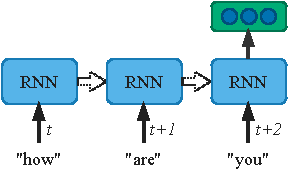
\includegraphics[width=6cm]{graphics/rnn}
      \caption{A recurrent neural network (RNN) consumes at each timestep one input word. Then, it produces a single vector representation of the inputs.}
      \label{fig:RNN}
    \end{figure}
    A common downside of RNNs is that they ``forget'' over longer sequences. This issue is addressed by introducing learnable \textit{gates}, an idea which soon led to a recurrent model called the Long Short-Term Memory network (LSTM) \citep{Hochreiter_Schmidhuber_1997}. An LSTM unit has a memory cell and learns to selectively add parts of the input into the memory, forget parts of the memory, and output parts of it (see \autoref{fig:rnn-lstm}). Long after being proposed in 1997, LSTMs gained popularity in NLP -- especially in text processing (see e.g. \citet{Mikolov_2010} and \citet{Graves_2013}). 
    \begin{figure}[h!t]
      \centering
      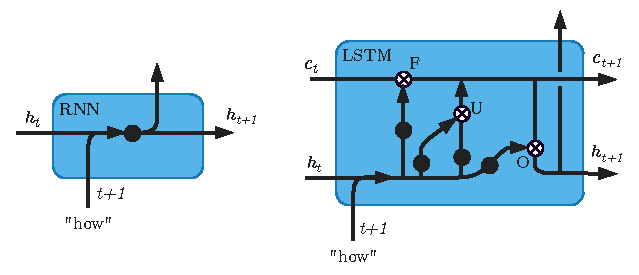
\includegraphics[width=13cm]{graphics/rnn-lstm}
      \caption{Comparing the internals of a vanilla RNN and an LSTM. The latter has three gates (shown as $\bigotimes$) -- the forget gate $F$, the update gate $U$, and the output gate $O$. $\bm{h}$ is the internal (hidden) state which can be used as the output at any timestep, $\bm{c}$ is the memory cell. With $\CIRCLE$ is shown a learnable non-linear transformation.}
      \label{fig:rnn-lstm}
    \end{figure}

    % A major breakthrough came when \citet{Kalchbrenner_2013} and \citet{Sutskever_2014} developed the encoder-decoder architecture for machine translation and other sequence-to-sequence tasks such as paraphrasing or parsing.
    As various recurrent models started dominating NLP, one particularly influential architecture emerged, addressing tasks such as machine translation, where the output is a new sequence rather than a simple decision. This was the \textit{encoder-decoder} architecture (first described by \citet{Hinton_1994}, later re-introduced in the NLP context by \citet{Kalchbrenner_2013} and \citet{Sutskever_2014}), see \autoref{fig:encoder-decoder}. It uses a recurrent encoder to turn an input sentence into a single vector, and a recurrent decoder to generate an output sequence based on the vector.
    \begin{figure}[h!t]
      \centering
      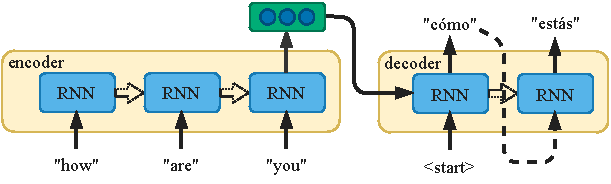
\includegraphics[width=11.5cm]{graphics/encoder-decoder}
      \cprotect\caption{An encoder-decoder model for machine translation. Notice how the decoder initially takes as input the special \verb|<start>| token and at later time consumes the previous output word.}
      \label{fig:encoder-decoder}
    \end{figure}

    % \citet{Bahdanau_2014} improved things by introducing attention, enabling the recurrent encoders to learn to selectively attend or ignore parts of the input sequence.
    \citet{Bahdanau_2014} improved encoder-decoder models by introducing the concept of \textit{attention}. The attention module helps the decoder produce better output by selectively focusing on the most relevant encoder hidden states at each decoder timestep. This is depicted in \autoref{fig:encoder-decoder-att}, showing the decoder just about to output the second word (``est\'as''). The steps (as numbered in the diagram) are:
    \begin{enumerate}
      \item the decoder's hidden state passed to the attention module,
      \item the intermediate hidden states of the encoder also passed to the attention module,
      \item the attention module, based on information from the decoder's state, selecting relevant information from the encoder's hidden states and combining it into the attentional \textit{context vector},
      \item the decoder combining the last output word (``c\'omo'') with the context vector and consuming this information to better decide which word to output next. 
    \end{enumerate}

    \begin{figure}[h!t]
      \centering
      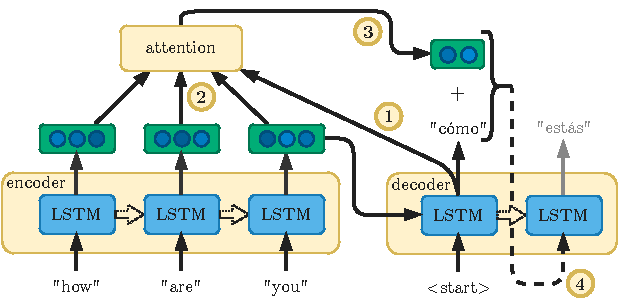
\includegraphics[width=11.5cm]{graphics/encoder-decoder-att}
      \cprotect\caption{An encoder-decoder model for machine translation with added attention mechanism.}
      \label{fig:encoder-decoder-att}
    \end{figure}
    
    The attention can be described more formally\footnote{My description does not exactly follow the original works of \citet{Bahdanau_2014} and \citet{Luong_2015}. Instead, I introduce concepts that will be useful in later sections of this work.}: First, the decoder state $\bm{h}_D$ is processed into a \textit{query} $\bm{q}$ using a learnable weight matrix $W_Q$:
    \begin{equation}
    \bm{q}=\bm{h}_DW_Q
    \end{equation}
    and each encoder state $\bm{h}_E^{(i)}$ ($i$ being the input position or encoder timestep) is used to produce the \textit{key} and \textit{value} vectors, $\bm{k^{(i)}}$ and $\bm{v^{(i)}}$:
    \begin{equation}
    \bm{k}^{(i)} = \bm{h}_E^{(i)}W_K,\ \ \ \bm{v}^{(i)} = \bm{h}_E^{(i)}W_V\ .
    \end{equation}
    Then, the selective focus of the attention is computed as an \textit{attention weight} $w^{(i)}$ for each input position \textit{i}, by combining the query with the $i$-th key:
    \begin{equation}
    w^{(i)}=\bm{q}^\top\bm{k}^{(i)}\ .
    \end{equation}
    The weights are normalised using softmax and used to create the context vector $c$ as a weighted average of the values:
    \begin{equation}
    \bm{c}=\sum_{i}a^{(i)}\bm{v}^{(i)}\ \ \ \textrm{where}\ \ \ a^{(i)}=\softmax(w^{(i)})=\frac{\exp{(w^{(i)})}}{\sum_{j}\exp{(w^{(j)})}}\ .
    \end{equation}
    Note that $W_Q$, $W_K$, $W_V$ are matrices of learnable parameters, optimised in training the model. This way, the attention's ``informed selectivity'' improves over time.
    
    For about 4 years, recurrent models with attention were the state of the art in many NLP tasks. However, as we will see, the potential of attention reached far beyond recurrent models.
  }

  \section{Transformer-based NLP}{
    \label{sec:Transformer-based-NLP}
    \subsection{Transformers}{
      \label{sec:Transformers}
      % \citet{Vaswani_2017} introduced Transformer. Main idea: process tokens in parallel, not sequentially, with sequentiality represented by positional markers (embeddings). Self-attention is used to pool from the context of the entire sequence, leading to evolving rich contextualised representations of each token in the higher layers.
      We saw how the attention mechanism can selectively focus on parts of a sequence to extract relevant information from it. This raises the question of whether processing the inputs in a sequential fashion with the recurrent encoder is still needed. In particular, RNN models are slow as a result of this sequentiality, and are hard to parallelise. In their influential work, \citet{Vaswani_2017} proposed an encoder-decoder model based solely on attention and fully parallelised: the \textit{Transformer}. The core element of the model is the \textit{self-attention} mechanism, used to process all input words in parallel.

      In particular, a Transformer model typically has multiple self-attention layers, each layer processing separate representations of all input words. Continuing with the three-word input example from \autoref{fig:encoder-decoder-att}, a high-level diagram of the workings of a self-attention layer is shown in \autoref{fig:self-att-layer}. Importantly, the input word representations evolve from lower to higher layers such that they consider not just the one input word, but also all other words -- the representation becomes \textit{contextual} (also referred to as a \textit{contextual embedding} of the word within the input sentence).

      \begin{figure}[h!t]
        \centering
        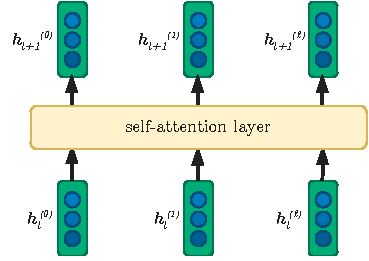
\includegraphics[width=8cm]{graphics/self-att-layer}
        \cprotect\caption{A high-level diagram of the application of self-attention in Transformer models. Three hidden states are shown for consistency with the length of the input shown in \autoref{fig:encoder-decoder-att}; in general, the input length can vary.}
        \label{fig:self-att-layer}
      \end{figure}

      As for the internals of self-attention, the basic principle is very similar to standard attention. Self-attention too is used to focus on and gather relevant information from a sequence of elements, given a query. However, to produce a richer contextual embedding $\bm{h}_{l+1}^{(i)}$ in layer $l+1$ of the $i$-th input word, self-attention uses the incoming representation $\bm{h}_l^{(i)}$ for the query, and considers focusing on all representations in layer $l$, including $\bm{h}_l^{(i)}$ itself. \autoref{fig:self-att} shows this in detail for input position $i=0$. Query $\bm{q}^{(0)}$ is produced and matched with every key in layer $l$ (i.e. $\bm{k}^{(0)},\ldots,\ \bm{k}^{(2)}$) to produce the attention weights. These weights quantify how relevant each representation $\bm{h}_l^{(i)}$ is with respect to position $i=0$. Then, the new contextual embedding $\bm{h}_{l+1}^{(i)}$ is constructed as a weighted sum of the values $\bm{v}^{(0)},\ldots,\ \bm{v}^{(2)}$ (same as constructing the context vector in standard attention).

      \begin{figure}[h!t]
        \centering
        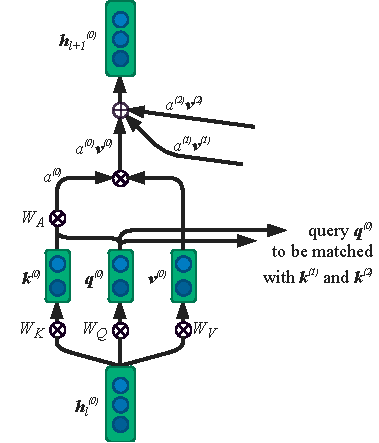
\includegraphics[width=12cm]{graphics/self-att}
        \cprotect\caption{The internals of self-attention, illustrated on creating the next-layer hidden representation of the input position $i=1$, given all representations in the current layer (previous, current, and following). Note that $\otimes$ stands for multiplication (where the multiplication involves a learnable matrix like $W_K$, this is written next to the $\otimes$), and $\oplus$ denotes summation.}
        \label{fig:self-att}
      \end{figure}

      % parallel nature
      Notice that, even though each contextual embedding considers all input positions, the next-layer contextual embeddings $\bm{h}_{l+1}^{(0)},\ldots,\ \bm{h}_{l+1}^{(2)}$ can be computed all at the same time, in parallel: First, the keys, queries and values for all input positions are computed; then, the attention weights with respect to each position are produced; finally, all the new representations are produced. It is this parallelism that allows Transformer models to run faster. As a result, they can be much bigger (and hence create richer input representations) than recurrent models while taking the same time to train.

      % positional embeddings
      Due to their parallel nature, self-attentional layers have no notion of an element's position within the input sequence. This means no sensitivity to word order. (Recurrent models sense this order quite naturally because they process input text word by word.) To alleviate this downside of self-attention, Transformers use \textit{positional embeddings}. These are artificially created numerical vectors added to each input word, different across input positions, thus enabling the model's layers to learn to be position- and order-sensitive.

      % multi-headedness
      As an additional improvement of the self-attentional mechanism, \citeauthor{Vaswani_2017} introduce the concept of multiple self-attention heads. This is very similar to having multiple instances of the self-attention module in \autoref{fig:self-att}, each instance being one \textit{head} and computing its own queries, keys and values. The motivation behind multiple self-attention heads is to enable each head $a$ to learn different ``focusing skills'' by learning its own $W_{Q,a}$, $W_{K,a}$, $W_{V,a}$. Each head produces its own output:
      \begin{equation}
      O_{att,a} = \softmax(\frac{\bm{q}\bm{k}^\top}{\sqrt{d_k}})\bm{v} = \softmax(\frac{(\bm{h}_l^\top{W_{Q,a}})^\top(\bm{h}_l^\top{W_{K,a}})}{\sqrt{d_k}})(\bm{h}_l^\top{W_{V,a}})
      \end{equation}
      which matches \autoref{fig:self-att} (but notice the detail of the additional scaling by $\frac{1}{\sqrt{d_k}}$, introduced by \citeauthor{Vaswani_2017}, where $d_k$ is the dimensionality of the key).
      The outputs of the $A$ individual attentional heads are then concatenated and dimensionality reduced with a trainable linear transformation $W_{AO}$, to produce the final output, which replaces $\bm{h_{l+1}}$ in \autoref{fig:self-att}:
      \begin{equation}
      O_{att} = [O_{att, 1},\ \ldots,\ O_{att, A}]W_{AO}\ .
      \end{equation}
      
      % \citet{Radford_2018} introduced the idea of generative LM pre-training and fine-tuning. This concept helps train much better models even for low-resource tasks with small datasets, by leveraging general language knowledge acquired by the model in the pre-training phase. Publishing pre-trained model instances makes the power of NLP much more accessible to anyone and has become a popular thing to do. (Also mention that subword tokens were used instead of words.)
      Besides the self-attention-based architecture, there is one more important property that makes today's Transformer models perform so well on a wide variety of NLP tasks: the way these models are trained. First used for Transformers by \citet{Radford_2018}\footnote{The idea was previously used with recurrent models by \citet{Dai_2015}.}, the general procedure is:
      \begin{enumerate}
        \item \textit{Unsupervised pre-training}: The model is trained on one or more tasks, typically language modelling, using huge training corpora. For example, \citeauthor{Radford_2018} pre-train their model to do next word prediction (the standard language modelling task) on a huge corpus of over 7,000 books.
        \item \textit{Supervised fine-tuning}: The pre-trained model is trained on a concrete dataset to perform a desired downstream task, such as predicting the sentiment of a sentence, translating between languages, etc.
      \end{enumerate}
      This two-step procedure is conceptually similar to using pre-trained word embeddings. In both cases, the aim is to learn general language knowledge and then use this as a starting point for focusing on a particular task. However, in this newer case, the word representations learned in pre-training are be better tailored to the specific architecture, and they are inherently contextual -- compared to pre-trained word embeddings like word2vec which are typically context-insensitive. 

      Importantly, pre-trained knowledge makes models more suitable for downstream tasks with limited amounts of labelled data. The model no longer needs to acquire all the desired knowledge just from the small dataset; it contains pre-trained high-quality general language knowledge which can be reused in various downstream tasks. This means that large, powerful Transformer models become more accessible: They are successfully applicable to a wider array of smaller tasks than large models that have to be trained from scratch.
    }

    \subsection{BERT}{
      \label{sec:BERT}
      % \citet{Devlin_2018} improved the concept by pre-training the model bi-directionally (leading to language modelling based on left \textit{and} right context).
      Perhaps the most popular Transformer model today is BERT (Bidirectional Encoder Representations from Transformers), proposed by \citet{Devlin_2018}. Architecturally, it is a sequence encoder, hence suited for sequence classification tasks. While being heavily based on the original Transformer \citep{Vaswani_2017}, BERT also utilises a number of further ideas:
      \begin{enumerate}
        \item The model learns bidirectional representations: It can be trained on language modelling that is not next-word prediction (prediction given left context), but word prediction given both the left and the right context.
        \item {It uses two very different pre-training classification tasks:
        \begin{enumerate}
          \item The \textit{masked language modelling} (MLM) task encourages BERT to learn good contextual word embeddings. The task itself is to correctly predict the token at a given position in a sentence, given that the model can see the entire sentence with the target token(s) masked out\footnote{I.e. replaced with the special \verb|[MASK]| token.}, with a different token, or left unchanged.
          \item The \textit{next-sentence prediction} (NSP) task encourages BERT to learn good sentence-level representations. Given two sentences, the task is to predict whether they formed a consecutive sentence pair in the text they came from, or not.
        \end{enumerate}
        The pre-training was carried out on text from books and from the English Wikipedia, totalling to 3,400 million words (for details see \citet{Devlin_2018}). The MLM and NSP tasks were both used throughout the pre-training, forcing the model to learn both at the same time.
        }
        \item The inputs are processed not word by word, but are broken down using a fixed vocabulary of sub-word units called \textit{wordpieces} (conceptually introduced by \citet{Sennrich_2016}, this particular variant created by \citet{Wu_2016}). This way, BERT can better deal with rare words -- by assembling them from pieces\footnote{In word-level models, words that are not found in the model's vocabulary are replaced with a special \verb|UNKNOWN| token, which means disregarding any information carried by the words.}. The tokeniser module of BERT uses the wordpiece vocabulary of \citeauthor{Wu_2016} to tokenise (segment) the input text before it is further processed. \autoref{fig:bert-inputs} shows an example; notice how my surname (``Sucik'') gets split into three wordpieces whereas the other, much more common words are found in the wordpiece vocabulary.
        \item To enable the different pre-training tasks as well as two-sentence inputs, BERT uses a special input sequence representation, illustrated in \autoref{fig:bert-inputs}. Given the two input sentences $S_A$, $S_B$, they are concatenated and separated by the special \verb|[SEP]| token. The overall sequence is prepended with the \verb|[CLS]| (classification) token. To explicitly capture that certain tokens belong to $S_A$ and others to $S_B$, simple \textit{token type embeddings} (which only take on two different values) are added to the token embedding at each position. Then, for tasks like NSP, only the output representation of the \verb|[CLS]| token (i.e. $\bm{o_0}$) is used, whereas for token-level tasks like MLM the output vector from the desired position is used (in \autoref{fig:bert-inputs}, the MLM task would use $\bm{o_3}$ to predict the correct token at this position).
      \end{enumerate}

      \begin{figure}[h!t]
        \centering
        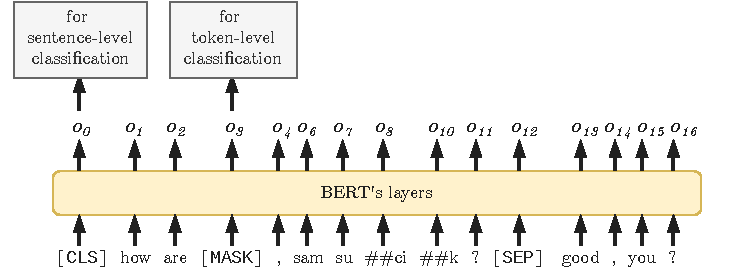
\includegraphics[width=14cm]{graphics/bert-inputs}
        \caption{BERT's handling of input for sentence-level and token-leven tasks. The input sentences ($S_A = How\ are\ you,\ Sam\ Sucik?$ and $S_B = Good,\ you?$) are shown as split by BERT's tokeniser, with the first instance of ``you'' masked out for MLM.}
        \label{fig:bert-inputs}
      \end{figure}
      % They also changed the pre-training to 2 tasks trained at the same time: masked language modelling to learn to understand words, and next sentence prediction to learn to reason about entire sentences (as the actual NLP tasks often require such reasoning). 
      % This is is how BERT was born, which then became extremely popular in the community, attracting a lot of work on improving it, analysing its capabilities, extending it to other languages, and even applying it to multi-modal tasks such as video captioning. 
      % TO-DO: elaborate more on BERT, also with a schematic picture.
      The overall architecture of BERT is shown in \autoref{fig:bert-hl}. The tokeniser also adds the special tokens like \verb|[CLS]| and \verb|[SEP]| to the input, while the trainable token embedding layer also adds the positional embedding and the token type embedding to the wordpiece embedding of each individual token. The pooler takes the appropriate model output (for sequence level classification the first output $\bm{o_0}$ as discussed above) and applies a fully-connected layer with the tanh activation function.
      The external classifier is often another fully-connected layer with the tanh activation, producing the logits\footnote{For a classifier, the logits are the (unnormalised) predicted class probabilities.}. These get normalised using softmax to produce a probability distribution over all classes. The most probable class get output as the model's prediction.
      
      \begin{figure}[h!t]
        \centering
        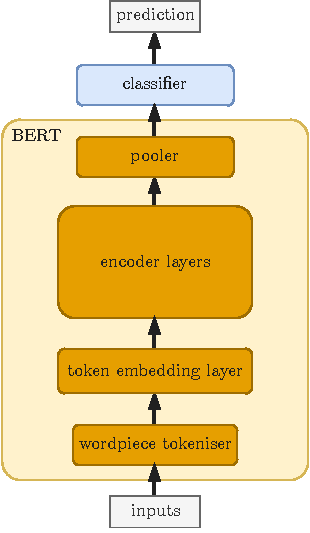
\includegraphics[width=6cm]{graphics/bert-hl}
        \caption{High-level overview of the modules that make up the architecture of BERT as used for sequence-level classification.}
        \label{fig:bert-hl}
      \end{figure}

      % things beyond what was said about Transformers already: residual connections, GeLU?
      To complete the picture of BERT, \autoref{fig:bert-encoder-layer} shows the internals of an encoder layer. Besides the multi-headed self-attention submodule, it also contains the fully-connected submodule. This uses a very wide intermediate fully-connected transformation with parameters $W_I$, inflating the representations up to the dimensionality $d_I$, and the layer output fully-connected transformation with parameters $W_O$, which reduces the dimensionality. Each submodule is also by-passed by a residual connection (shown with dashed lines). The residual information is summed with the submodule's output, and layer normalisation is applied to the sum. Note that this structure is not new in BERT; it was used already by the original Transformer of \citet{Vaswani_2017}. Conveniently, Transformers are designed such that all of the intermediate representations (especially the encoder inputs and outputs, and the self-attention layer inputs and outputs) have the same dimensionality $d_h$ -- this makes any residual by-passing and summing easy.

      \begin{figure}[h!t]
        \centering
        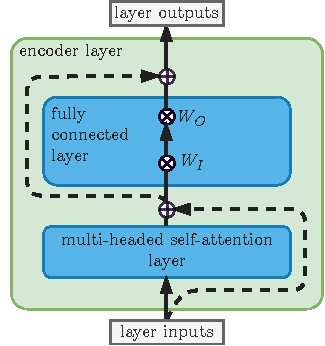
\includegraphics[width=6cm]{graphics/bert-encoder-layer}
        \caption{The modules making up one encoder layer in BERT; residual connections highlighted by using dashed lines. $\bigotimes$ marks learnable neural layers, $\bigoplus$ marks summation (in this case used to combine residual information with layer outputs).}
        \label{fig:bert-encoder-layer}
      \end{figure}

      When training BERT, artificial, intentional corruption of internal representations is done using dropout, which acts as a regulariser, making the training more robust. In particular, dropout is applied to the outputs of the embedding layer, to the computed attention weights, just before residual summation both to the self-attention layer output and to the fully connected layer output (see \autoref{fig:bert-encoder-layer} for the summation points), and to the output of the pooler module (before aplying the external classifier, see \autoref{fig:bert-hl}). The typical dropout rate used is 0.1.
      
      For updating the learnable parameters during training, BERT uses the popular Adam learning algorithm \citep{Kingma_2014}, which combines two main ideas:
      \begin{enumerate}
        \item \textit{Adaptive learning rates}, meaning that each learnable model parameter can have its own ``pace of learning''. In Adam, this individual pace is based on the observed recent gradients of the overall model error with respect to the single parameter.
        \item \textit{Momentum}, a mechanism used to deal with complex, stochastic error surfaces, by preferring only that direction in the parameter space, which leads to stable improvements (and dispreferring directions which only result in short-term, stochastic improvements). Two decay rates $\beta_1$ and $\beta_2$ realise the momentum -- they control how quickly and noisily or slowly and smoothly the adaptation of the learning rate happens. In practice, the high values $\beta_1=0.9$ and $\beta_2=0.999$ are often used (as recommended by \citeauthor{Kingma_2014}), meaning relatively slow and smooth adaptation.
      \end{enumerate}
      
      Originally, pre-trained BERT was released in two sizes: BERT\textsubscript{Base} with 110 million parameters, 12 encoder layers and 12-head self-attention, and BERT\textsubscript{Large} with 340 million parameters, 24 encoder layers and 16-head self-attention. The models quickly became popular, successfully applied to various tasks from document classification \citep{Adhikari_2019} to video captioning \citep{Sun_2019}. Further pre-trained versions were released too, covering, for example, the specific domain of biomedical text \citep{Lee_2019} or multilingual text \citep{Pires_2019}.
    }

    \subsection{Newer and larger Transformer models}{
      \label{sec:post-BERT-models}
      % Following the success of BERT, further and often bigger Transformer models started emerging:
      Following the success of the early Transformers and BERT \citep{Vaswani_2017,Radford_2018,Devlin_2018}, many further model variants started emerging, including:
      \begin{itemize}
        \item The OpenAI team releasing GPT-2 \citep{Radford_2019}, a larger and improved version of their original, simple Transformer model GPT \citep{Radford_2018}.
        \item \citet{Lample_2019} introducing XLM, which uses cross-lingual pre-training and is thus better suited for downstream tasks in different languages.
        \item Transformer-XL \citep{Dai_2019}, which features an improved self-attention that can handle very long contexts (across multiple sentences/documents).
      \end{itemize}

      All these open-sourced, powerful pre-trained models were a significant step towards more accessible high-quality NLP (in the context of downstream tasks with limited data). However, the model size -- often in 100s of million trainable parameters -- meant these models could not be applied easily in practice (outside of research): They were memory-hungry and slow.
      
      Naturally, this inspired another stream of research: Compressing large, well-performing Transformer models (very often BERT) to make them faster and resource-efficient.
      I turn my focus to one compression method that worked particularly well so far: the teacher-student knowledge distillation.
    }
  }

  \section{Teacher-student knowledge distillation}{
    \label{sec:KD}
    % brief history of KD in general
    % different objectives: logits, hard labels, mimicking internal representations...
    \subsection{A brief introduction to knowledge distillation}{
      \label{sec:KD-intro}
      Knowledge distillation was introduced by \citep{Bucila_2006} as a way of knowledge transfer from large models into small ones. The aim is to end up with a smaller -- and hence faster -- yet well-performing model. The steps are 1) to train a big neural classifier model (also called the \textit{teacher}), 2) to let a smaller neural classifier model (the \textit{student}) learn from it -- by learning to mimic the teacher's behaviour. Hence also the name \textit{teacher-student knowledge distillation}, often simply \textit{knowledge distillation}.
      
      There are different ways of defining the teacher's ``behaviour'' which the student learns to mimic. Originally, this was realised as learning to mimic the teacher's predictions: A dataset would be labelled by the teacher, and the student would be trained on these labels (which are in this context referred to as the \textit{hard labels}). The dataset used for training the student (together with the teacher-generated labels) is referred to as the \textit{transfer dataset}.

      Later, \citet{Ba_2013} introduced the idea of learning from the teacher-generated \textit{soft labels}, which are the teacher's logits. The idea is to provide the student with richer information about the teacher's decisions: While hard labels only express which class had the highest predicted probability, soft labels also describe how confident the prediction was and which other classes (and to what extent) the teacher was considering for a given example.

      When soft labels were first used, the student's training loss function was the mean squared distance between the student's and the teacher's logits:
      \begin{equation}
        E_{MSE}=\sum_{c=1}^{C}{(z_t^{(c)}-z_s^{(c)})^2}
        \label{eq:E_MSE}        
      \end{equation}
      where $C$ is the number of classes and $z_t$, $z_s$ are the the teacher's and student's logits.
      \citet{Hinton_2015} proposed a more general approach, addressing the issue of overconfident teachers with very sharp logit distributions. The issue with such distributions is that they carry little additional information beyond the hard label (since the winning class has a huge probability and all others have negligibly small probabilities).
      To ``soften'' such sharp distributions, \citeauthor{Hinton_2015} proposed using the \textit{cross-entropy loss} \autoref{eq:E_CE} in combination with \textit{softmax with temperature} \autoref{eq:softmax-temperature} (instead of the standard softmax) in training both the teacher and the student.
      \begin{equation}
        E_{CE}=\sum_{c=1}^{C}{z_t^{(c)} \log{z_s^{(c)}}}
        \label{eq:E_CE}        
      \end{equation}
      \begin{equation}
        p_c=\frac{\exp{(z^{(c)}/T})}{\sum_{c'=1}^{C}{\exp{(z^{(c')}/T)}}}
        \label{eq:softmax-temperature}        
      \end{equation}
      The temperature parameter $T$ determines the extent to which the distribution will be ``unsharpened'' -- two extremes being the completely flat, uniform distribution (for $T \rightarrow \infty$) and the maximally sharp distribution\footnote{I.e. having the preferred class's probability 1 and the other classes' probabilities 0.} (for $T \rightarrow 0$). When $T > 1$, the distribution gets softened and the student can extract richer information from it. Today, using soft labels with the cross-entropy loss with temperature is what many refer to simply as knowledge distillation.

      Since 2015, further knowledge distillation variants have been proposed, enhancing the vanilla technique in various ways, for example:
      \begin{itemize}
        \item \citet[p. 13]{Papamakarios_2015} points out that mimicking teacher outputs can be extended to mimicking mimicking the \textit{derivatives} of the teacher's loss with respect to the inputs. This is realised by including in the student's loss function also the term: $\frac{\partial \bm{o}_s}{\partial \bm{x}} - \frac{\partial \bm{o}_t}{\partial \bm{x}}$ ($\bm{x}$ being an input, e.g. a sentence, and $\bm{o}$ being the output, e.g. the predicted class). %, the additional loss term being calculated using the R technique (Pearlmutter, 1994).
        \item \citet{Romero_2015} proposed to additionally match the teacher's internal, intermediate representations of the input. \citet{Huang_2017} achieved this by learning to align the distributions of neuron selectivity patterns between the teacher's and the student's hidden layers. Unlike standard knowledge distillation, this approach is no longer limited only to classifier models with softmax outputs (see the approach of \citet{Hinton_2015} discussed above).
        \item \citet{Sau_2016} showed that learning can be more effective when noise is added to the teacher logits.
        \item \citet{Mirzadeh_2019} showed that when the teacher is much larger than the student, knowledge distillation performs poorly, and improved on this by ``multi-stage'' distillation: First, knowledge is distilled from the teacher into an intermediate-size ``teacher assistant'' model, then from the assistant into the final student.
      \end{itemize}
    }

    \subsection{Knowledge distillation in NLP}{
      \label{sec:kd-nlp}
      % \citet{Kim_2016} observe that KD and weight pruning are orthogonal (can be used together), and that mimicking top-most hidden layer outputs (instead of outputs themselves) doesn't provide improvements previously reported.
      % Practically all the so far mentioned research in knowledge distillation was done in the domain of image processing. This comes as no surprise: It was image processing that was benefitting the most from the resurgence of deep learning. Ever since the AlexNet \citep{Krizhevsky_2012}, bigger and bigger models were proposed, simultaneously driving the research in model compression so as to make the models usable in practice.
      The knowledge distillation research discussed so far was tied to the image processing domain. This is not surprising: Image processing was the first area to start taking advantage of deep learning, and bigger and bigger models had been researched ever since the revolutional AlexNet \citep{Krizhevsky_2012}.

      % KD in NLP: sequence-level KD \citep{Kim_2016}, then basically straight to distilling from BERT?
        % In the NLP literature, it has previously been used in neural machine translation (Kim and Rush, 2016) and language modeling (Yu et al., 2018).
      % In natural language processing, research on knowledge distillation was rare for a long time. One notable work was the adaptation of distillation for sequence-to-sequence machine translation models -- whose outputs are no longer simple classification scores -- by \citet{Kim_2016}. Another pioneering study compressed a recurrent neural language model for use on mobile devices \citep{Yu_2018}.
      In NLP and in text processing in particular, the (recurrent) models were moderately sized for a long time, not attracting much research in model compression. Still, one early notable work was on adapting knowledge distillation for sequence-to-sequence models \citep{Kim_2016}, while another pioneering study \citep{Yu_2018} distilled a recurrent model into an even smaller one -- to make it suitable for running on mobile devices.

      Understandably, the real need for model compression started very recently, when the large pre-trained Transformer models became popular. Large size and low speed seemed to be the only downside of these -- otherwise very successful and accessible -- models.

      % When distilling knowledge from big, pre-trained Transformer models, the main decision is whether to distil before or after fine-tuning on a concrete downstream task. Each option has its pros and cons.
      Perhaps the first decision to make when distilling large pre-trained models is at which point to distill. In particular, one can distill the general knowledge from a pre-trained teacher and use such a general student by fine-tuning it on downstream tasks, or one can fine-tune the pre-trained teacher on a task and then distill this specialised knowledge into a student model meant for the one task only. Each of these approaches has its advantages and disadvantages.

      In the first scenario (distilling pre-trained knowledge), a major advantage is that the distillation happens once and the small student can be fine-tuned quickly for various downstream tasks.
      Since the distillation can be done on the same data that the teacher was pre-trained on -- large unlabelled text corpora --, lack of transfer data is not a concern.
      A possible risk is that the large amount of general pre-trained language knowledge will not ``fit'' into the small student, requiring the student itself to be relatively large. \citet{Sanh_2019} took this approach and, while their student is successfully fine-tuned for a wide range of tasks, it is only 40\% smaller than the BERT\textsubscript{Base} teacher.

      % Distilling beforeinto a small student and subsequently finetuning it on any downstream task means easy 
      %   pros: have flexible model that's easy to finetune for any downstream task. lots of transfer data to work with.
      %   cons: too small model may not be able to take all of teacher's useful knowledge
      %   Sanh tried and only got to making BERT 60\% smaller??? (# of params).

      % CAREFUL NOT TO MIX IN OWN METHODOLOGY HERE!!!
      In the second scenario, only the task-specific knowledge needs to be transferred to the student -- potentially allowing smaller students.
      However, teacher fine-tuning and distillation have to be done anew for each task and this is resource-hungry.
      Additionally, there may be a lack of transfer data if the downstream task dataset is small.
      Various ways of addressing this issue by \textit{augmenting} small datasets have been proposed, with mixed success. 
      \citet{Mukherjee_2019} use additional unlabelled in-domain sentences with labels generated by the teacher -- this is limited to cases where such in-domain data are available. \citet{Tang_2019a} create additional sentences using simple, rule-based perturbation of existing sentences from the downstream dataset. Finally, \citet{Jiao_2019} and \citet{Tang_2019b} use large Transformer models generatively to create new sentences. In the first case, BERT is applied repeatedly to an existing sentence, changing words into different ones one by one and thus generating a new sentence. In the second case, new sentences are sampled token-by-token from a GPT-2 model fine-tuned on the downstream dataset with the next-token-prediction objective.
      % After:
      %   pros: only task-specific knowledge is distilled, likely into much smaller model.
      %   cons: have to train big teacher for each downstream task, likely to take long. may need more transfer data than small downstream dataset.
      %   Tang: distilled into much smaller student. didn't address issue of having to train teacher repeatedly. addressed issue of little data quite successfully.

      % In this work, I adopt the approach of \citet{Tang_2019b} as I view it as the most promising one so far. However, while they use only bidirectional LSTM students, I also experiment with a smaller version of BERT, similarly to \citet{Jiao_2019}. For detailed description of the system see \autoref{chap:implementation}.
      Clearly, each approach is preferred in a different situation: If the requirement is to compress the model as much as possible, and there is enough transfer data, distilling the fine-tuned teacher is more promising. If, on the other hand, one wants to make available a re-usable, small model, then distilling the broader, pre-trained knowledge is preferred.
    }
  }
  
  \section{Interpreting NLP models}{
    \label{sec:understanding-models}
    % NNs are black boxes and (not) understanding the models is a serious issue.
    Neural models are by their very nature opaque or even black boxes, and (not) really understanding the models is a serious concern.
    % performance is typically more important than transparence, but recently the demand for explainable AI (XAI) has been increasing. additionally, understanding is opportunity for further improvements of the mdels and techniques.
    Despite the typical preferrence of performance over transparence, recently, the demand for explainable artificial intelligence (XAI) has been increasing, as neural models become widely used. (Besides the DARPA XAI program\footnote{\rurl{www.darpa.mil/program/explainable-artificial-intelligence}}, conferences like the International Joint Conference on Artificial Intelligence (IJCAI), the SIGKDD Conference on Knowledge Discovery and Data Mining (KDD), and the Conference on Computer Vision and Pattern Recognition (CVPR) now feature dedicated XAI workshops\footnote{See \rurl{sites.google.com/view/xai2019/home}, \rurl{xai.kdd2019.a.intuit.com/}, \rurl{explainai.net/}.}.)

    % in image processing, interpretability is easy thanks to visualising things. (somewhat similarly music.) notable works: maximising activation, visualising neurons' output for given input, maximum activation samples.
    The area of image processing has seen the most attempts at interpreting neural models and their behaviour. One reason being that vision tasks are often doable and easy to reason about for researchers and for humans in general. Various techniques shed light into the behaviour of image classifiers; for instance, techniques for creating images that maximally excite certain neurons \citep{Simonyan_2013}, or highlighting those parts of an image that a particular neuron ``focuses'' on \citep{Zeiler_2013}. 
    
    In NLP, interpretation is more difficult. Additionally, most research in interpreting NLP models started only relatively recently, after large neural models became widely used.
    % hard to do maximising activation or visualising single units. BUT types of information preserved in internal input representations can be well explored: probing!
    In their review, \citet{Belinkov_2018} observe that many methods for analysing and interpreting models are simply adapted from image processing, in particular the approach of visualising a single neuron's focus, given an input.
    In attentional sequence-to-sequence models, the attention maps can be visualised to explore the soft alignments between input and output words (see, e.g., \citet{Strobelt_2018}). However, these methods are mostly qualitative and suitable for exploring individual input examples, thus not well suited for drawing statistically backed conclusions or for model comparison.
    
    More quantitative and NLP-specific are the approaches that explore the linguistic knowledge present in a model's internal representations.
    Most often, this is realised by \textit{probing} the representations for specific linguistic knowledge: trying to automatically recover from them specific properties of the input. When such recovery works well, the representations must have contained the linguistic knowledge tied to the input property in question.
    First used by \citet{Shi_2016} for exploring syntactic knowledge captured by machine translation models, this general approach was quickly adopted more widely.
    \citet{Adi_2017} explored sentence encodings from recurrent models by probing for simple properties like sentence length, word content and word order.
    More recently, \citet{Conneau_2018} curated a set of 10 probing tasks ranging from easy surface properties (e.g. sentence length) through syntactic (e.g. the depth of the syntactic parse tree) to semantic ones (e.g. identifying semantically disrupted sentences).
    Focusing on Transformers, \citet{Tenney_2019a} proposed a set of \textit{edge probing} tasks, examining how much contextual knowledge about an entire input sentence is captured within the contextual representation of one of its words.
    Their tasks correspond to the typical steps of a text processing pipeline -- from part-of-speech (POS) tagging to identifying dependencies and entities to semantic role labelling. 
    \citet{Tenney_2019b} managed to localise the layers of BERT most important for each of these ``skills''. They showed that the ordering of these ``centres of expertise'' within BERT's encoder matches the usual low- to high-level order: from simple POS tagging in the earlier layers to more complex semantic tasks in the last layers.

    While the discussed approaches provide valuable insights, they merely help us intuitively describe or quantify the kinds of internal knowledge/expertise present in the models. 
    \citet{Gilpin_2018} call this level of model understanding \textit{interpretability} -- comprehending what a model does. 
    However, they argue that what we should strive to achieve is \textit{explainability}: the ability to ``summarize the reasons for neural network behavior, gain the trust of users, or produce insights about the causes of their decisions''.
    In this sense, today's methods achieve only interpretability because they enable researchers to describe but not explain -- especially in terms of causality -- the internals and decisions of the models.
    Still, interpreting models is an important step not only towards explaining them, but also towards understanding the properties of different architectures and methods and improving them.
    
    % In this work, I also attempt to mainly \textit{interpret} the student and teacher models. I adopt two approaches:
    % \begin{enumerate}
    %   \item analysing the mistakes the models make on the downstream task they were trained to do, including how confident the correct and incorrect predictions are
    %   \item probing the models using the probing tasks curated by \citet{Conneau_2018}
    % \end{enumerate}
    % By comparing the findings between models trained on different downstream tasks or with different architectures, I try to characterise each task in terms of the linguistic capabilities it utilises. 
    % Further, I describe how different student model architectures influence how linguistic knowledge is distilled from a teacher and stored in the student, and what the effect on the student's confidence is. 
    % Finally, I try to relate the observed effects to the method of knowledge distillation itself.
  }

  \section{Conclusions \reviewready}{
    % deep neural models widely used in NLP
    Since around 2013, the area of NLP has been taking advantage of deep neural models.
    % recently even larger Transformer models -- accessible but slow
    With the introduction of Transformers, the models became even deeper and more powerful.
    Today's pre-trained Transformer-based models like BERT make state-of-the-art NLP relatively accessible, but the models are often too large and slow for practical applications.
    % compression (KD) revival
    Compressing such models has become an active research area, with knowledge distillation being a particularly successful compression technique.
    % better understanding of new models as well as techniques desired
    However, the self-attentional, Transformer-based models, as well as compressing them, are still relatively young concepts.
    More research is needed to better interpret the behaviour of models like BERT, and to better understand the nature of the knowledge transfer from large Transformers into smaller, compressed ones.
  }
}

\chapter{Datasets \reviewed}{
  \label{chap:datasets}

  In this chapter, I introduce the different datasets used throughout the work:
  \begin{enumerate}
    \item To later experiment with models in the context of a wide range of NLP tasks, I use different small \textbf{downstream task datasets} on which I train large Transformer models.
    \item For knowledge distillation from the large into smaller models, large \textbf{transfer datasets} are used, created from the downstream datasets using data augmentation.
    \item Finally, \textbf{probing datasets} are used for analysing the linguistic capabilities of the large and the small models.
  \end{enumerate}

  \section{Downstream tasks}{
    The downstream task datasets I use to fine-tune the teacher model. The tasks are chosen to be diverse so that the knowledge distillation analysis later in this work is set in a wide NLP context. At the same time, all the datasets are rather small and therefore well representing the type of use case where pre-trained models like BERT are desirable due to the lack of labelled fine-tuning data.

    Today, perhaps the most widely used collection of challenging NLP tasks\footnote{Challenging by the nature of the tasks and by the small dataset size.} is the GLUE benchmarking collection \citep{Wang_2018}.
    This collection comprises 11 tasks which enable model benchmarking on a wide range of NLP tasks from sentiment analysis to detecting textual similarity, all framed as single-sentence or sentence-pair classification.
    Each task comes with an official scoring metric (such as accuracy or F1), labelled training and evaluation datasets, and a testing dataset with labels not released publicly.
    The test-set score accumulated over all 11 tasks forms the basis for the popular GLUE leaderboard\footnote{\rurl{gluebenchmark.com/leaderboard}}.
    
    In this work, I use single-sentence classification tasks (i.e. not sentence-pair tasks). Therefore, only two GLUE tasks are suitable for my purposes -- the Corpus of Linguistic Acceptability (CoLA) and the Stanford Sentiment Treebank in its binary classification variant (SST-2). 
    Additionally, I choose a third task to make my work cover the area of conversational language. This way, I build on my previous research in compressing BERT for conversational tasks \citet{Sucik_2019}, undertaken as part of an internship with Rasa\footnote{\rurl{rasa.com}}, a company building open-source tools for conversational AI. The third dataset, called Sara, focuses on classifying human messages from human-bot conversations according to their intent.

    \subsection{Corpus of Linguistic Acceptability}{
      \label{sec:datasets-CoLA}

      The CoLA dataset \citep{CoLA-paper} comprises roughly 8,500 training sentences, 1,000 evaluation and 1,000 testing sentences.
      The task is to predict whether a given sentence represents acceptable English or not (binary classification).
      All the sentences are collected from linguistic literature where they were originally hand-crafted to demonstrate various linguistic principles and their violations.
      
      The enormous variety of principles, together with many hand-crafted sentences that comply with or violate a principle in a niche way, make this dataset very challenging even for the state-of-the-art Transformer models. 
      As a non-native speaker, I myself struggle with some of the sentences, for instance:
      \begin{itemize}
        \item \textit{*The car honked down the road.} (unacceptable\footnote{The ``*'' is a standard way to mark ungrammatical sentences in linguistic literature.})
        \item \textit{Us, we'll go together.} (acceptable)
      \end{itemize}

      There are many examples which are easy for humans to classify but may be challenging for models which have imperfect understanding of the real world. Sentences like ``Mary revealed himself to John.'' require the model to understand that ``Mary'', being a typical female name, disagrees with the masculine ``himself''.
      
      The scoring metric is Matthew's Correlation Coefficient (MCC) \citep{Matthews_1975}, a correlation measure between two binary classifications. The coefficient is also designed to be robust against class imbalance, which is important because the dataset contains many more acceptable examples than unacceptable ones.
    }

    \subsection{Stanford Sentiment Treebank}{
      \label{sec:datasets-SST-2}

      The SST-2 dataset \citep{SST-paper} is considerably bigger than CoLA, with roughly 67,000 training examples, 900 evaluation and 1,800 testing examples. It contains sentences and phrases from movie reviews collected on \rurl{rottentomatoes.com}. The main SST dataset comes with human-created sentiment annotations on the continuous scale from very negative to very positive. SST-2 is a simplified version with neutral-sentiment phrases removed, only containing binary sentiment labels (positive and negative).

      Unlike the hand-crafted examples in CoLA, many examples in SST-2 are not the best-quality examples. In particular, sentences are sometimes split into somewhat arbitrary segments\footnote{This is due to the use of an automated parser in creating the dataset.}, such as:
      \begin{itemize}
        \item \textit{should have been someone else - } (negative)
        \item \textit{but it could have been worse.} (negative)
      \end{itemize}
      
      The labels are also sometimes unclear, see:
      \begin{itemize}
        \item \textit{american chai encourages rueful laughter at stereotypes only an indian-american would recognize.} (negative)
        \item \textit{you won't like roger, but you will quickly recognize him.} (negative)
      \end{itemize}

      Despite the problematic examples, most are straightforward (e.g. ``delightfully cheeky'' or ``with little logic or continuity''), making this task a relatively easy one. With accuracy being the official metric, best models in the GLUE leaderboard score over 97\%, very close to the official human baseline of 97.8\%\footnote{See the GLUE leaderboard at \rurl{gluebenchmark.com/leaderboard}}.
    }

    \subsection{Sara \reviewready}{
      \label{sec:datasets-Sara}

      As the third task, I use an intent classification dataset created by Rasa, a start-up building open-source tools for conversational AI\footnote{For transparency: My co-supervisor for this work -- Vladimir Vlasov -- is a Rasa employee, and he also supervised me during my Machine learning research internship with Rasa in the summer of 2019.}.

      The dataset is named Sara after the chatbot deployed on the company's website\footnote{See the bot in action at \rurl{rasa.com/docs/getting-started/}.}
      The Sara chatbot is aimed for holding conversations with the website visitors on various topics, primarily answering common questions about Rasa and the tools that it develops (the same tools were used to build Sara).
      To support diverse topics, Sara internally classifies each human message as one of 57 intents and then generates an appropriate response. The Sara dataset is a collection of human-generated message examples for each of the 57 intents, e.g.:
      \begin{itemize}
        \item \textit{what's the weather like where you are?} (ask\_weather)
        \item \textit{what is rasa actually} (ask\_whatisrasa)
        \item \textit{yes please!} (affirm)
        \item \textit{i need help setting up} (install\_rasa)
        \item \textit{where is mexico?} (out\_of\_scope)
      \end{itemize}
      \textit{For a list of all intents, explained and accompanied with real examples from the dataset, see \autoref{tab:sara-intent-list} in \autoref{chap:A-Sara}.}

      In the early days of the chatbot, it supported fewer intents, and several artificial examples per intent were first hand-crafted by Rasa employees to train the initial version of Sara's intent classifier. After Sara was deployed, more examples were collected and annotated from conversations with the website's visitors\footnote{To get a consent for such use of the conversations, each visitor was shown the following before starting a conversation with Sara: ``Hi, I'm Sara! By chatting to me you agree to our privacy policy.'', with a link to \rurl{rasa.com/privacy-policy/}}. Inspired by the topics that people tended to ask about, new intent categories were added. Today, the dataset still evolves and can be found -- together with the implementation of Sara -- at \rurl{github.com/RasaHQ/rasa-demo} (accessed April 3, 2020). It contains both the original hand-crafted examples as well as the (much more abundant) ``real'' examples.

      The Sara dataset version I use dates back to October 2019, when I obtained it from Rasa and pseudonymised the data\footnote{As a former employee of Rasa, I got access to the data under the NDA I had signed with the company. I had a permission from Rasa to use the pseudonymised data for this project; the use complied with the ethical approval process of Rasa.}. In particular, I removed any names of persons and e-mail addresses in any of the examples, replacing them with the special tokens \verb|__PERSON_NAME__| and \verb|__EMAIL_ADDRESS__|, respectively.      
      The dataset comprises roughly 4,800 examples overall, and was originally split into 1,000 testing examples and 3,800 training examples. 
      I further split the training partition into training and evaluation, with roughly 2,800 and 1,000 examples, respectively. All three partitions have the same class distribution.

      In line with how the dataset is used for research at Rasa, I use as the main scoring metric the multi-class micro-averaged F1 score ($\text{F1}_{micro}$), even though other reasonable metrics exist. First of all, in the binary classification case, the F1 score balances two desirable properties of any classifier: precision $P$ and recall $R$: $\text{F1} = \frac{2 P R}{P+R}$.
      $P$ quantifies the purity of reported positives: $P=TP/(TP+FP)$, $R$ quantifies the reported portion of all positives: $R=TP/(TP+FN)$ (where $TP$ are true positives, $FP$ are false positives, and $FN$ are false negatives).
      In classification with more than 2 classes, one can still compute the F1 score with respect to each individual class (treating the multi-class classification as a collection of binary classification decisions). Taking the average of such class-specific F1 scores leads to the \textit{macro-averaged} F1 metric:
      \begin{equation}
        \text{F1}_{macro} = \frac{1}{C}\sum_c \text{F1}_c = \frac{1}{C}\sum_c \frac{2 P_c R_c}{P_c+R_c}, \ \  C\ \text{being the number of classes}
      \end{equation}
      While this metric quantifies the F1 score on an ``average'' class, it does not account for different class sizes. In particular, if there are many small classes with little data and hence low F1 scores, then the average F1 will be pulled down -- even if the classifier succeeds on most data, which belongs to several big classes.
      One way to deal with these undesirable effects of class imbalance is to use the \textit{micro-averaged} F1 score. As its name suggest, it can be thought of as F1 averaged not on the macro level (classes), but on the micro level (individual examples), where the F1 score for a single example is 1 for a correct prediction (this follows from the standard formula $\text{F1} = \frac{2 P R}{P+R}$) and 0 for an incorrect prediction (by definition):
      \begin{equation}
        \text{F1}_{micro} = \frac{1}{N}\sum_n \text{F1}_n = \frac{1}{N}\sum_n {\begin{cases}\text{if correct} & 1\\ \text{else} & 0\end{cases}}\ ,\ \ \  N\ \text{being the number of examples}
      \end{equation}
      This score does take into account class imbalance because each example has ``one vote'' in the averaging process. Therefore, it is well suited for situations where the classifier should perform well on many examples, not necessarilly on many classes (as there can be many classes that are insignificant).
      Additionally, the $\text{F1}_{micro}$ score has the same value as accuracy.
    }
  }

  \section{Data augmentation for larger transfer datasets}{
    \label{sec:augmentation}
    As discussed in \autoref{sec:kd-nlp}, knowledge distillation works best with large amounts of data used as the transfer datasets. When the transfer dataset is small, it does not provide enough opportunity for the teacher to ``demonstrate its knowledge'' to the student, and the student learns little. Therefore, for each downstream task, I create a large transfer dataset by ``inflating'' the small training portion of the corresponding downstream dataset -- by augmenting it with additional sentences. I then add teacher logits to such augmented dataset, and use it to train the student models.

    \citet{Tang_2019b} demonstrated on several GLUE tasks that using an augmented training portion for distillation leads to much better student performance than using just the original small training portion.
    For CoLA in particular, using just the small original training set led to very poor student performance (see Table~1 in \citeauthor{Tang_2019b}).
    
    I take the augmentation approach that \citeauthor{Tang_2019b} found to work the best: Generating additional sentences using a GPT-2 model \citep{Radford_2019} fine-tuned on the training set\footnote{I used the code for \citet{Tang_2019b} which is available at \rurl{github.com/castorini/d-bert} (accessed April 4, 2020).}. The steps for creating the transfer dataset from the training portion are:
    \begin{enumerate}
      \item Fine-tune the pre-trained GPT-2 model (the 345-million-parameter version) on the training portion for 1 epoch (where an epoch is one complete pass through all training examples) with the language-modelling objective (i.e. predicting the next subword token given the sequence of tokens so far).
      \item Sample from the model a large number of tokens to be used as the beginnings (\textit{prefixes}) of the augmentation sentences. This sampling can be done as one-step next-token prediction given the special \verb|SOS| (start-of-sentence) token.
      \item Starting from each sampled prefix, generate an entire sentence token by token by repeatedly predicting the next token using the GPT-2 model. The generation of a sentence stops when the special \verb|EOS| (end-of-sentence) token is generated or when the desired maximum sequence length is reached (in this case 128 tokens).
      \item Add the generated augmentation sentences to the original training data, and generate the teacher logits for each sentence.
    \end{enumerate}

    For consistency with \citet{Tang_2019b}, I added 800,000 augmentation sentences to the training data of each of the three downstream tasks, resulting in the transfer datasets comprising roughly 808,500, 867,000, and 802,800 sentences for CoLA, SST-2, and Sara, respectively.
  }

  \section{Probing tasks}{
    The probing tasks (discussed in \autoref{sec:understanding-models}) I use after knowledge distillation to analyse the linguistic capabilities of the students and the teacher. In particular, I use the probing suite curated by \citet{Conneau_2018}, consisting of 10 tasks\footnote{The data, along with code for probing neural models, are publicly available as part of the SentEval toolkit for evaluating sentence representations \citep{SentEval-paper} at \rurl{github.com/facebookresearch/SentEval} (accessed April 4, 2020).}.

    \begin{figure}[h!t]
      \centering
      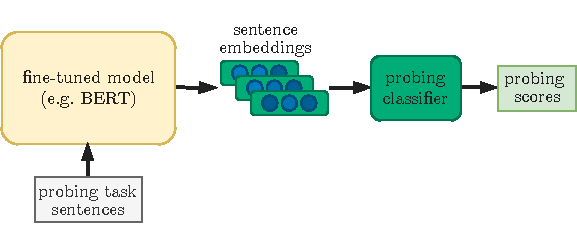
\includegraphics[width=11cm]{graphics/probing-scheme}
      \caption{A high-level diagram of the probing process.}
      \label{fig:probing-scheme}
    \end{figure}

    Each probing task is a collection of 120,000 labelled sentences, split into training (100,000), evaluation (10,000) and test (10,000) set. The label refers to a property of the sentence, such as the sentence's length. The aim is to recover the property from an encoding of the sentence, produced by the model being probed. \autoref{fig:probing-scheme} shows the basic workflow. First, the model is used to produce an encoding of each sentence. Then, a light-weight classifier is trained, taking the training sentences' encodings as inputs and learning to produce the labels. The evaluation sentence encodings are used to optimise the hyperparameters of the classifier. Finally, a probing score (accuracy) is produced on the test encodings. The score quantifies how well the sentence property in question is recoverable (and thus present) in the encodings. This serves as a proxy measure of the linguistic knowledge tied to the property. If, for instance, the property to be recovered is the depth of a sentence's syntactic parse tree, the score hints at the model's (un)capability to understand (and parse) the syntax of input sentences.
    By extracting probing encodings from different parts of a model (e.g. from different layers), the probing scores can additionally serve as cues for localising the linguistic knowledge in question -- one can observe how the amount of this knowledge varies across different model parts and where it is most concentrated.

    Regarding the linguistic capabilities explored by the probing suite, each task falls into one of three broad categories -- surface properties, syntax, and semantics:
    \begin{enumerate}
      \item {Surface information:
        \begin{itemize}
          \item \textbf{Length} is about recovering the length of the sentence. The labels are somewhat simplified: The actual sentence lengths grouped into 6 equal-width bins -- making this task a 6-way classification.
          \item \textbf{WordContent} is about identifying which words are present in the sentence. A collection of 1000 mid-frequency words was curated, and sentences were chosen such that each contains exactly one of these words. The task is identify which one (1000-way classification).
        \end{itemize}
      }
      \item{Syntactic information:
        \begin{itemize}
          \item \textbf{Depth} is about classifying sentences by their syntactic parse tree depth, with depths ranging from 5 to 12 (hence 8-way classification).
          \item \textbf{BigramShift} is about sensitivity to (un)natural word order -- identifying sentences in which the order of two randomly chosen adjacent words has been swapped (binary classification). While syntactic cues may be sufficient to identify an unnatural word order, intuitively, broken semantics can be another useful signal -- thus making this task both syntactic and semantic.
          \item \textbf{TopConstituents} is about recognising the top syntactic constituents -- the nodes found in the syntactic parse tree just below the S (sentence) node. This is framed as 20-way classification, choosing from 19 most common top-constituent groups + the option of ``other''.
        \end{itemize}
      }
      \item{Semantic information:
        \begin{itemize}
          \item \textbf{Tense} is binary classification task, identifying the tense (present or past) of the sentence -- given by the main verb of the sentence (the verb in the main clause). At the first sight, this is mainly a morphological task (in English, most verbs have the past tense marked by the ``-d/ed'' suffix). However, the model first has to identify the main verb within a sentence, which makes this task also semantic.
          \item \textbf{SubjNumber} is about determining the number (singular or plural) of the sentence's subject (binary classification). Similar to the previous task, this one (and the next one too) is arguably about both morphology and semantics.
          \item \textbf{ObjNumber} is the same as SubjNumber, applied to the direct object of a sentence.
          \item \textbf{OddManOut} is binary classification, identifying sentences in which a randomly chosen verb or noun has been replaced with a different random verb or noun. Presumably, the random replacement in most cases makes the sentence semantically unusual or invalid (e.g. in ``He reached inside his persona and pulled out a slim, rectangular black case.'' the word ``persona'' is clearly odd). To make this task more difficult, the replacement word is chosen such that the frequency of the bigrams in the sentence stays roughly the same. (Otherwise, in many cases, the random replacement would create easy hints for the probing classifier, in the form of bigrams that are very unusual.)
          \item \textbf{CoordinationInversion} works with sentences that contain two coordinate clauses (typically joined by a conjunction), e.g. ``\underline{I ran to my dad}, but \underline{he was gone}.'' In half of the sentences, the order of the two clauses was swapped, producing sentences like: ``\underline{He was gone}, but \underline{I ran to my dad}.'' The task is to identify the changed sentences (which are often semantically broken).
        \end{itemize}
      }
    \end{enumerate}

    When choosing from the existing probing suites, I considered that of \citet{Tenney_2019b} as well. As the authors showed, their tasks and methods can effectively localise different types of linguistic knowledge in a Transformer model like BERT.
    However, the task data are not freely available, the tasks have a relatively narrow coverage with heavy focus on the most complex NLP tasks like entity recognition and natural language inference, and the probing is done on single-token representations.
    The suite of \citeauthor{Conneau_2018}, on the other hand, is publicly available, better covers the easier tasks (surface and syntactic information), and examines whole-sentence representations.
    One interesting direction for future work is to use both of these probing suites, compare the results they lead to (in particular their agreement), and explore the extent to which the different probing approaches complement each other.
  }

  \section{Conclusions \reviewready}{
    I have introduced the three different types of data used in this work. These types also define the skeleton of my experiments and analyses:
    \begin{enumerate}
      \item First, I train one teacher model for each of the three downstream datasets.
      \item Then, each teacher teaches two students, using the transfer dataset as the ``carrier'' of the teacher knowledge.
      \item Finally, the linguistic skills of the students as well as the teachers are measured and analysed using the probing tasks.
      \item Additionally, the downstream task sentences are used for analysing the prediction characteristics of each model.
    \end{enumerate}
    While using the GLUE benchmark tasks is the usual way of comparing and analysing sentence encoder models, none of the tasks focus on the conversational domain. I use an additional downstream task -- Sara -- to make this work more relevant for the area of conversational AI.
    My prior familiarity with the Sara dataset can be an advantage when later analysing the individual predictions of the teacher and student models on the downstream datasets.
  }
}

\chapter{Methods and Implementation \reviewed}{
  \label{chap:methods-implementation}

  This chapter elaborates on the main objectives of this work, the knowledge distillation and model analysis approaches I took, and goes into detail in describing the design and implementation work underlying my experiments.

  \section{Methods and objectives}{
    \label{sec:methods}
    % main aim: explore KD by exploring models (teacher, students). in the context of multiple tasks (for coverage)
    The main aim is to explore the use of knowledge distillation. In particular, it is used on three different NLP tasks (CoLA, SST-2, Sara) and with two different student architectures: a bi-directional LSTM student and a BERT student. An analysis stage follows, where I look at and compare the teacher and students on each task. 
    Note that the focus is not on improving previously reported scores or on finding the best hyperparameter configurations; I aim to learn more about knowledge distillation.

    Being inspired by my internship at Rasa on compressing BERT\footnote{See \rurl{blog.rasa.com/compressing-bert-for-faster-prediction-2/} and \rurl{blog.rasa.com/pruning-bert-to-accelerate-inference/}, accessed April 4, 2020.}, this work aims to produce student models as small as possible.
    Therefore, I take the approach of first fine-tuning a teacher model and then distilling the fine-tuned knowledge into small students (for the other option, refer back to the discussion in \autoref{sec:kd-nlp}).

    % naturally involves KD first and I did basic optimisation to arrive at students small but good
    Creating small yet well-performing students requires not just setting up an implementation of knowledge distillation, but also optimising the student models' hyperparameters.
    Even if extensive optimisation is not the main goal, the models used for further analysis should reach reasonable performance levels in order for the analysis to be of real value.
    % However, the hyperparameter exploration is kept to a minimum where possible.
    % initial optimisation done on CoLA, only minimal optimisation on SST-2 and Sara (to not end up in a rabbit hole)
    However, in order to constrain the amount of optimisation, I carry out a relatively thorough hyperparameter exploration only on the CoLA task. 
    Subsequently, the best parameters are applied on the other two tasks, with only the most essential decisions -- like the student model size -- made on each task separately.

    % real work begins once students are trained: analysing what they learned well and what not, how they differ from teacher and from each other. trying to generalise across the tasks, but each task is different and can provide different insights.
    The analysis stage of this work inspects what the two students learnt well and what they did not, how they differ from their teacher and from each other. 
    Where possible, I try to produce conclusions that generalise across the three downstream datasets.

    % first probing (easier to carry out, quantitative)
    As the first analysis approach, all models are probed for various types of linguistic knowledge. This produces simple, quantitative results, which, however, are not necessarily easy to interpret.

    % then prediction analysis (mostly qualitative), looking at both correctness and confidence. done on eval set because that one is labelled for GLUE
    As the second approach, I carry out a -- mostly qualitative -- analysis of the models' predictions on concrete sentences. 
    This approach is not widely reported, despite being simple in nature -- manually inspecting a model's predictions on a case-by-case basis follows from the natural curiosity of an empirical scientist.
    While it involves a lot of human labour and does not guarantee easy-to-interpret, quantitative results, I still make use of this approach and try to gain qualitative insights.
    In particular, the predictions are inspected both in terms of correctness -- e.g. manually analysing sentences which were classified correctly by one model but not by another -- and through confidence -- which models are more confident, on what sentences are they (un)confident, and how this relates to their (in)correctness.

    Finally, the results of probing and prediction analysis are juxtaposed. I ask whether the two approaches agree or disagree, and whether they shed light on the same or different aspects of the models and of knowledge distillation.

    \textit{Because of the unavailability of test-set labels in CoLA and SST-2, the prediction analysis is caried out on the evaluation set for each downstream task. This can be understood as inspecting the model qualities being optimised when one tunes a model's hyperparameters on the evaluation data. Another option would be to carry out the analysis on a held-out set not used in training.}
  }

  \section{System overview and adapted implementations}{
    Because a lot of research around Transformers is open-sourced, my work makes use of multiple existing codebases. \autoref{fig:pipeline} shows the high-level pipeline of this project. It is inspired by the best pipeline of \citet{Tang_2019b}, although they only used the BiLSTM student and did not carry out probing or prediction analysis.
  
    \begin{figure}[h!t]
      \makebox[\textwidth][c]{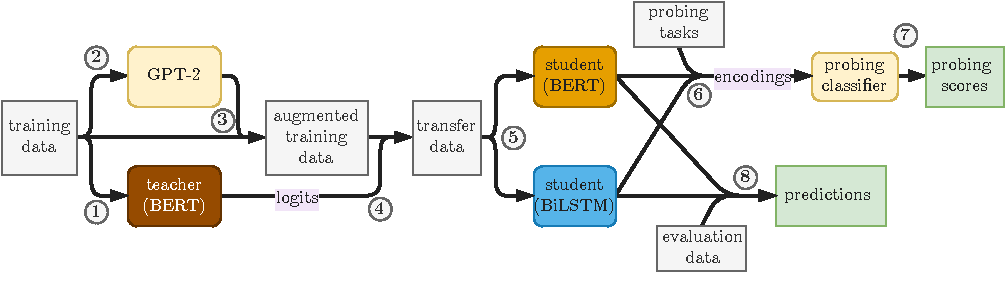
\includegraphics[width=17cm]{graphics/pipeline}}
      \cprotect\caption{The main pipeline of this work: \circled{1} teacher fine-tuning, \circled{2} GPT-2 fine-tuning, \circled{3} generating augmentation sentences, \circled{4} adding teacher logits to the augmented training dataset, \circled{5} knowledge distillation into students, \circled{6} producing probing sentence encodings, \circled{7} training the probing classifier and producing probing scores, \circled{8} producing predictions on evaluation sentences.}
      \label{fig:pipeline}
    \end{figure}

    For most of the implementation, the \verb|transformers| open-source PyTorch library \citep{Wolf_2019}\footnote{\rurl{github.com/huggingface/transformers}, accessed April 4, 2020}, is used, which provides tools for working with pre-trained Transformers like BERT. For knowledge distillation, I adapt the code of \citet{Sanh_2019}, which is today also part of \verb|transformers|\footnote{\rurl{github.com/huggingface/transformers/tree/master/examples/distillation}, accessed April 4, 2020}. (Note that the authors apply knowledge distillation \textit{before} downstream fine-tuning.) For augmenting the training data using GPT-2 and for knowledge distillation with the BiLSTM student, I adapt the code of \citeauthor{Tang_2019b}\footnote{\rurl{github.com/castorini/d-bert}, accessed April 4, 2020}, which uses an early version of \verb|transformers|. For probing the two students, the SentEval framework \citep{SentEval-paper}\footnote{\rurl{github.com/facebookresearch/SentEval}} is used.

    My own contributions to the implementation lie primarily in adapting and integrating the different codebases into one, and in adding the possibility for optimising a range of student hyperparameters. I also make the code more flexible, relative to the original codebases which encode numerous fixed design decisions made by \citeauthor{Sanh_2019} and \citeauthor{Tang_2019b}. The core of my implementation is open-sourced as a fork of the \verb|transformers| library at \rurl{github.com/samsucik/pytorch-transformers/}, while the implementation needed for individual experiemnts, analyses, and reporting, resides at \rurl{github.com/samsucik/knowledge-distil-bert}.
  }

  \section{Implementation details}{
    \label{sec:implementation-details}
    % teacher fine-tuning
    \subsection{Teacher fine-tuning}{
      Following \citet{Tang_2019b}, the case-insensitive pre-trained BERT\textsubscript{Large} is used as the teacher model (from now, referred to as \BERTT).
      With $L=24$ encoder layers, $A=16$ self-attention heads, the hidden dimension $d_h=1024$ and the indermediate dimension $d_I=4096$, the model has 340 million trainable parameters (as discussed in more detail previously in \autoref{sec:BERT}).
      The large BERT variant generally performs better than the 110-million-parameter BERT\textsubscript{Base} variant (both variants published by \citet{Devlin_2018}) and is therefore more attractive, but also slower, with a greater incentive for compression.

      \begin{table}[h!t]
      \centering
      \begin{tabular}{m{0.22\textwidth}|m{0.47\textwidth}}
      \hline
      loss function & cross-entropy \\
      \hline
      learning algorithm & Adam ($\eta=5\times10^{-5}$, $\beta_1=0.9$, $\beta_2=0.999$) \\
      \hline
      training budget & 3 epochs \\
      \hline
      $\eta$ scheduling & linear warm-up (first 10\% of training), then linear decay \\
      \hline
      batch size & 36 \\
      \hline
      dropout rate & 0.1 \\
      \hline
      \end{tabular}
      \caption{The fine-tuning configuration of the teacher BERT model.}
      \label{tab:initial-config-teacher}
      \end{table}

      For teacher fine-tuning on each downstream task, the procedure of \citeauthor{Tang_2019b} is used, summarised in \autoref{tab:initial-config-teacher}.
      While the performance of \BERTT~converges (flattens) within the 3-epoch training budget on CoLA and SST-2, the convergence is much slower for Sara. Hence, I empirically found a more suitable number of epochs within which the teacher converges on Sara: 10. See \autoref{fig:teacher-fine-tuning} for the evaluation-set performance of the teacher models and how they converge during fine-tuning.
      \begin{figure}[h!t]
        \centering
        \makebox[\textwidth][c]{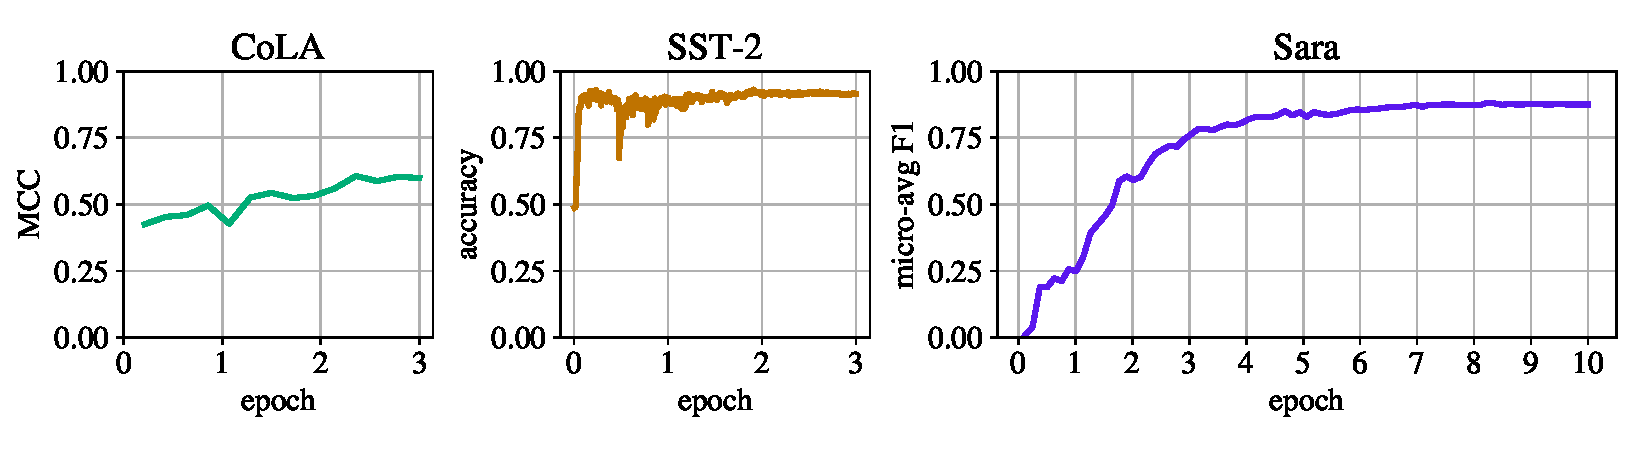
\includegraphics[width=15.5cm]{../experiments/analysis/img/teacher-fine-tuning}}
        \caption{The evaluation-set performance of teacher models across fine-tuning. Unintentionally, I used different logging frequencies in fine-tuning the teachers, hence the SST-2 plot is dense (and appears more noisy) while the CoLA plot is sparse.}
        \label{fig:teacher-fine-tuning}
      \end{figure}
    }

    % GPT-2 augmentation
    \subsection{Augmentation with GPT-2}{
      In fine-tuning the GPT-2 model, again the procedure of \citeauthor{Tang_2019b} is used (summarised in \autoref{tab:config-gpt-2}). This is very similar to the fine-tuning configuration used for \BERTT, with small differences. The AdamW learning algorithm is used \citep{Loshchilov_2019}, which is a variant of Adam with weight decay imposed on all learnable parameters, making the values slowly decay towards 0 in the absence of learning. The decay rate $\lambda$ determines the fraction by which each weight decays at each training step.
      The only parameter I choose differently from \citeauthor{Tang_2019b} is the batch size $B$: While they use batches of 48 examples, I only process examples in batches of 16, in order to make the fine-tuning possible with the limited memory resources.

      \begin{table}[h!t]
      \centering
      \begin{tabular}{m{0.22\textwidth}|m{0.48\textwidth}}
      \hline
      loss function & cross-entropy \\
      \hline
      learning algorithm & AdamW ($\eta=5\times10^{-5}$, $\beta_1=0.9$, $\beta_2=0.999$, $\lambda=1\times10^{-3}$) \\
      \hline
      training budget & 1 epoch \\
      \hline
      $\eta$ scheduling & linear warm-up (first 10\% of training), then linear decay \\
      \hline
      batch size & 16 \\
      \hline
      dropout rate & 0.1 \\
      \hline
      \end{tabular}
      \caption{The fine-tuning configuration of the GPT-2 model.}
      \label{tab:config-gpt-2}
      \end{table}
    }

    % student architectures + default params
    \subsection{BiLSTM student model}{
      \label{sec:student-bilstm}
      As the first student, I use the bi-directional LSTM (BiLSTM) from \citeauthor{Tang_2019b} (see \autoref{fig:bilstm}). The model comprises in particular one hidden BiLSTM layer with 300 units, which is composed of two LSTM layers processing the inputs in opposite directions. The last hidden states for either of the two processing directions are concatenated and passed to a fully connected layer with 400 output units\footnote{Even though \citeauthor{Tang_2019b} tried also other, slightly different layer dimensions, these are the ones that worked the best on CoLA.}, which uses the rectified linear unit (ReLU) activation function \citep{Nair_2010}, and dropout. A final (linear) layer follows, projecting to the number of target classes, i.e. producing the logits. The model is topped with a softmax classifier for normalising the logits and producing class probabilities.
      \begin{figure}[h!t]
        \centering
        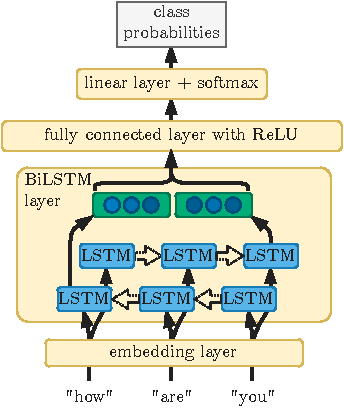
\includegraphics[width=7cm]{graphics/bilstm}
        \caption{The bi-directional LSTM student. Diagram adapted from Figure 1 of \citet{Tang_2019a}.}
        \label{fig:bilstm}
      \end{figure}

      The original model was built to process sentences word by word, encoding each word using the pre-trained word2vec embeddings\footnote{The 300-dimensional version trained on Google News, see \rurl{code.google.com/archive/p/word2vec/}.} before passing it to the LSTM layer. Words for which there is no embedding (\textit{out-of-vocabulary} words, or just OOV) are embedded using a vector initialised with random numbers drawn uniformly from [-0.25, 0.25]. The embedding layer supports three \textit{embedding modes}, based on \citet{Kim_2014}:
      \begin{enumerate}
        \item \textbf{Static}: the embedding parameters are frozen and do not change during training.
        \item \textbf{Non-static}: the embedding parameters are allowed to change (fine-tune) during training.
        \item \textbf{Multichannel}: two embedding instances are used in parallel, one is frozen, the other one is allowed to change. For each input word, the two embeddings produced are concatenated together for further processing. The multichannel mode is the one used by \citeauthor{Tang_2019b}.
      \end{enumerate}

      One significant change I made to this model is enabling the use of wordpiece embeddings instead of word-level ones. This way, the fine-tuned embedding parameters from \BERTT~can be used to initialised the student's embedding layer, providing some of the teacher's ``knowledge'' even before the student training (knowledge distillation) begins.

      When the word2vec embeddings are used, the embedding matrix of the LSTM is constructed in the following way:
      \begin{enumerate}
        \item A vocabulary of all distinct words present in the transfer dataset is made.
        \item Only the word2vec vectors corresponding to these words are taken and put together to create the embedding matrix.
      \end{enumerate}
      This way, even though the full word2vec collection covers 3,000,000 words, the word-level embedding matrix (whether used by the LSTM student or the BERT student) has fewer entries. For the particular transfer datasets I use, the vocabulary has 243,120 words for CoLA, 284,273 words for SST-2, and 172,183 words for Sara.

      In total, this model -- from now referred to as \LSTMS~-- has 2.41 million trainable parameters (excluding the embedding layer), making it 140x smaller than \BERTT.
    }

    \subsection{BERT student model}{
      For the second student, a down-scaled version of BERT\textsubscript{Large} is used, matched for size with \LSTMS. In particular, I scale all the dimensions of BERT\textsubscript{Large} down by a factor of \mytilde5, leading to a smaller BERT with $L=5$ encoder layers, the hidden dimension $d_h=204$, the intermediate dimension $d_I=750$, and $A=3$ self-attentional heads -- amounting to 2.42 million trainable parameters (embedding parameters excluded). This model is from now referred to as \BERTS.
    }

    % knowledge distillation + default params 
    % mention that KD is like normal training given the transfer set
    \subsection{Knowledge distillation}{
      While \autoref{tab:initial-configs} summarises the initial configuration of both student models, I elaborate more on these parameters in the rest of this section.

      During knowledge distillation, \BERTS~is trained using the cross-entropy loss. The softmax temperature is fixed at $T=3$.\footnote{Usual values are from 1 (no effect) to 3. For instance, \citet{Sanh_2019} use $T=2$. In a work that is much close to my situation, \citet{Tsai_2019} apply knowledge distillation from BERT\textsubscript{Base} into a 18-million-parameter smaller BERT, observing that from $T=\{1, 2, 3\}$ the best one was $T=3$.}
      
      Originally, both students were implemented to use random initialisation from scratch before training, with the exception of the embedding layer of \LSTMS, which was initalised from word2vec. Later, I explore different ways of initialising the embedding layers.
      
      During training, \LSTMS~uses the mean squared error (MSE) loss, following \citeauthor{Tang_2019b} who report that MSE led to slightly better performance (compared to cross-entropy loss with $T=3$). Following preliminary experiments on CoLA, I set the training budget to 30 epochs for \LSTMS~(same as \citeauthor{Tang_2019b}). \BERTS~converges slower and therefore uses a 60-epoch training budget in all following experiments. In student training, the evaluation-set performance reported is always for the best model checkpoint as observed during training; in particular, it may not be the final model version.
      Using this approach, even if a student's performance eventually starts to decrease during training, the best-performing version is retained for further analysis and comparison.

      % The learning algorithm is Adam for \BERTS, with $\beta_1=0.9$ and $\beta_2=0.98$ (the defaults in \verb|transformers|). The learning rate was initially set to $5\times10^{-4}$ and later optimise.
      Following \citeauthor{Tang_2019b}, the Adadelta learning algorithm \citep{Zeiler_2012} is used for training \LSTMS, with $\eta=1.0$ and $\rho=0.95$, while Adam is used for \BERTS.
      Note that Adam is an improved successor of Adadelta\footnote{In particular, the adaptive mechanism of Adadelta considers only the recent squared gradient magnitudes, whereas Adam also considers the simple (not squared) gradients.} and is much more widely used; later in this work, I explore the use of Adam for \LSTMS. No $\eta$ scheduling is used with \LSTMS, while \BERTT~uses scheduling similar to \BERTT.
      % For \BERTS, I originally anneal $\eta$ linearly from 0 over the first 10 epochs, and let it linearly decay to 0 during the remaining 50 epochs. Later, I explore other annealing schedules.
      To prevent ``gradient explosion'' in \LSTMS, the total magnitude of all gradients is clipped to 30.0 before every parameter update (as used by \citeauthor{Tang_2019b}); however, throughout all experiments, I never observe the gradient norm to reach this limit.
      For more robust training, the standard dropout rate of 0.1 is used during training of both students, following \citet{Devlin_2018} and \citeauthor{Tang_2019b}.
      \citeauthor{Tang_2019b} report the small batch size $B=50$ to work well with the BiLSTM student. For \BERTS, I initially use a larger batch size $B=256$.

      While LSTMs can process sequences of any lengths, Transformer models like BERT impose a maximum sequence length for practical reasons, with all sequences within a batch padded to the maximum length. Although \BERTT~allows sequences of up to 512 wordpieces in length, extremely few sentences reach this length -- especially in this work, where all inputs are single sentences, not sentence pairs. Therefore, to accelerate training, I use the maximum sentence length of 128 tokens for \BERTS.

      \begin{table}[h!tb]
      \centering
      \begin{tabular}{m{0.22\textwidth}|m{0.32\textwidth}|m{0.35\textwidth}}
      & \LSTMS & \BERTS \\
      \hline
      loss function & mean square error & cross-entropy, $T=3$ \\
      \hline
      learning algorithm & Adadelta ($\eta=1.0$, $\rho=0.95$) &  Adam ($\eta=5\times10^{-4}$, $\beta_1=0.9$, $\beta_2=0.98$) \\
      \hline
      training budget & 30 epochs & 60 epochs \\
      \hline
      $\eta$ scheduling &  & linear warm-up (10 epochs), then linear decay \\
      \hline
      batch size & 50 & 256 \\
      \hline
      embedding layer initialisation & word2vec & wordpiece, from \BERTT \\
      \hline
      \end{tabular}
      \caption{The initial parameters of both student models.}
      \label{tab:initial-configs}
      \end{table}
    }

    % probing
    \subsection{Probing}{
      \label{sec:implementation-details-probing}
      For the light-weight probing classifier, \citet{Conneau_2018} use a small neural network comprising one hidden layer with the sigmoid activation function and dropout, followed by a linear layer projecting to the desired number of classes. 
      In training the classifier, early stopping is used, i.e. training stops when the evaluation-set accuracy does not improve over 5 consecutive iterations.
      For consistency with the exact method of \citeauthor{Conneau_2018}, I tune the dropout rate (choosing from [0.0, 0.1, 0.2]) and the hidden layer width (choosing from [50, 100, 200]) using the evaluation set. Each probing score is reported as the one for the best dropout and layer width values.
      \autoref{tab:config-probing-classifier} summmarises all important training parameters.

       % The cross-entropy loss is used, with the Adam learning algorithm with $\eta=0.001$, $\beta_1=0.9$ and $\beta_2=0.999$. 
      \begin{table}[h!t]
      \centering
      \begin{tabular}{m{0.21\textwidth}|m{0.47\textwidth}}
      \hline
      loss function & cross-entropy \\
      \hline
      learning algorithm & Adam ($\eta=1\times10^{-3}$, $\beta_1=0.9$, $\beta_2=0.999$) \\
      \hline
      training budget & 4 epochs (early stopping) \\
      \hline
      batch size & 64 \\
      \hline
      dropout rate &  [0.0, 0.1, 0.2]\\
      \hline
      \end{tabular}
      \caption{The training configuration of the probing classifier.}
      \label{tab:config-probing-classifier}
      \end{table}

      When probing a model, an important design decision is how to extract sentence representations from the model's layers.
      The BiLSTM layer of \LSTMS~can produce at each timestep two hidden states (one for each processing direction). \citeauthor{Conneau_2018} experiment with:
      \begin{enumerate}
        \item Creating a \textit{BiLSTM-max} encoding such that each of its elements is the maximum over the values for each timestep. (The encoding has the same dimensionality as the BiLSTM layer output.)
        \item Creating a \textit{BiLSTM-last} encoding by simply taking the last hidden state in each direction -- the encoding is the same as the BiLSTM layer output.
      \end{enumerate}
      \citeauthor{Conneau_2018} report mixed results, with BiLSTM-max encodings leading to better probing scores on some of the probing tasks. I am constrained to using BiLSTM-last since the PyTorch implementation of LSTMs does not give access to intermediate hidden states, only to the last one in each direction.

      In BERT, all hidden representations produced by each encoder layer can be accessed. I try three different ways of combining a sequence of hidden representations from a particular layer into a single encoding:
      \begin{enumerate}
        \item Maximum pooling, equivalent to BiLSTM-max: Taking the maximum value for each element over all hidden representations.
        \item Single-position encoding (the equivalent of BiLSTM-last): Taking the hidden representation that is used for the final classification. While in \LSTMS, this would mean taking the last hidden state in each direction, in BERT, it is the hidden representation of the first token (the special \verb|[CLS]|).
        \item Average pooling (not explored by \citeauthor{Conneau_2018}): Similarly to maximum pooling, this uses the average of each element across all representations.
      \end{enumerate}
      After conducting simple preliminary probing experiments with \BERTT~on each downstream task, I observed that the differences between the three approaches are mostly inconsistent and small. However, in many cases, maximum pooling produced worse probing scores than the other two techniques, and average pooling slightly outperformed single-position representations. In all further probing experiments with \BERTT~and \BERTS, the average pooling approach is used.

      Inspired by the localisation experiments of \citet{Tenney_2019b}, I probe various encoder layers across the BERT models in order to also localise each type of language knowledge within the model's architecture.
    }
  }

  \section{Computing environment and runtimes}{
    All major parts of my experiments -- teacher and GPT-2 fine-tuning, augmentation data sampling, teacher logits generation, knowledge distillation and probing -- are run in the environment of the University's Teaching cluster\footnote{\rurl{computing.help.inf.ed.ac.uk/teaching-cluster}.}.

    Each job uses its own one Nvidia GPU -- either GeForce GTX TITAN X or GeForce RTX 2080 Ti -- with 12-13GB of memory, and additional 30GB of RAM for use with CPU processes.

    \begin{table}[h!t]
    \centering
    \begin{tabular}{m{0.32\textwidth}|c|c|c}
    % \hline
    & CoLA & SST-2 & Sara \\
    \hline
    teacher fine-tuning & $\sim$30min & $\sim$4h & $\sim$55min \\
    \hline
    GPT-2 fine-tuning & 3min & 31min & 1min \\
    \hline
    augmentation data sampling & 17h & 15h & 4h \\
    \hline
    teacher logits generation & $\sim$1h & $\sim$8h & $\sim$2h \\
    \hline
    \LSTMS~training & $\sim$5h & $\sim$8h & $\sim$6h \\
    \hline
    \BERTS~training & $\sim$15h & $\sim$26h & $\sim$22h \\
    \hline
    \end{tabular}
    \caption{The runtimes for all steps of knowledge distillation with augmented transfer datasets.}
    \label{tab:runtimes}
    \end{table}

    All important runtimes are reported in \autoref{tab:runtimes}\footnote{Note that the only processes that are parallelised are the augmentation data sampling and the teacher logits generation -- both use 4 parallel threads, each with its own GPU with 6GB of memory. In logits generation, examples are processed in batches of 2048 in each thread.}.
    The reason why all steps take the longest on SST-2 is 1) the amount of training data (almost 10x more than for CoLA), and 2) the fact that sentences in SST-2 are longer than those in CoLA and Sara.
    Interestingly, even though \LSTMS~and \BERTS~are of similar size, the BERT model takes much longer to train -- likely because it is much deeper.

    Because of the role restrictions in the cluster, I cannot run more than 20 jobs at the same time. This has a significant impact especially on the time it takes to run the hyperparameter exploration experiments (see the next chapter). 
    It is also the main reason why I do not -- with a few exceptions -- repeat experiments with varying random seeds for more robust results. 

    % CoLA: end of epoch 1 | loss 0.86 | ppl  89.79 | bpc 1.237 | 02:56
    % SST-2:end of epoch 1 | loss 0.90 | ppl  75.52 | bpc 1.296 | 31:02
    % Sara: end of epoch 1 | loss 0.94 | ppl 111.48 | bpc 1.363 | 00:55
  }

  \section{Conclusions \reviewready}{
    % aims: insights, nt numbers
    In this chapter, I presented the high-level set up as well as the implementation details of all experiments.
    % implementation: work of others
    Importantly, the main outcomes of this exploratory work are intended to be insights, not improved performance scores.
    % my own work: combining; introducing small bert; and analysis (probing across layers; new probing encoding extraction technique!)
    With most of the programming efforts going into adapting and integrating existing codebases, my original contributions are mostly intellectual: 
    Using two architecturally different students side by side; 
    using the probing suite of \citet{Conneau_2018} for localisation of linguistic knowledge;
    using a new technique for extracting probing encodings; 
    and later manually analysing the predictions made by the teacher and student models.
    % KD very slow, need to think twice before experiments
  }
}

\chapter{Training student models \reviewready}{
  % - aims: small, good, 90\% of teacher's score
  In this chapter, I use knowledge distillation to train student models \BERTS~and \LSTMS~from the fine-tuned teacher \BERTT~on each of the three downstream tasks.
  My aim is to end up with students that are small but perform well. Ideally, the student size will stay at the initial 2.4 millions of trainable non-embedding parameters while the evaluation-set performance will be above 90\% of the teacher's performance.

  As discussed in \autoref{sec:methods}, my aim is not to find the best possible student hyperparameters, but I still explore some of them to gain an intuition for the reasonable ranges of values and for their behaviour in knowledge distillation.
  In particular, I find a well-performing configuration of each student on CoLA, looking for good evaluation-set score and fast convergence. Then, on the remaining tasks, I use the same configuration, only tailoring a small number of parameters to the need of the concrete dataset at hand. Most importantly, I adjust the size of each student separately for each task because some tasks are known to be more or less difficult than others, requiring the students to be more or less complex.

  After obtaining well-performing students for each task, I compare them with one another and with the respective teacher and discuss my observations.

  \section{General hyperparameter exploration on CoLA}{
    \label{sec:hparam-general}

    I restrict myself to exploring the following essential hyperparameters (in both students):
    \begin{enumerate}
      \item $\eta$ -- the learning rate. Additionally, for \LSTMS, I compare the original Adadelta learning algorithm with the more general Adam.
      \item Learning rate scheduling, more concretely the warmup duration (in epochs) $E_{w}$ of gradual warmup of the learning rate \citep{Goyal_2017}, and the optional use of linear decay following the warmup.
      \item $B$ -- the minibatch size.
      \item Embedding type -- word-level vs wordpiece.
    \end{enumerate}

      % \item Embedding mode -- one of static, non-static, and multi-channel (discussed in \autoref{sec:student-bilstm}).
    Following on the discussion of implementation details in \autoref{sec:implementation-details}, the initial configurations of the parameters to be explored are:
    \begin{itemize}
      \item For \BERTS: Adam with $\eta=5\times10^{-5}$, $B=256$, $E_{w}=10$ -- warmup over the first 10 epochs, followed by linear decay of $\eta$, and wordpiece embedding layer with the non-static mode.
      \item For \LSTMS: Adadelta with $\eta=1.0$, $B=50$, no $\eta$ warmup or decay, and the word-level embeddings with the multichannel mode.
    \end{itemize}
    Note that the embedding mode is explored separately for each task in the next section.

    Initially, \BERTS~was initialised entirely from scratch, including the embedding layer. 
    This may pose a disadvantage for \BERTS~because the BiLSTM student starts with embeddings initialised from the pre-trained word2vec. To eliminate this disparity, I initialise \BERTS's wordpiece embeddings using the parameters from the fine-tuned \BERTT. 
    Because the teacher's embeddings are high-dimensional (1024-D), a trainable linear layer is used inside \BERTS~to project them to $d_h=204$ dimensions\footnote{The token type and positional embeddings are not initialised from the teacher and hence do not require dimensionality reduction. They are added to the wordpiece embeddings after these are dimensionality-reduced.}.
    Even though the idea of initialising one model with another one's parameters is not new, to the best of my knowledge, I am the first one to initialise a student in knowledge distillation from Transformers in this way.
    In exploring the parameters of \BERTS, I report results for the variant with the teacher's embedding knowledge. Results for the variant initialised entirely from scratch are in \textbf{TO-DO: APPENDIX X}.
    In general, the difference is not large, but the version initialised from scratch performs slightly worse.
    
    \subsection{Choosing learning algorithm and learning rate}{
      Because \citet{Tang_2019b} report not tuning their BiLSTM hyperparameters, I verify their choices.
      In particular, the use of the Adam learning algorithm is explored -- a widely used and improved version of the Adadelta algorithm which is used originally.

      For both students, I try a wide range of $\eta$ values with Adam: $5\times10^{-3},\ 1.5\times10^{-3},\ 5\times10^{-4},\ 1.5\times10^{-4},\ 5\times10^{-5},\ 1.5\times10^{-5},\ 5\times10^{-6}$.
      
      \begin{figure}[h!t]
        \centering
        \makebox[\textwidth][c]{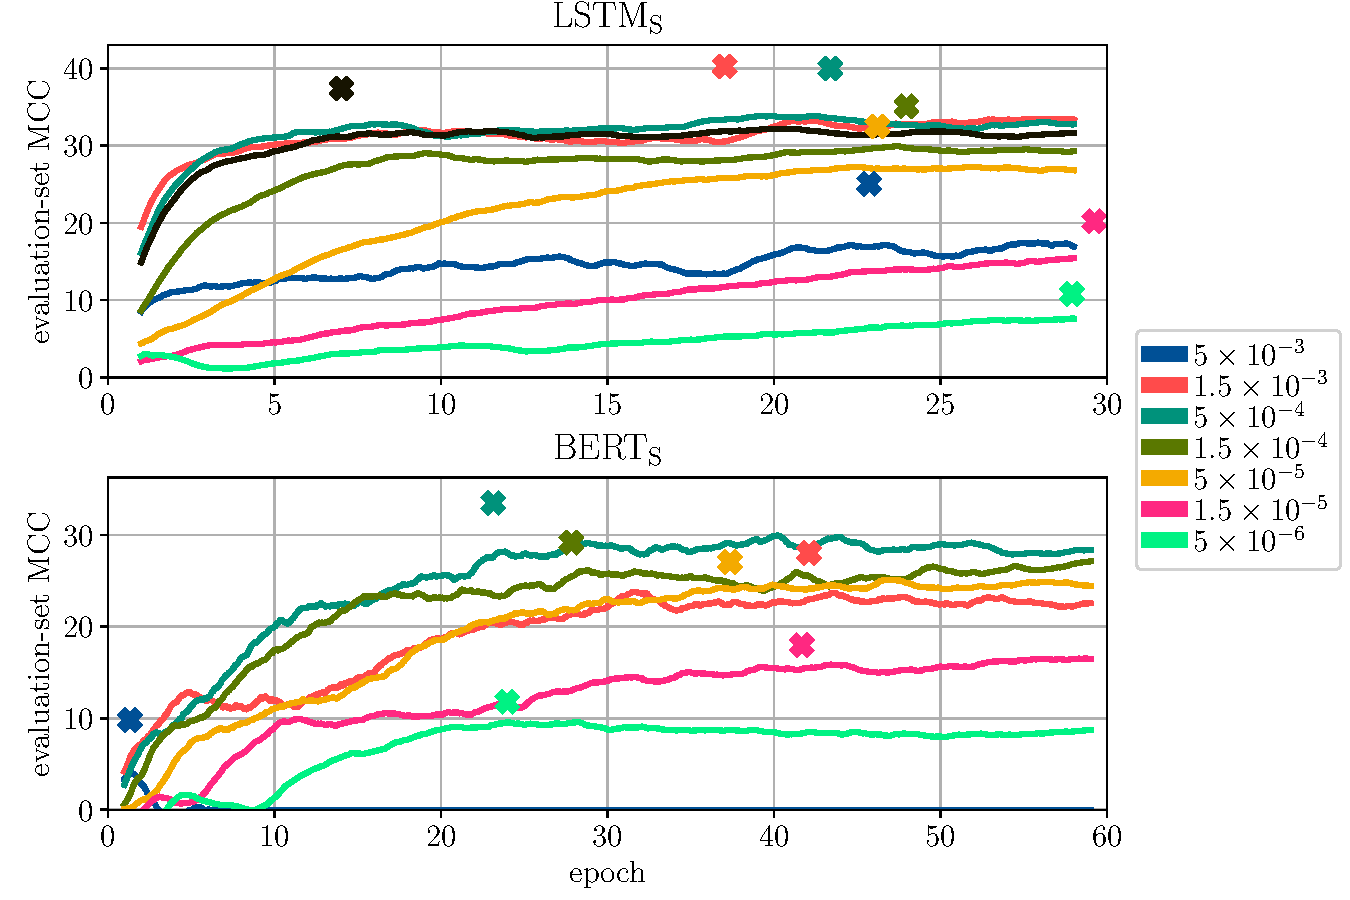
\includegraphics[width=14.8cm]{../experiments/analysis/img/exploration-lr}}
        \caption{Comparing various $\eta$ values on CoLA. Crosses mark the maximum scores. \sliding}
        \label{fig:exploration-lr}
      \end{figure}

      \autoref{fig:exploration-lr} shows that for all students the ideal $\eta$ is around $5\times10^{-4}$. Much larger and much smaller values leading to poor learning, in particular the largest $\eta=5\times10^{-3}$ ``kills'' the learning of \BERTS~entirely due to gradient explosion.
      As expected, \BERTS~initialised from scratch performs worse than when initialised from the wordpiece embeddings of \BERTT. However, the differences are not large.

      As discussed previously, \BERTS~converges much slower than \LSTMS, hence the 30-epoch and 60-epoch training budgets for \LSTMS~and \BERTS, respectively. Additionally, it is apparent that \LSTMS~performs significantly better than \BERTS~even though the sizes of the models are comparable.

      In the case of \LSTMS, the Adadelta algorithm is outperformed by Adam. From now onwards, I use Adam with both students, in all cases with $\eta=5\times10^{-4}$.
    }

    \subsection{Choosing learning rate scheduling and batch size}{
      \citet{Tang_2019a} use no learning rate scheduling, but they report small batch sizes ($B=50$) to work better than the usual, larger batches. Hence, for \LSTMS~I first verify their claims and subsequently move on to $\eta$ scheduling. For \BERTS, inspired by \citet{Sanh_2019} who take advantage of scheduling (both in terms of warmup and decay), I explore $\eta$ scheduling first (as a continuation from exploring $\eta$ values), and then look at various $B$ values.

      \begin{figure}[h!t]
        \centering
        \makebox[\textwidth][c]{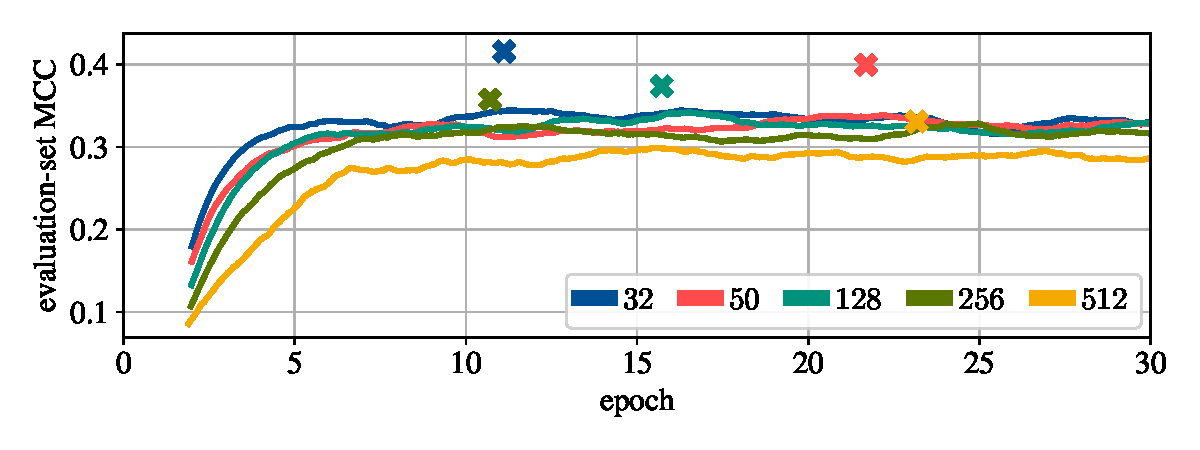
\includegraphics[width=14cm]{../experiments/analysis/img/exploration-B-lstm}}
        \caption{Comparing various batch sizes for \LSTMS~on CoLA. Crosses mark the maximum scores. \sliding}
        \label{fig:exploration-B-lstm}
      \end{figure}

      As \autoref{fig:exploration-B-lstm} shows, \LSTMS~clearly does prefer small batch sizes. However, training with tiny minibatches takes very long -- compare \mytilde25min for $B=512$ with \mytilde7h for $B=32$. Hence, I restrain from trying even smaller batch sizes and use $B=32$ for \LSTMS~in all further experiments.

      \begin{figure}[h!t]
        \centering
        \makebox[\textwidth][c]{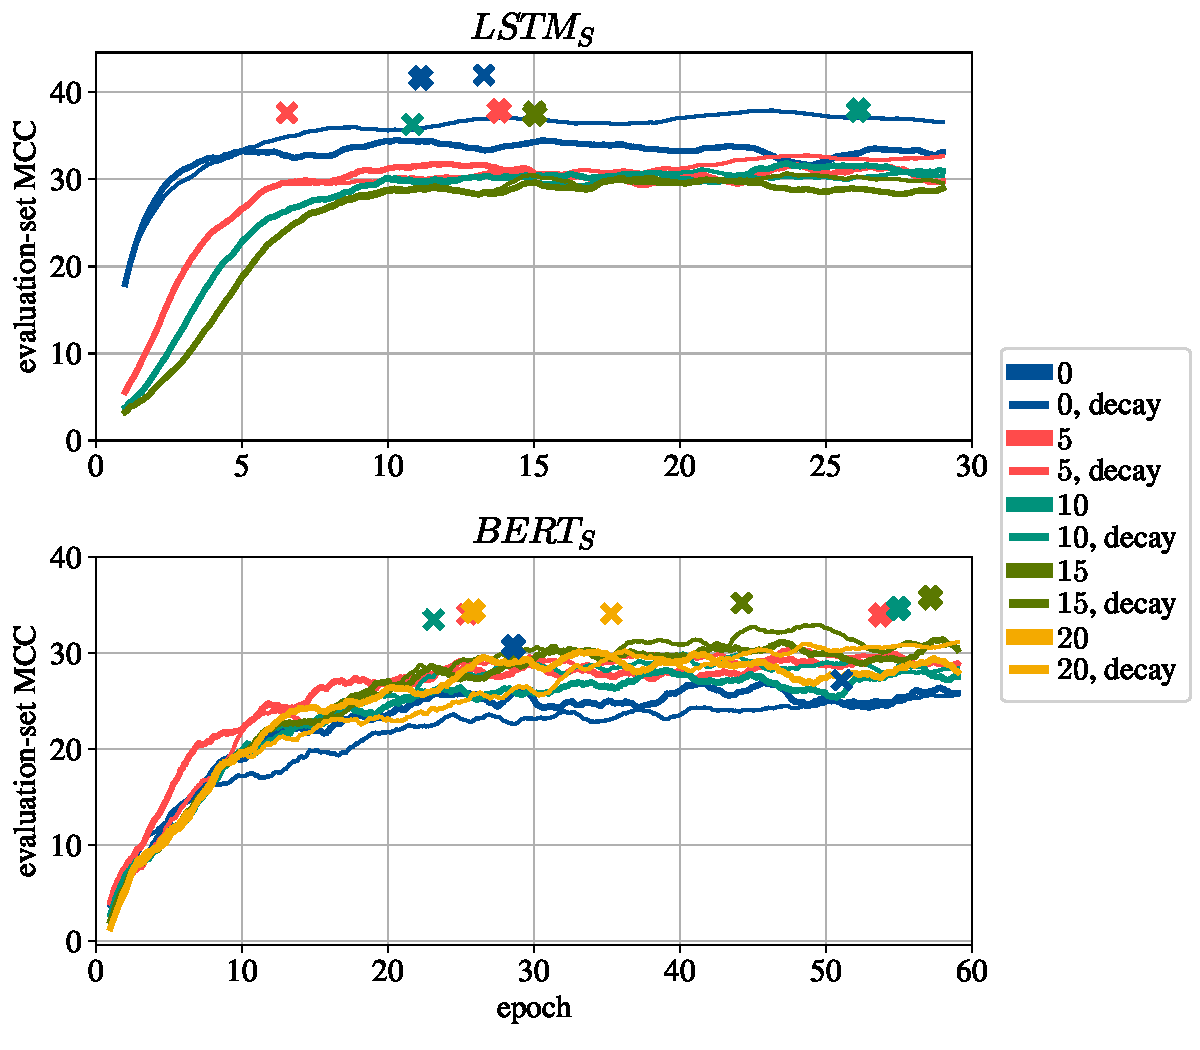
\includegraphics[width=13.5cm]{../experiments/analysis/img/exploration-schedule}}
        \caption{Comparing warmup durations $E_w$ on CoLA, with the optional learning rate decay to 0 over the remaining training epochs. Crosses mark the maximum scores. \sliding}
        \label{fig:exploration-schedule}
      \end{figure}

      \autoref{fig:exploration-schedule} shows the results of exploring various warmup durations for both students. Note that for \LSTMS, whose training budget is only 30 epochs, I did not try the long warmup duration of 20 epochs, only up to 15 epochs.

      In the case of \LSTMS, \autoref{fig:exploration-schedule} shows that the longer the warmup duration, the slower the model converges. This is understandable because during warmup, learning happens less aggressively -- and hence more slowly -- due to the smaller learning rate. More importantly, the graph shows that $\eta$ decay does not significantly affect training, but it can help to prevent the model from overfitting the training data. This is most visible for $E_w=0$ where \LSTMS's performance starts to slowly decrease after 20 epochs in the absence of $\eta$ decay. All in all, using the full $\eta$ from the beginning of training is the best option, and $\eta$ decay can only improve things. $E_w=0$ with decay is used for \LSTMS~in all further experiments.

      In the case of \BERTS, the only clear result visible from \autoref{fig:exploration-schedule} is that \BERTS~performs poorly without $\eta$ warmup. For non-zero warmup durations, there are no significant differences in the best-performance points (marked by crosses) or in the convergence speed. In all further experiments with \BERTS, I use $E_w=15$ and $\eta$ decay -- the configuration which shows the highest stable performance level in \autoref{fig:exploration-schedule} in later epochs (beyond epoch 35).

      \begin{figure}[h!t]
        \centering
        \makebox[\textwidth][c]{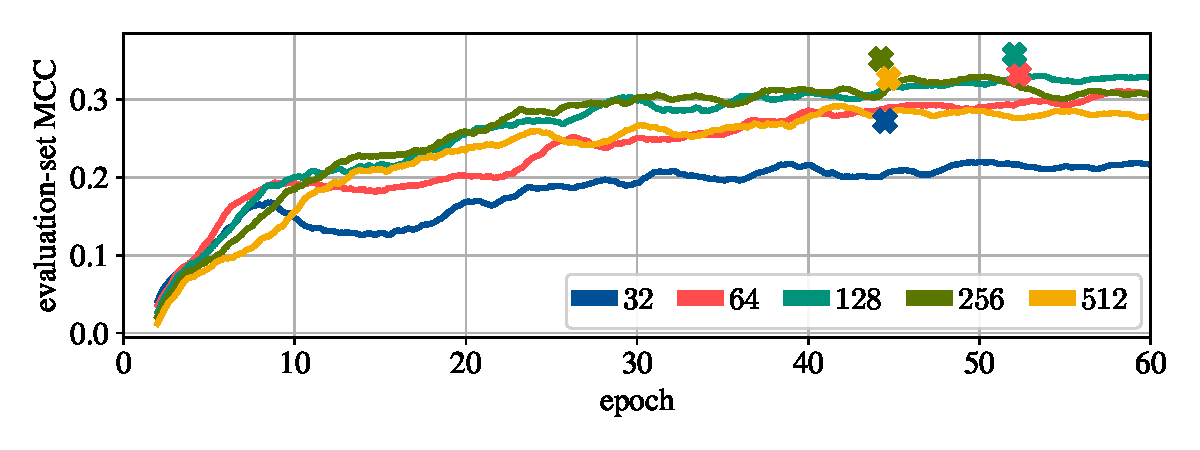
\includegraphics[width=14cm]{../experiments/analysis/img/exploration-B-bert}}
        \caption{Comparing various batch sizes for \BERTS~on CoLA. Crosses mark the maximum scores. \sliding}
        \label{fig:exploration-B-bert}
      \end{figure}

      The batch size exploration in \autoref{fig:exploration-B-bert} shows that \BERTS~performs best with mid-sized batches of 128-256 examples. Too large batch size ($B=512$) as well as very small batches of 32-64 make \BERTS~underperform (with tiny batches of 32 being particularly detrimental).
      In all further experiments, $B=128$ is used with \BERTS.
    }
  }

  \section{Optimising students for each downstream task}{
    In this section, I explore different ways of initialising student models with language knowledge, and the effect of model size, separately for each downstream task.

    \subsection{Choosing embedding type and mode}{
      In the previous section, \LSTMS~consistently outperformed \BERTS. This can be due to different model architectures or due to different embedding types and modes -- while \LSTMS~has its word-level embedding layer initialised using word2vec and uses the multichannel mode\footnote{I.e. uses two parallel embedding table instances, one frozen and the other one allowed to further change in training.}, \BERTS~uses wordpiece-level embeddings from the fine-tuned \BERTT~in the non-static mode\footnote{This is the usual case where a single embedding table instance is used and allowed to change during training.}.

      I explore combinations of the two embedding types and of different embedding modes. Following preliminary experiments, I do not use the static (embedding freezing) mode as it has detrimental effects on student learning. Left for exploration are the two modes that do allow embedding parameters to be tuned during training: the multichannel and non-static modes.

      \begin{figure}[h!t]
        \centering
        \makebox[\textwidth][c]{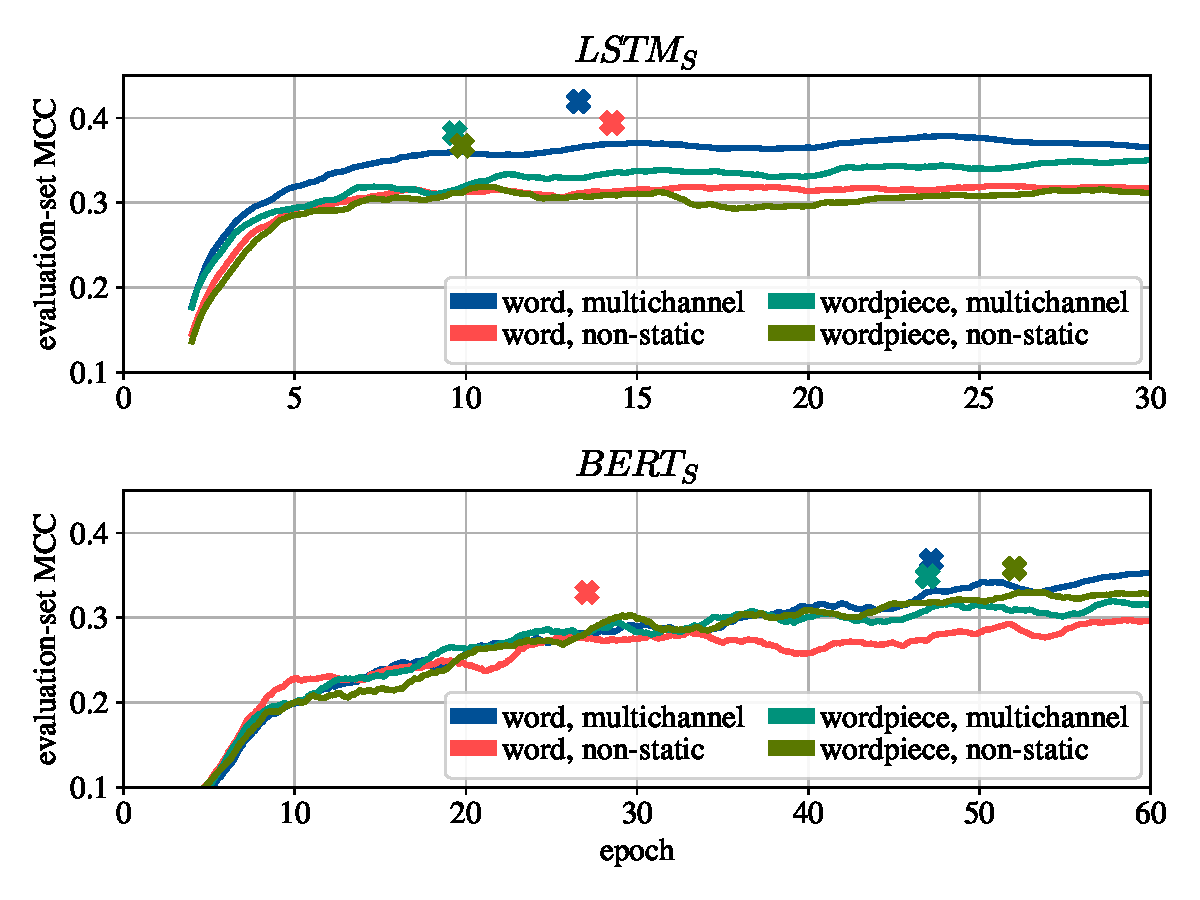
\includegraphics[width=14cm]{../experiments/analysis/img/exploration-embed-cola}}
        \caption{Comparing embedding types and modes on CoLA. Crosses mark the maximum scores. \sliding}
        \label{fig:exploration-embed-cola}
      \end{figure}

      \autoref{fig:exploration-embed-cola} shows how different type and mode combinations affect knowledge distillation on CoLA. With \LSTMS, the multichannel mode is preferred to non-static and word2vec embeddings are preferred to wordpieces; hence, I use the multichannel mode with word2vec in further experiments (same as \citet{Tang_2019b}). For \BERTS, the differences are smaller, yet it is clear that word-level embeddings benefit from using the frozen and unfrozen versions provided by the multichannel mode. In further experiments, the multichannel mode combined with word-level word2vec embeddings is used.

      For SST-2, I only compare the best word-level and the best wordpiece-level combination for each model as observed from \autoref{fig:exploration-embed-cola}. The results are shown in \autoref{fig:exploration-embed-sst-2}. Notice the scale of the y axis: In particular, the students perform roughly the same (unlike on CoLA) and any relative differences observed in \autoref{fig:exploration-embed-sst-2} are much smaller than the differences observed on CoLA in \autoref{fig:exploration-embed-cola}. Hence, I refrain from making conclusions about which embedding type and mode works better; I merely choose to use the word-level embeddings with the multichannel mode in all further experiments on SST-2 (my decision is based on the best evaluation scores marked by crosses in \autoref{fig:exploration-embed-sst-2}).

      \begin{figure}[h!t]
        \centering
        \makebox[\textwidth][c]{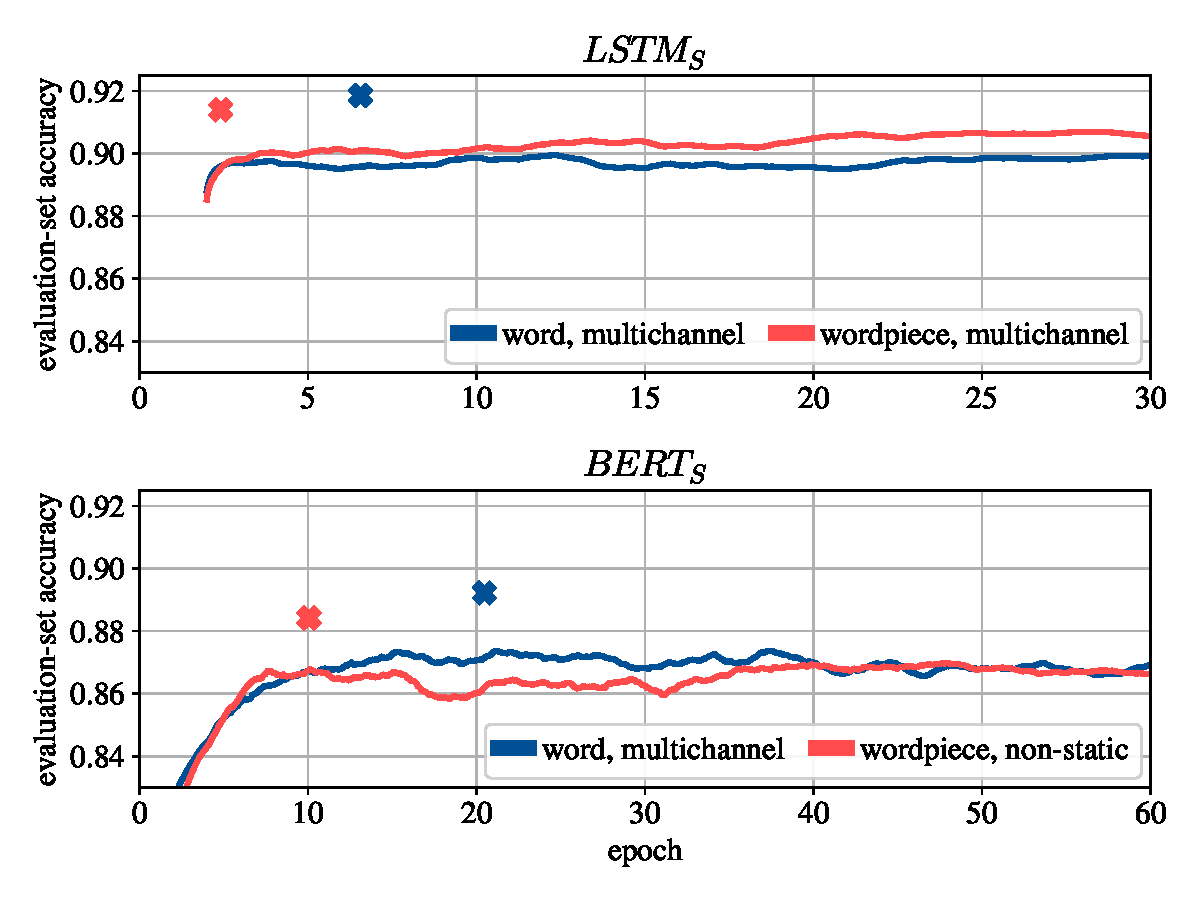
\includegraphics[width=14cm]{../experiments/analysis/img/exploration-embed-sst-2}}
        \caption{Comparing embedding types and modes on SST-2. Crosses mark the maximum scores. \sliding}
        \label{fig:exploration-embed-sst-2}
      \end{figure}

      Results on Sara are shown in \autoref{fig:exploration-embed-sara}. Here again, the relative differences in performance are small, but using wordpieces helps both students converge faster and reach slightly better performance levels. This can be a result of the word2vec vocabulary not capturing well the conversational language in Sara examples, for instance the utterance ``yesyesyes'' would be treated simply as one out-of-vocabulary word, whereas wordpieces have the potential to encode it as the word ``yes'' repeated 3x. In all further experiments on Sara I use the wordpiece embeddings, using the multichannel mode in \LSTMS~and the non-static mode in \BERTS.

      \begin{figure}[h!t]
        \centering
        \makebox[\textwidth][c]{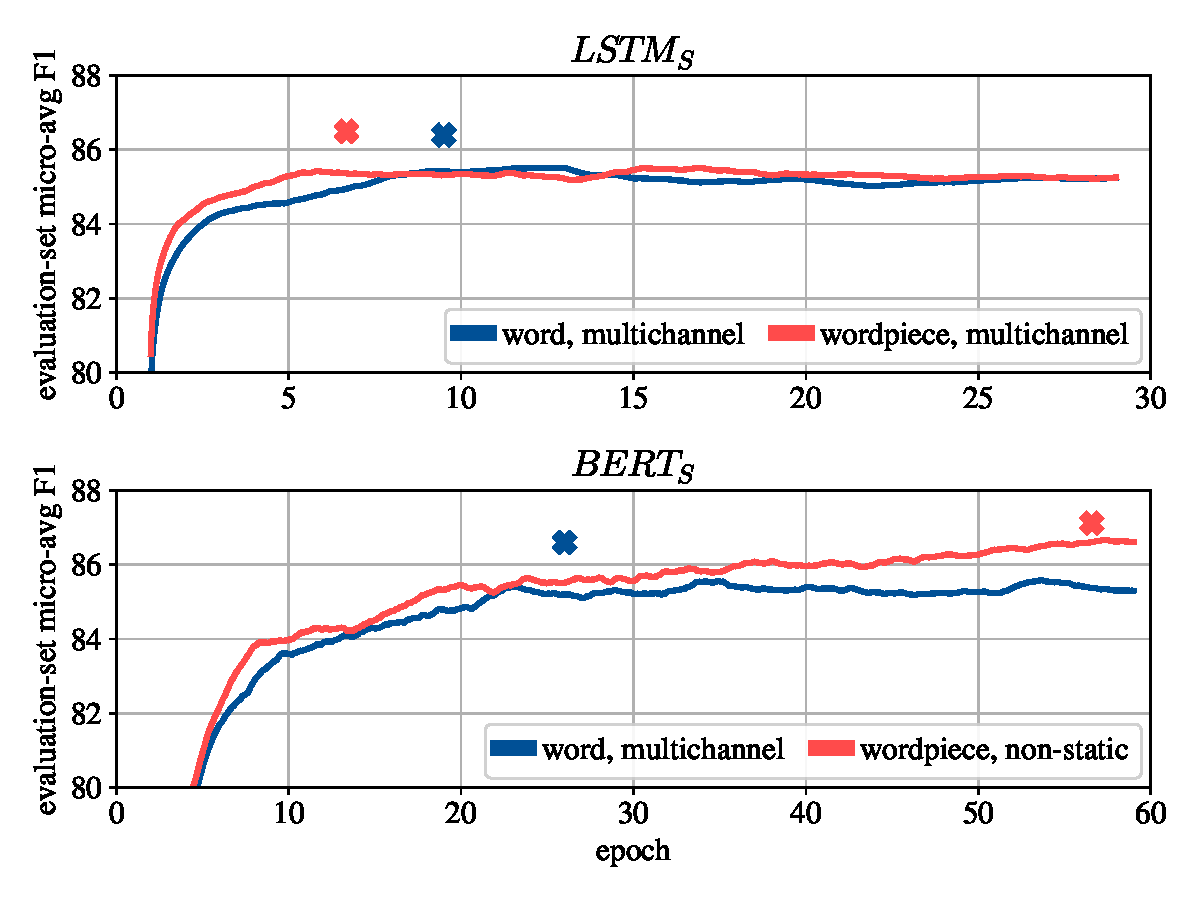
\includegraphics[width=14cm]{../experiments/analysis/img/exploration-embed-sara}}
        \caption{Comparing embedding types and modes on Sara. Crosses mark the maximum scores. \sliding}
        \label{fig:exploration-embed-sara}
      \end{figure}

      All in all, the multichannel mode seems to be generally superior to the non-static mode which lacks the frozen version of embeddings. Initialisation from the word-level word2vec embeddings also works better than wordpieces where examples tend to contain legitimate English (CoLA and SST-2). As for the performance gap between \LSTMS~and \BERTS, I conclude that it cannot be explained by differences in embedding type/mode, and is most likely a consequence of different student architectures.

      While wordpiece embeddings have the advantage of being fine-tuned on the particular downstream task (as part of teacher fine-tuning), word2vec contains more general knowledge stored at the word level.
      Importantly, the wordpiece vocabulary contains the most frequent words in their entirety; only the less frequent ones are split into pieces.
      Thus, for frequent words, their word2vec and wordpiece embeddings will differ only in the way they are trained.
      Naturally, since the wordpiece vocabulary has only 30,522 tokens while word2vec has 3,000,000, there are many words covered by word2vec for which the wordpiece embeddings have to be assembled from multiple pieces. On these words -- frequent enough to be in the word2vec vocabulary, but not the most frequent ones -- word2vec could have an advantage.
      Once we move beyond the words covered by word2vec to rare tokens like ``yesyesyes'', wordpieces become the preferred approach.
      Clearly, no one approach is generally the best, and the decision should ideally be made individually for each downstream task.
    }

    \subsection{Choosing student size}{
      As the last parameter, I explore the size of each student. In particular, I try to reduce the performance gap on CoLA between \BERTT~and both students by making the students larger. On SST-2 and Sara, the 2.4-million-parameter students already achieve scores very close to those of the teacher, and I refrain from exploring larger students -- instead, I explore smaller student sizes.

      There are two main ways of increasing the student size: By increasing the model ``width'' and the ``depth''. By width, I mean the dimensionality of the model's layers and internal representations. Depth means adding more layers. While larger width allows the models to extract and maintain richer token representations, adding layers adds more steps to the models' processing pipelines, allowing for more abstract and task-specific representations to be extracted in the end.

      In \BERTS, I manipulate width by increasing by a set factor $W$ the hidden dimensionality $d_h$, the intermediate dimensionality $d_I$, and the number of self-attentional heads $A$. Depth is manipulated by changing the number of encoder layers $L$ by the factor $D$.
      In \LSTMS, I change model width by scaling by $W$ the LSTM layer width $d_{LSTM}$ and the fully-connected layer width $d_{FC}$, which are originally set to 300 and 400, respectively. Depth is changed by increasing the number of LSTM layers (originally just one) by the factor $D$.
      The concrete dimensions of up- and down-scaled students are shown in \autoref{tab:sizes-bert} (\BERTS) and in \autoref{tab:sizes-lstm} (\LSTMS).

      \begin{table}[h!t]
      \centering
      \begin{tabular}{c|ccc}
      \hline
      $W$ & $d_h$           & $d_I$               & $A$ \\ 
      \hline
      1/16& 13              & 47                  & 1   \\
      1/8 & 26              & 94                  & 1   \\
      1/4 & 51              & 188                 & 1   \\
      1/3 & 68              & 250                 & 1   \\
      1/2 & 102             & 375                 & 2   \\
      1   & 204             & 750                 & 3   \\
      2   & 408             & 1500                & 6   \\
      3   & 612             & 2250                & 9   \\
      4   & 816             & 3000                & 12  \\
      % 5   & 1020            & 3750                & 15  \\
      \hline
      \end{tabular}
      \quad \quad \quad \quad
      \begin{tabular}{c|c}
      \hline
      $D$ & $L$ \\
      \hline
      1/4 & 1   \\
      1/3 & 2   \\
      1/2 & 3   \\
      1   & 5   \\
      2   & 10  \\
      3   & 15  \\
      \hline
      \end{tabular}
      \caption{\BERTS~dimensions for different width scalings (left) and depth scalings (right). The default size with 2.4 million parameters corresponds to $W=1$, $D=1$.}
      \label{tab:sizes-bert}
      \end{table}

      \begin{table}[h!t]
      \centering
      \begin{tabular}{c|cc}
      \hline
      $W$ & $d_{LSTM}$  & $d_{FC}$\\ 
      \hline
      1/32& 9           & 13 \\
      1/16& 19          & 25 \\
      1/8 & 37          & 50 \\
      1/4 & 75          & 100 \\
      1/2 & 150         & 200 \\
      1   & 300         & 400 \\
      2   & 600         & 800 \\
      3   & 900         & 1200 \\
      4   & 1200        & 1600 \\
      5   & 1500        & 2000 \\
      \hline
      \end{tabular}
      \quad \quad \quad \quad
      \begin{tabular}{c|c}
      \hline
      $D$ & $L$ \\
      \hline
      1   & 1  \\
      2   & 2  \\
      3   & 3  \\
      4   & 4  \\
      5   & 5  \\
      \hline
      \end{tabular}
      \caption{\LSTMS~dimensions for different width scalings (left) and depth scalings (right). The default size with 2.4 million parameters corresponds to $W=1$, $D=1$.}
      \label{tab:sizes-lstm}
      \end{table}

      \subsubsection{CoLA}{
        With the teacher's evaluation-set MCC of 59.9 being much higher than the student performance observed so far (around 40), I up-scale both students, aiming for 90\% of the teacher performance while keeping the student size smaller than the 340-million-parameter teacher.

        As observed in preliminary experiments with large \BERTS~versions, their learning suffers from gradient explosion due to the learning rate being too large for the models. For an example, see \autoref{fig:exploding-grads} where the gradient explosion happens around epoch 7 and the model score (MCC) then falls to 0 and stays there.

        \begin{figure}[h!t]
          \centering
          \makebox[\textwidth][c]{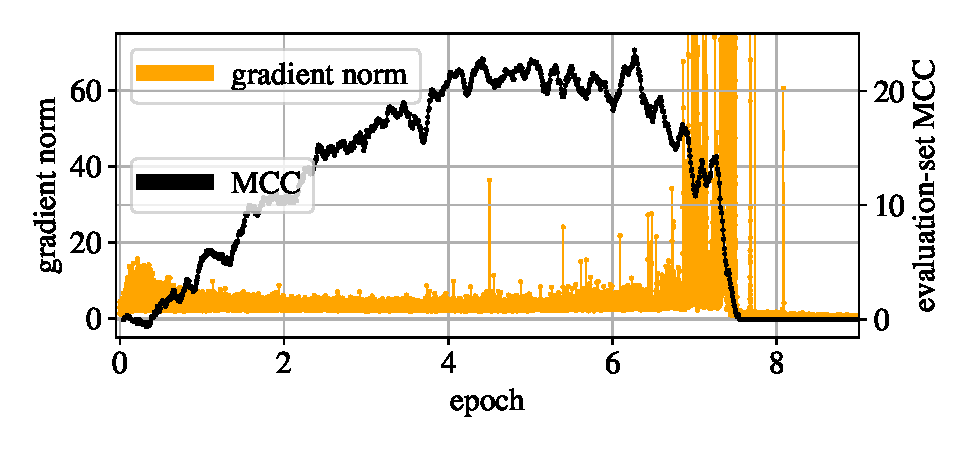
\includegraphics[width=12cm]{../experiments/analysis/img/exploding-grads.png}}
          \caption{Gradient explosion in \BERTS~with $W=2$ and $D=2$. The MCC values have been smoothed with a 0.1-epoch-wide sliding average window.}
          \label{fig:exploding-grads}
        \end{figure}

        Without further extensive exploration of optimal learning rate values for each \BERTS~size\footnote{This would be extremely time-consuming because the larger versions take over 3 days to train.}, I choose better learning rate values manually.
        Because of the use of $\eta$ warmup, I can monitor the learning progress for varying $\eta$ values in the early training epochs, as shown in \autoref{fig:exploding-grads-choosing-lr}. I approximately identify the point in training beyond which the learning slows down (and later degrades altogether) due to large gradients. This way, I approximately identify the largest learning rate that still leads to learning, not to gradient explosion. In the concrete example in \autoref{fig:exploding-grads-choosing-lr}, I choose the point in training after 2.5 epochs, where the learning rate is approximately $\eta=8\times10^{-5}$, and use this value with the concrete model size.
        
        \begin{figure}[h!t]
          \centering
          \makebox[\textwidth][c]{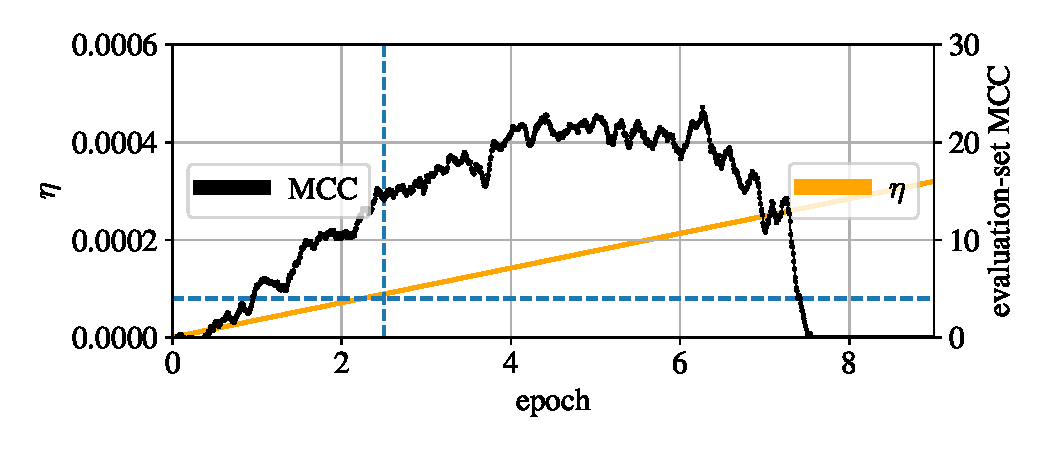
\includegraphics[width=12cm]{../experiments/analysis/img/exploding-grads-choosing-lr.png}}
          \caption{Learning progress (MCC over time) vs $\eta$ for \BERTS~with $W=2$ and $D=2$ -- the model experiencing gradient explosion in \autoref{fig:exploding-grads}. The dashed lines show the position I identify as the approximate latest point of training before the learning starts to slow down, and the learning rate at that position.
          The MCC values have been smoothed with a 0.1-epoch-wide sliding average window.}
          \label{fig:exploding-grads-choosing-lr}
        \end{figure}

        With the new learning rates manually estimated individually for each student size, none of the larger versions of \BERTS~experiences gradient explosion. The LSTM students all use the same learning rate as this does not lead to any issues. \autoref{fig:size-cola} presents the results. While some larger students outperform the original, 2.4-million-parameter ones, the trends are not consistent. For \LSTMS~in particular, there is no clear correlation between student width or depth and the performance. For \BERTS, which starts as a relatively deep model with 5 layers, making it wider rather than deeper is helpful. For \LSTMS~which originally has only 1 hidden LSTM layer, increasing both the width and the depth can lead to better-performing models. Overall, both student architectures reach the best evaluation score of \mytilde45, far below the teacher performance level of 59.9. 

        \begin{figure}
          \centering
          \begin{subfigure}{.5\textwidth}
            \centering
            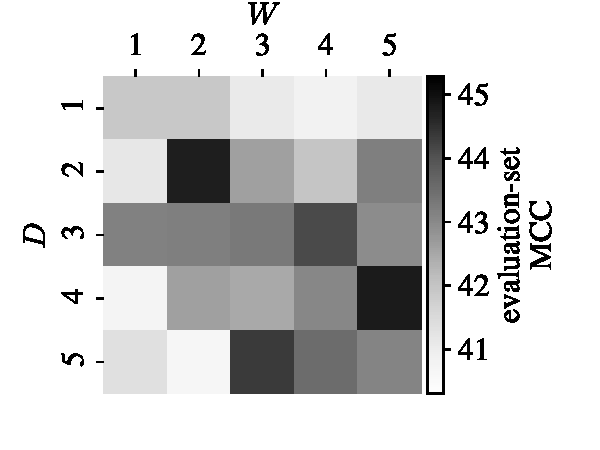
\includegraphics[width=7cm]{../experiments/analysis/img/size-cola-lstm-map}
            \caption{Different sizes of \LSTMS.}
            \label{fig:size-cola-lstm}
          \end{subfigure}%
          \begin{subfigure}{.5\textwidth}
            \centering
            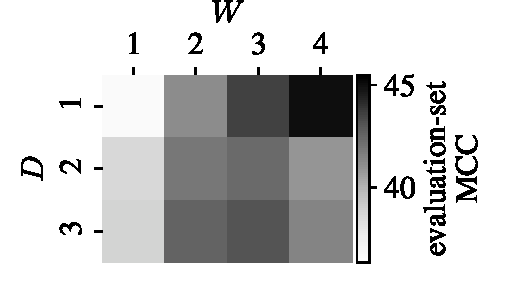
\includegraphics[width=6.5cm]{../experiments/analysis/img/size-cola-bert-map}
            \caption{Different sizes of \BERTS.}
            \label{fig:size-cola-bert}
          \end{subfigure}
          \caption{Best evaluation-set performance for the different student sizes on CoLA.}
          \label{fig:size-cola}
        \end{figure}
        
        I refrain from exploring students even larger as the biggest students are already approching the teacher size: \LSTMS~with $W=5$, $D=5$ has \mytilde247 million parameters and takes over 60h to train, and \BERTS~with $W=4$, $D=3$ has \mytilde114 million parameters and takes over 6 days to train.
        As the best-performing students, I establish \BERTS~with $W=4$, $D=1$, and \LSTMS~with $W=2$, $D=2$.
      }

      \subsubsection{SST-2}{
        As previously observed, on SST-2, even the default 2.4-million-parameter students perform on par with the teacher. With no reason to try larger student sizes, I limit myself to exploring smaller student architectures, with the aim of keeping student accuracy above 90\% of the teacher's score. With \BERTT~achieving 91.5\% accuracy, the 90\% lower bound is at \mytilde82\% accuracy.

        \autoref{fig:size-sst-2} shows that accuracy stays high even for very small students. 
        The smallest tried LSTM student ($W=1/64$, 24,360 non-embedding parameters, \mytilde14,000x smaller than \BERTT) still achieves 89.1\% accuracy (\mytilde97\% of the teacher's performance).
        The smallest tried BERT student ($W=1/16$, $D=1/4$, 2272 non-embedding parameters, \mytilde150,000x smaller than \BERTT) achieves 83.5\% accuracy (\mytilde91\% of \BERTT's performance).
        What these results mean is that the SST-2 task is relatively easy. 
        For good accuracy levels, a very minimalistic classifier is sufficient on top of the pre-trained embeddings -- the representations obtained simply by encoding each word using word2vec already contain most of the knowledge needed to make good sentiment predictions.

        \begin{figure}
        \makebox[\linewidth][c]{%
          \centering
          \begin{subfigure}{.61\textwidth}
            \centering
            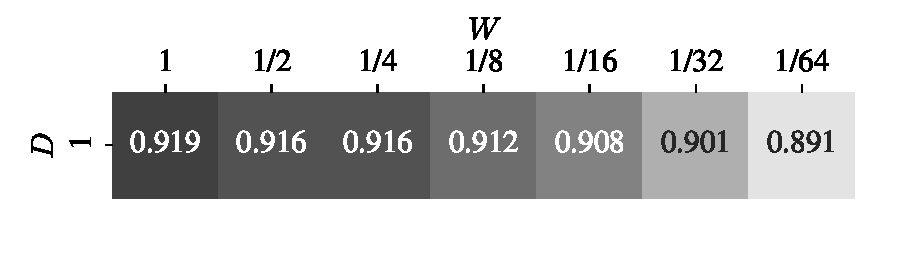
\includegraphics[width=9cm]{../experiments/analysis/img/size-sst-2-lstm-map}
            \caption{Different sizes of \LSTMS.}
            \label{fig:size-sst-2-lstm}
          \end{subfigure}%
          \begin{subfigure}{.5\textwidth}
            \centering
            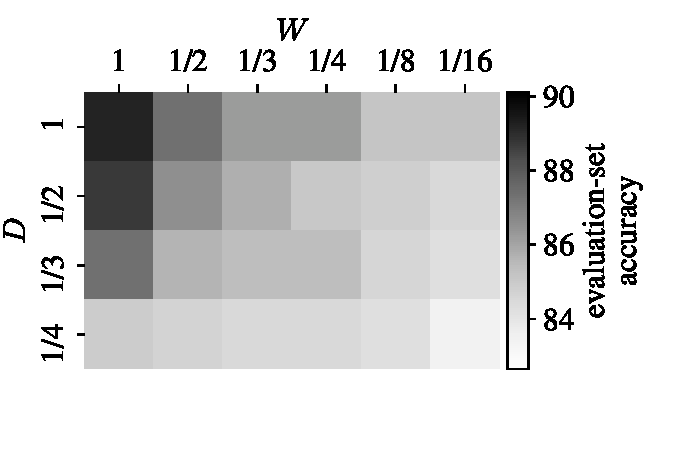
\includegraphics[width=7.5cm]{../experiments/analysis/img/size-sst-2-bert-map}
            \caption{Different sizes of \BERTS.}
            \label{fig:size-sst-2-bert}
          \end{subfigure}
        }
        \caption{Best evaluation-set performance for the different student sizes on SST-2.}
        \label{fig:size-sst-2}
        \end{figure}
        Another insight from \autoref{fig:size-sst-2-bert} is that making \BERTS~shallower affects the performance much less than making it slimmer. In other words, the 2.4-million-parameter \BERTS~may be unnecessarily deep for the task, but it is not unnecessarily wide.
      }

      \subsubsection{Sara}{
        Similar to SST-2, Sara is an easy task. With \BERTT~achieving $F_{1 micro}=87.5$, the 2.4-million-parameter \BERTS~and \LSTMS~already achieve 87.1 and 86.5, respectively.
        I further down-scale the students, see \autoref{fig:size-sara}. Similar to the results on SST-2, both students can be made much smaller while achieving over 90\% of \BERTT's performance.
        The second smallest tried \LSTMS~($W=1/4$) is 262x smaller than the teacher while retaining almost 95\% of its performance.
        The \BERTS~with $W=1/2$ and $D=1/4$, being 2500x smaller than \BERTT, retains \mytilde93\% of its performance.

        Also similarly to SST-2, making \BERTS~shallower has much weaker effect on the performance than making it thinner. In other words, the Sara task does not require very deep models, and keeping the representation dimensionality above certain level (in this case around 128 or above, corresponding to $W\geq1/2$) is more important.
        \begin{figure}
        \makebox[\linewidth][c]{%
          \centering
          \begin{subfigure}{.61\textwidth}
            \centering
            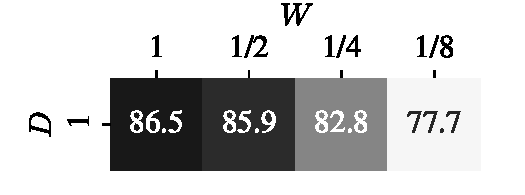
\includegraphics[width=5.4cm]{../experiments/analysis/img/size-sara-lstm-map}
            \caption{Different sizes of \LSTMS.}
            \label{fig:size-sara-lstm}
          \end{subfigure}%
          \begin{subfigure}{.5\textwidth}
            \centering
            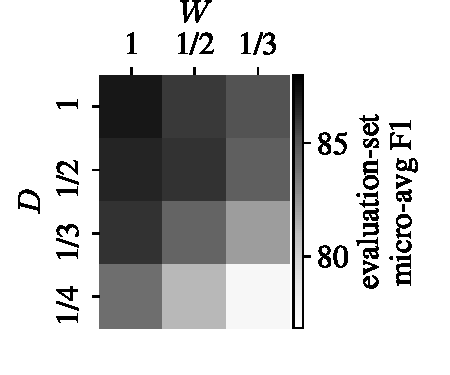
\includegraphics[width=5cm]{../experiments/analysis/img/size-sara-bert-map}
            \caption{Different sizes of \BERTS.}
            \label{fig:size-sara-bert}
          \end{subfigure}
        }
        \caption{Best evaluation-set performance for the different student sizes on Sara.}
        \label{fig:size-sara}
        \end{figure}
      }
    }
  }

  \section{Student training: conclusions}{
    % - tuning params on CoLA
    % - tuning task-secific params
    % - results: comparing best students and teachers
    By conducting a brief exploration of the students' hyper-parameters, I produced well-performing \BERTS~and \LSTMS~for each of the three downstream tasks, and gained insights into the nature of the parameters, tasks and models.

    CoLA is much more difficult of a task than SST-2 and Sara. Even with students having over 100 million parameters, they do not achieve more than 75\% of the teacher's score. Moreover, in general, \BERTS~requires more parameters than \LSTMS~for the same performance level. This can be attributed to the smaller initial width of BERT's internal representations: 204 (compare with the 300- and 400-unit layers of \LSTMS).

    There is further evidence of model width being more important than depth: In particular, the 5-layer \BERTS~can be made shallower on both SST-2 and Sara without significant performance drops. I conclude that Transformer models like the 12- and 24-layer BERTs are unnecessarily deep for tasks like intent classification or even grammatical acceptability, and making then shallower is a promising way to accelerate the models. After all, this idea is in line with \citet{Sanh_2019} who created well-performing BERT students shallower but not thinner than the teacher.

    There are several differences between \BERTS~and \LSTMS. Notably, the LSTM student converges much faster. Additionally, the much deeper BERT student is more sensitive to the learning rate values and these need to be significantly reduced for larger \BERTS~sizes. While \LSTMS~trains much faster, it works best with smaller minibatches -- if larger batch sizes worked well, the training could be sped up even further.

    The usual direction of knowledge flow into a student during knowledge distillation is top-down: Matching the teacher's logits happens at the top of the students, and gradients trickle down into the lower student layers.
    Opposite and complementary to this is the provision of trained embeddings to the early layer of a student (knowledge injected at the bottom can trickle up during further training).
    I showed that both word-level word2vec embeddings and fine-tuned wordpiece embeddings taken from \BERTT~work well with both student architectures. Importantly, certain downstream tasks like CoLA and SST-2 benefit from higher-quality word-level representations while others like Sara can benefit from the flexibility of wordpiece embeddings. It would be interesting to see how well word-level embeddings fine-tuned as part of the teacher model would perform.

    Besides leaving the embedding layer to be further trained during knowledge distillation, I observe the usefulness of keeping another -- frozen -- copy of the embeddings which reflects the initial knowledge injected before student training\footnote{This corresponds to the multichannel embedding mode.}

    \begin{table}[]
      \centering
      \fontsize{10}{11} \selectfont 
      \begin{tabular}{l|l|l|l|l|l|c|l}
       &
        model  &
        size &
        width &
        $L$ &
        $\eta$ \& scheduling &
        $B$ &
        embeddings \\
        \hline
      \multirow{2}{*}{\rotatebox[origin=c]{90}{CoLA}} &
        \BERTS &
        76.4M &
        \begin{tabular}{@{}l@{}}$d_h=816$, \\$d_I=3000$, $A=12$ \end{tabular} &
        5 &
        \begin{tabular}{@{}l@{}}$\eta=7\times10^{-5}$, \\$E_w=15$, decay\end{tabular} &
        128 &
        \begin{tabular}{@{}l@{}}word2vec,\\multichannel\end{tabular} \\
        \cline{2-8}
       &
        \LSTMS &
        15.4M &
        \begin{tabular}{@{}l@{}}$d_{LSTM}=600$,\\$d_{FC}=800$\end{tabular} &
        2 &
        \begin{tabular}{@{}l@{}}$\eta=5\times10^{-4}$, \\$E_w=0$, decay\end{tabular} &
        32 &
        \begin{tabular}{@{}l@{}}word2vec,\\multichannel\end{tabular} \\
        \hline
      \multirow{2}{*}{\rotatebox[origin=c]{90}{SST-2}} &
        \BERTS &
        2.4M &
        \begin{tabular}{@{}l@{}}$d_h=204$,\\$d_I=750$, $A=3$\end{tabular} &
        5 &
        \begin{tabular}{@{}l@{}}$\eta=5\times10^{-4}$, \\$E_w=15$, decay\end{tabular} &
        128 &
        \begin{tabular}{@{}l@{}}word2vec,\\multichannel\end{tabular} \\
        \cline{2-8}
       &
        \LSTMS &
        2.4M &
        \begin{tabular}{@{}l@{}}$d_{LSTM}=300$,\\$d_{FC}=400$\end{tabular} &
        1 &
        \begin{tabular}{@{}l@{}}$\eta=5\times10^{-4}$, \\$E_w=0$, decay\end{tabular} &
        32 &
        \begin{tabular}{@{}l@{}}word2vec,\\multichannel\end{tabular} \\
        \hline
      \multirow{2}{*}{\rotatebox[origin=c]{90}{Sara}} &
        \BERTS &
        2.4M &
        \begin{tabular}{@{}l@{}}$d_h=204$,\\$d_I=750$, $A=3$\end{tabular} &
        5 &
        \begin{tabular}{@{}l@{}}$\eta=5\times10^{-4}$, \\$E_w=15$, decay\end{tabular} &
        128 &
        \begin{tabular}{@{}l@{}}wordpiece,\\non-static\end{tabular} \\
        \cline{2-8}
       &
        \LSTMS &
        2.4M &
        \begin{tabular}{@{}l@{}}$d_{LSTM}=300$,\\$d_{FC}=400$\end{tabular} &
        1 &
        \begin{tabular}{@{}l@{}}$\eta=5\times10^{-4}$, \\$E_w=0$, decay\end{tabular} &
        32 &
        \begin{tabular}{@{}l@{}}wordpiece,\\multichannel\end{tabular} \\
      \end{tabular}
      \caption{Configuration for the best students on each task. The model size denotes the number of trainable, non-embedding parameters.}
      \label{tab:best-students}
    \end{table}

    \begin{figure}[h!tb]
      \centering
      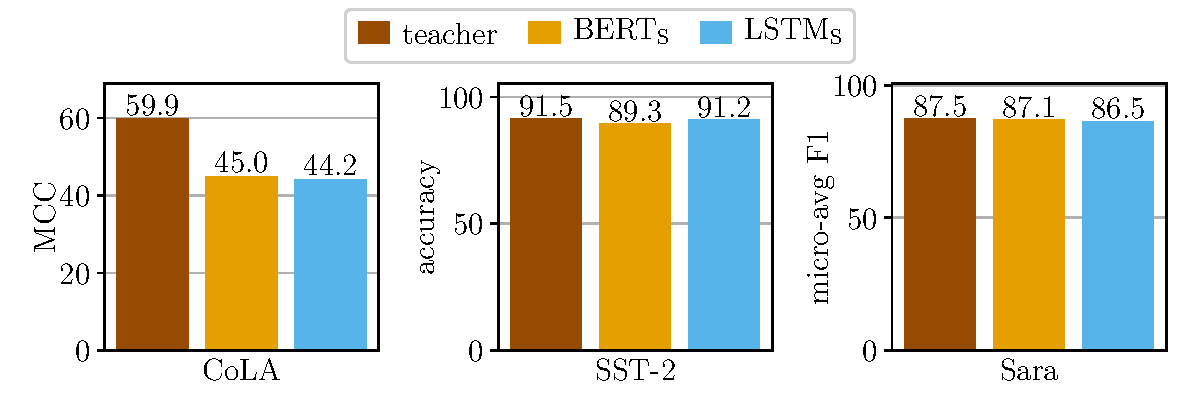
\includegraphics[width=13cm]{../experiments/analysis/img/best-models-scores.pdf}
      \caption{Evaluation-set scores of the teacher and the best students for each downstream task.}
      \label{fig:best-models-scores}
    \end{figure}

    \autoref{tab:best-students} summarises the parameters of best students on each task. These 6 students, together with their teachers, I will use for further analysis. \autoref{fig:best-models-scores} compares the best students with the teacher in terms of the evaluation-set score.
  }
}

\chapter{Analysing the models}{
  In this chapter, I use probing and prediction analysis to analyse, interpret and compare the teacher and the best student models for each downstream task. In doing so, I produce insights into the nature of the downstream tasks, the models, and knowledge distillation.

  \section{Probing \reviewready}{
    % typical pipeline (Tenney)
    \citet{Tenney_2019b} recently showed that a typical text processing pipeline can be identified in BERT. The early layers specialise in extracting simple properties like word classes (POS tags).
    Later layers extract more sophisticated information like dependencies (identifying the subject, object, and others).
    The last layers are capable of extracting complex semantic information such as real-world relations (predicting the relation between ``Mary'' and ``work'' in ``Mary is walking to work.'' to be of type \verb|Entity-Destination|\footnote{Example borrowed from \citet[p. 4]{Tenney_2019a}.}).
    
    % how the pipeline maps onto these probing tasks
    In the probing suite of \citet{Conneau_2018}, which I use, the pipeline steps are represented from the simplest ones to the most complex ones; from extracting surface properties like sentence length (\verb|Length|) and concrete input words (\verb|WordContent|), through extracting syntactic structure (\verb|Depth|, \verb|TopConstituents|), to identifying the subject, object and the main verb of a sentence and their properties (\verb|Tense|, \verb|SubjNumber|, \verb|ObjNumber|), to detecting broken semantics (\verb|OddManOut|, \verb|CoordinationInversion|).

    % observing the knowledge flow: pretrained > fine-tuned > distilled
    The probing suite itself is a tool which can be used in various ways. I use it primarily to trace language knowledge, to observe how the pre-trained knowledge of BERT is retained or changed in teacher fine-tuning, and subsequently distilled into student models.
    % measuring total amount AND localising
    While \citeauthor{Conneau_2018} apply probing only to the final representations extracted from various sentence encoders, I adopt the approach of \citeauthor{Tenney_2019b} and probe models at different layers. Thus, I not only quantify the linguistic knowledge, but also localise it within a given model\footnote{As discussed in \autoref{sec:implementation-details-probing}, in the case of \LSTMS, I am only able to probe the final representations due to the way LSTMs are implemented in PyTorch.}.
    
    % differences across models: tells something about KD into different architctures and what students don't learn
    By analysing the differences in lingustic knowledge between \BERTT, \BERTS, and \LSTMS~on a particular downstream task, I explore the effects of different student architectures as well as the kinds of knowledge that is easy or difficult for the students to learn.
    % differences across tasks: what linguistic capabilities are useful
    By observing differences between models trained on different downstream tasks, I explore the possibility of characterising a downstream task by the kinds of linguistic knowledge it does or does not require.

    \subsection{Probing teacher models}{
      \autoref{fig:probing-teachers} compares the probing results of the pre-trained BERT and of BERT further fine-tuned on different downstream tasks.
      % pre-trained similar to fine-tuned
      First of all, the results are mostly very similar across all the models, which means that fine-tuning on downstream tasks did not change the models too drastically.

      % all models deviate in late layers (most fine-tuning happens there, early layers are universal feature extractors and perhaps could be frozen)
      The models's results deviate especially for the last layers while for early layers fine-tuning does not lead to any changes. In other words, only the last model layers get fine-tuned to the particular tasks, while the early layers effectively act as extractors of univerally usable features. (It is therefore likely that the teacher models could be fine-tuned well even with the early layers frozen or only allowed to change during a small portion of the fine-tuning steps, thus making the fine-tuning faster.)

      % fine-tuned knowledge replaces pre-trained when not needed: evident with CoLA which doesn't throw linguistic knowledge away (Sara does, and SST-2 does even more so)
      Another way of thinking about the teacher fine-tuning is that the pre-trained language knowledge is ``replaced'' by downstream task-specific skills. If the downstream task relies on the linguistic skills, then they are retained.
      This effect is clear in \autoref{fig:probing-teachers} when comparing the CoLA teacher with the SST-2 and Sara ones. As a task about linguistic acceptability, CoLA requires models to be sensitive to a wide range of linguistic principles and their violations. Therefore, very little of the pre-trained language knowledge is lost in fine-tuning -- on the \verb|BigramShift| task, the CoLA \BERTT~even outperforms the pre-trained model. Sentiment classification, on the other hand, requires capabilities very different from typical linguistic skills, leading to the last layers of the SST-2 \BERTT~retaining little of the pre-trained skills. Intent classification leads to retaining some of the pre-trained knowledge; arguably, skills like distinguishing between greetings, statements, commands and questions, or understanding that two sentences are semantically equivalent, are desirable for a task like Sara.

      Interestingly, on \verb|WordContent|, the CoLA teacher ``forgets'' more than the Sara teacher. I explain this in terms of certain Sara intents strongly linked to specific words -- for example, examples of the intent \verb|affirm| mostly identified by their use of ``yes'' or ``okay''. Therefore, a good model for Sara will likely ``remember'' the exact input words even in higher layers.

      \begin{figure}[h!tb]
        \centering
        \makebox[\textwidth][c]{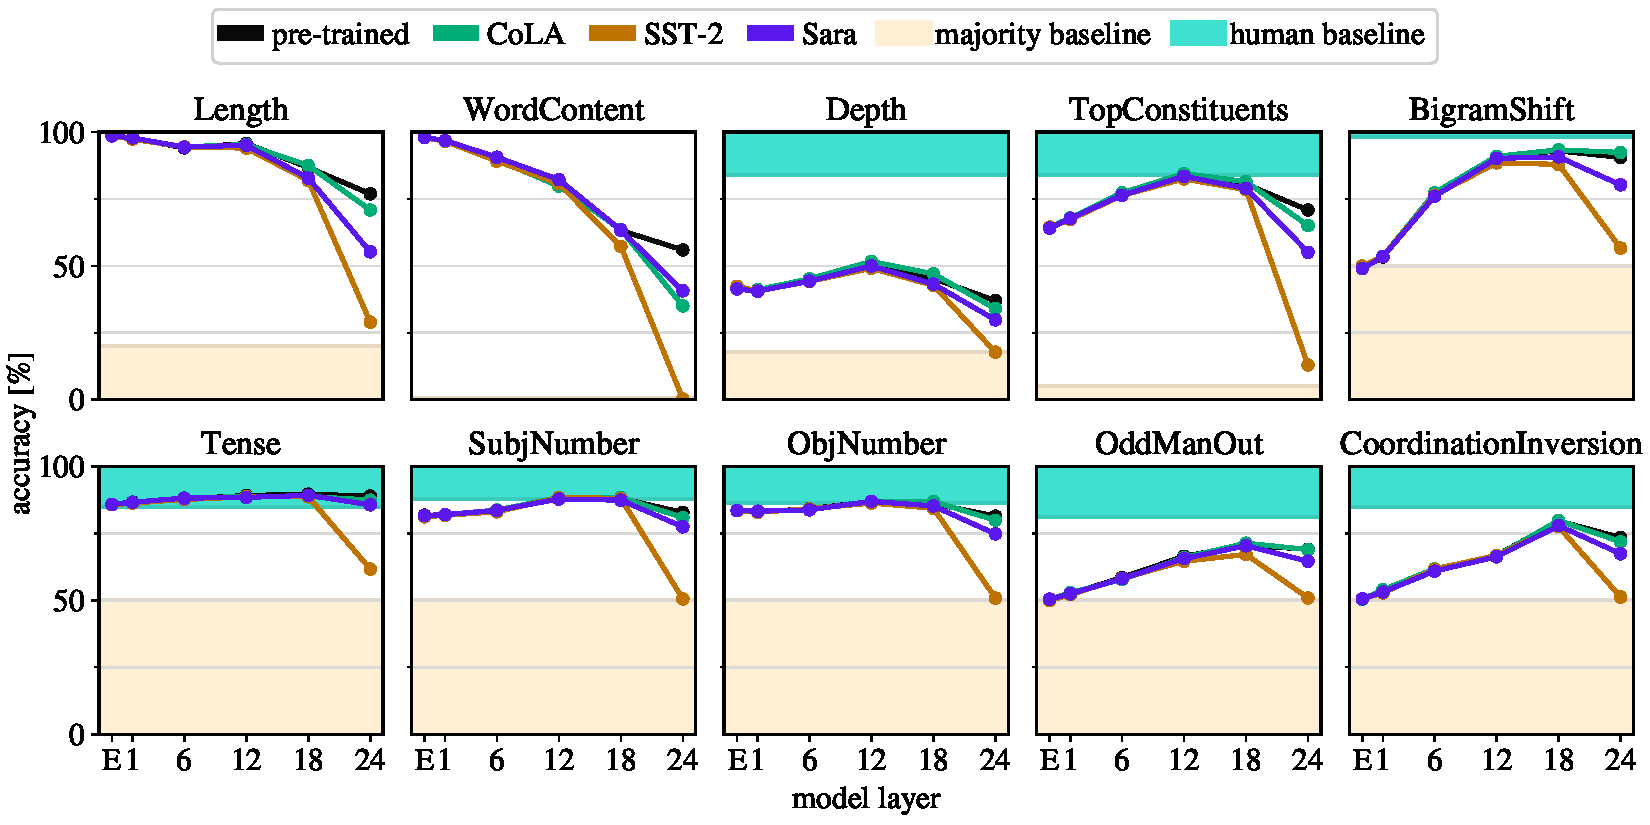
\includegraphics[width=17cm]{../experiments/analysis/img/probing_teachers.pdf}}
        \caption{Probing results for the pre-trained BERT and the teacher BERT models. Probing was applied to encoder layers 1, 6, 12, 18, and 24, and to the embeddings (layer ``E'') extracted just before the first encoder layer. The two baselines, bounding the expected model performance from below and from above, are the majority-class baseline and the human performance baseline as reported by \citet{Conneau_2018}.}
        \label{fig:probing-teachers}
      \end{figure}

      % tasks localised mostly nicely and as expected (length, WC, depth and TC, SOMO and CI). BS also semantic! tense, SN, ON possible since E layer (morphology), syntax slightly improves.
      Last but not least, the curves for each probing task in \autoref{fig:probing-teachers} show how different linguistic skills are localised in the usual way. The two surface property skill (\verb|Length|, \verb|WordContent|) are localised in the first layers which have access to the input. The syntactic skills -- \verb|Depth| and \verb|TopConstituents| -- are localised in the middle layers. Finally, the semantic tasks -- \verb|OddManOut| and \verb|CoordinationInversion| are best handled by the last layers.
      
      An interesting case is the \verb|BigramShift| task which, as previously discussed, is both syntactic and semantic, because disturbing the word order in a sentence typically disrupts both the meaning and the sentence structure structure. As a result, this probing task is handled well by the middle layers as well as the later ones.
      
      As for \verb|Tense|, \verb|SubjNumber| and \verb|ObjNumber|, they are handled well by all layers, but by the later ones in particular. I hypothesise that the overall good performance is due to the morphological component of the tasks. Statistically, in most cases, the tense of the main verb in English can be determined just by checking if a word in the sentence ends with ``-d/-ed'' (the regular-verb past tense marker) or not. Similarly, the number of the subject or object can be guessed just from knowing if any word ends in ``-s'' (the plural marker). Since morphological knowledge is known to be contained in pre-trained embeddings, even the embedding layer output performs well on these tasks. Minor improvements can be made by considering semantic and syntactic knowledge in cases where it is important to know which word of the sentence is the object, subject or main verb, or in cases where the markers are unusual (irregular verbs, unusual plural forms or singular forms ending in ``-s''). This is in line with the later layers performing slightly better than the early ones.
    }

    \subsection{Probing student models}{
      \autoref{fig:probing-students} shows the results of probing the best \LSTMS~and \BERTS~for each downstream task. To put the scores into perspective, I also include results achieved by probing the students' embeddings \textit{before} student training: This means pre-trained word2vec embeddings for CoLA and SST-2\footnote{As previously discussed, only the embeddings corresponding to words found in the transfer dataset are taken.}, and wordpiece embeddings from \BERTT~for Sara.
      
      \begin{figure}[h!tb]
        \centering
        \makebox[\textwidth][c]{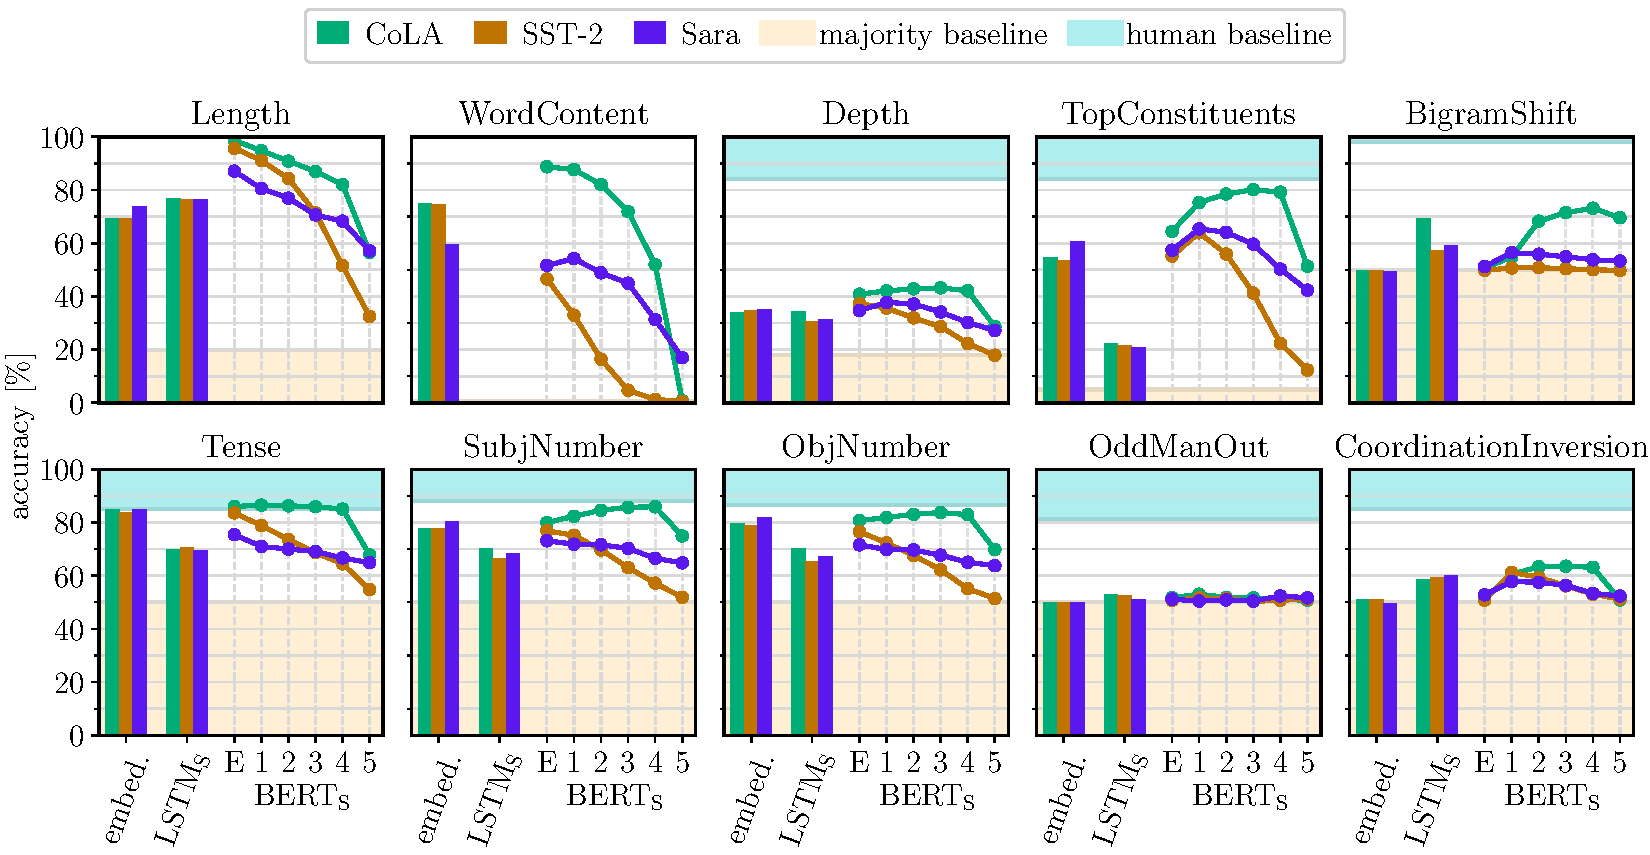
\includegraphics[width=17.5cm]{../experiments/analysis/img/probing_students.pdf}}
        \caption{Probing results for the best student models. For comparison, results achieved just by using embeddings are shown as well (labelled ``embed.''). While for \LSTMS, the probing encodings were extracted only after the last LSTM layer, for \BERTS, I extracted encodings after each of the 5 encoder layers and embedding encodings from before the first layer (labelled ``E''). Bounding the expected model performance from below and from above are again the majority-class baseline and the human performance baseline, same as in \autoref{fig:probing-teachers}.}
        \label{fig:probing-students}
      \end{figure}

      % comparing students with teacher:
      % - student takes much knowledge from embeddings whereas entire teacher is pre-trained: hence, in student probing scores typically go down from E to last layer whereas in teacher only in last layers there's a drop
      % - similar teacher-bert end points: Length (except CoLA), Depth, TC, 
      % - bert student worse: BS, Tense, ONum, SNum, SOMO, CI
      The first significant difference when comparing \autoref{fig:probing-students} with \autoref{fig:probing-teachers} is the progressive decrease in probing scores of \BERTS~from earlier to later layers (in \BERTT, the scores only fall in the last layers). This is mostly visible in \autoref{fig:probing-students} for \verb|Length|, \verb|WordContent|, \verb|Tense|, \verb|SubjNumber| and \verb|ObjNumber|. 
      The decreasing scores reflect the different ways in which \BERTT~and \BERTS~are initialised. The teacher starts with all layers pre-trained (i.e. containing general language knowledge). During teacher fine-tuning, it is the last layer through which feedback enters the model. Therefore, the language knowledge is disturbed mostly in the last layers.
      The students, on the other hand, start with pre-trained knowledge ``injected'' only from the bottom -- in the embedding layer. During student training (knowledge distillation), learning feedback enters from the top (in the last layer), but, at the same time, the embedding knowledge propagates up, affecting the earliest layers the most.
      Thus, the decreasing probing scores can be interpreted as markers of linguistic knowledge which was present in the initial embeddings, but the model did not retain it in the later layers. Either the knowledge was not needed for the downstream task, or the knowledge was only useful in creating more general representations in the first layers.
      % Lesson: trace the initial knowledge, it's important!

      In general, both students perform worse than the respective teachers on all probing tasks. This is not surprising as the students are smaller and lack the pre-trained knowledge that the teachers contain before fine-tuning. The students underperform especially on three tasks: \verb|BigramShift|, \verb|OddManOut|, and \verb|CoordinationInversion|. These are difficult tasks, not solvable just using embeddings (in \autoref{fig:probing-students}, the embeddings perform at the bottom baseline level). In other words, the students need to learn these linguistic skills by themselves, which they do with mixed success; in particular, all students fail to recognise semantically disturbed sentences in \verb|OddManOut|.
      % Lesson: Students naturally underperform; focus on bits they can successfully learn by themselves.

      % comparing same student across tasks:
      % - small differences in LSTM (interesting; could mean that LSTM being shallower is a more universal feature extractor and the FC hat is task-specific); only exception BS for CoLA -- crucial, as observed with teachers
      % - CoLA BERT clearly says that Depth, TC, BS, Tense, SNum, ONum and CI are important for CoLA
      % - as previously, SST-2 loses language knowledge the most
      Comparing the probing scores of one student architecture trained on different downstream tasks, there are several important observations.
      Firstly, different instances of \LSTMS~perform similarly. This is likely due to the student being shallow, therefore the LSTM layer(s) producing relatively similar, task-agnostic representations, and only the fully-connected layer being heavily task-specific.
      Secondly, the CoLA task clearly encourages \BERTT~to learn a wide range of linguistic knowledge (much more strongly than for SST-2 and Sara): be it syntax (\verb|Depth|, \verb|TopConstituents|, \verb|BigramShift|), morphology and dependencies (\verb|Tense|, \verb|SubjNumber|, \verb|ObjNumber|), or semantics (\verb|BigramShift|, \verb|CoordinationInversion|).
      Thirdly, as previously observed for different teachers, SST-2 requires the least linguistic knowledge and typically leads to the lowest probing scores.
      % Lesson: shallow models focus on general features. CoLA requires various linguistic skills.

      % comparing two students:
      % - LSTM comparable with last BERT layer: BS, SOMO, WC
      % - LSTM comparable with middle layers: Length, Depth, Tense,
      % - LSTM just worse: TC
      When comparing the two student architectures trained on the same downstream tasks, it is difficult to observe any clear trends.
      \LSTMS~performs comparably with the last \BERTS~layers (\verb|BigramShift|, \verb|WordContent|, \verb|OddmanOut|), on some other tasks \LSTMS~roughly compares to the middle layers of \BERTS~(\verb|Length|, \verb|Depth|, \verb|Tense|), and still other times \LSTMS~performs much worse than any layers of \BERTS~(\verb|TopConstituents| for CoLA and Saras).
      On \verb|WordContent|, \LSTMS~fails altogether, compared with \BERTS. This may be due to the residual connections in BERT, which enable easy copying of input tokens across layers, while LSTM has no such bypass mechanism.
      Overall, only in few cases, \LSTMS~outperforms any of \BERTS's layers. This happens on most probing tasks in the case of SST-2, where the last layers of \BERTS~lose practically all linguistic knowledge.
      Interestingly, in the case of SST-2 and Sara, \LSTMS~outperforms \BERTS~on \verb|BigramShift| and \verb|CoordinationInversion| -- the two probing tasks that require sensitivity to word and clause order. It may be due to the recurrent nature of \LSTMS~which makes such order sensitivity an inherent property of the model. The recurrent student is also more sensitive to overall input length.
      % Lesson: Hard to tell if LSTM is worse than BERT but often it is. LSTM does well on order and length tasks because of its architecture.

      % comparing students with embed:
      % - LSTM worse on embedding tasks: WC, Tense, SubNum, ObjNum
      % - BERT E roughly at embed level (understandable, not much changes to embeddings during KD), Length and WC being only exceptions
      Relative to the probing results of the embeddings taken before knowledge distillation (see ``embed.'' in \autoref{fig:probing-students}), the students sometimes perform better and other times worse. In the morphology-oriented tasks which use a lot of embeding knowledge (\verb|Tense|, \verb|SubjNumber|, \verb|ObjNumber|), \LSTMS~understandably performs worse than the embeddings and similar to the last layers of \BERTS. The embeddings from the trained \BERTS~achieve mostly comparable probing results, signalling that they did not change much during the student training (in line with the argument that the top layers change the most).
      % Lesson: Nothing too important, knowledge propagates from embeddings.
      
      % localisation: may be hard because many skills seemingly localised before first layer (just because embeddings!): Length, WC, Tense, SNum, ONum.
      % - true localisation: non-embedding skills (>= 1 layer of precessing): Depth, TC, BS, CI; in late layers: Depth, TC, BS, SNum, ONum, CI
      Localising different linguistic knowledge is possible in \BERTS\footnote{Because I probed only one layer of \LSTMS, there, localising knowledge is not possible.}. Many skills are, at the first sight, concentrated in and before for first layer (\verb|Length|, \verb|WordContent|, \verb|Tense|, \verb|SubjNumber|, \verb|ObjNumber|), but in most cases this is likely an artifact of the embeddings being the initial source of this knowledge. In other cases, knowledge in \BERTS~is clearly concentrated in higher layers (for CoLA on tasks \verb|TopConstituents|, \verb|BigramShift|, \verb|SubjNumber|, \verb|ObjNumber|, \verb|CoordinationInversion|). Interesting is the syntactic task \verb|TopConstituents|, where going from the ``E'' layer to layer 1 in all \BERTS~students increases the probing score significantly. In other words, the trained embeddings contain the necessary knowledge, but at least one model layer is required to aggregate and combine the knowledge across input tokens into sentence-level structural knowledge needed for the task.
    }

    \subsection{What can students learn from scratch}{
      In the previous section, I observed how language knowledge enters student models from the provided pre-trained embeddings. Naturally, such ``intruder'' knowledge makes it difficult to interpret probing scores of students. In particular, does a high score mean that the student acquired the skill in question during training, or was the knowledge merely present in the injected embeddings?

      To control for the initial knowledge present in a student, I probe students trained from scratch, i.e. with embeddings initialised randomly the same way as the rest of the models. In general, the probing results do not differ much from those of students initialised with pre-trained embeddings. In particular, the differences are very small for \LSTMS, which is understandable -- I probe the model after its last LSTM layer, whereas injecting pre-trained knowledge tends to affect the first layers. For \BERTS, the variant initialised from scratch often performs slightly worse, which is again understandable given the lack of initial knowledge.

      \begin{figure}[h!tb]
        \centering
        \makebox[\textwidth][c]{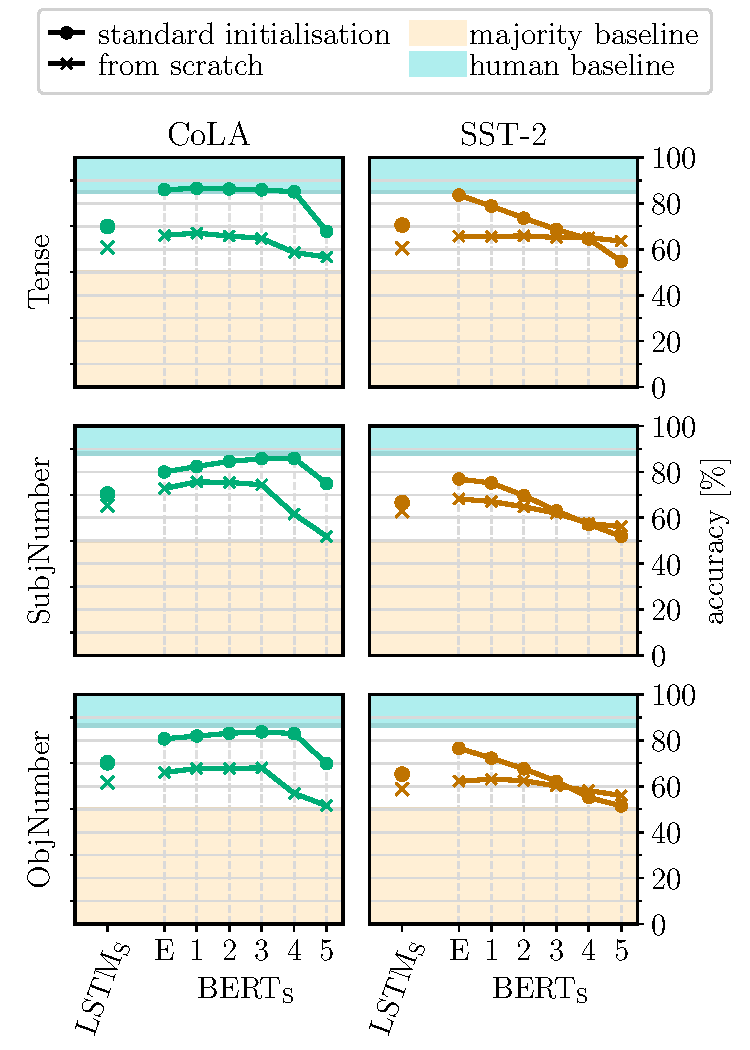
\includegraphics[width=9.5cm]{../experiments/analysis/img/probing_students_scratch_selected.pdf}}
        \caption{Probing results for selected downstream and probing tasks, comparing studentss initialised in the standard way (with embeddings from word2vec) with students initialised randomly and trained from scratch. Bounding the expected model performance from below and from above are again the majority-class baseline and the human performance baseline, same as in \autoref{fig:probing-teachers}.}
        \label{fig:probing-students-scratch-selected}
      \end{figure}

      In \autoref{fig:probing-students-scratch-selected} I show the most striking differences (for full results see \autoref{chap:A-probing}). Namely, for \BERTS~trained on CoLA and SST-2, on the three probing tasks which I previously described as morphology-oriented and to a great extent relying on embedding knowledge: \verb|Tense|, \verb|SubjNumber|, and \verb|ObjNumber|.
      Without pre-trained embeddings, all layers of the CoLA \BERTS~perform much worse on these probing tasks. While these linguistic skills are arguably important for a task like CoLA, it is clear that the student is unable to learn them well without the embedding knowledge provided beforehand.
      In the case of the SST-2 student, the original probing scores show progressive decay of performance from earlier to later layers. This, as I previously discussed, can be attributed to the relevant knowledge propagating form the pre-trained embeddings up through the model during training. When the pre-trained knowledge is initially absent, as \autoref{fig:probing-students-scratch-selected} shows, the decay effect is weak or not present at all. Instead, all layers alike achieve low probing scores. This is a strong signal that the morphology-oriented skills were not needed for the Sara task, and so \BERTS~did not learn them well.

      All in all, this simple experiment showed that probing results should be interpreted very carefully. In particular, if a model achieves a high probing score, it may be due to different reasons:
      \begin{itemize}
        \item The model as such was pre-trained, with language knowledge present before the task-specific training (like in the case of \BERTT).
        \item The model may have received the knowledge (or a large part of it) when its embedding layer was initialised with trained parameters.
        \item The knowledge may be needed for the task the model is trained to do, and the model actively acquired the knowledge from the data during its training.
      \end{itemize}
    }
  }

  % analysing mistakes, probing
  \section{Analysing the models' predictions}{
    This will involve for each downstream task:
    \begin{enumerate}
      \item gathering dev-set predictions made by the two best students and the teacher
      \item looking at the mistakes made by each model (most confident mistakes and least confident mistakes first, maybe taking first 10-20 mistakes from each end), trying to describe then in intuitive terms if possible
      \item comparing the mistakes made by different models, again trying to describe what I observe
      \item looking at how confident the predictions were in general for each model (maybe the distribution of confidences?) and if possible, comparing this across models
    \end{enumerate}

    My aim is to make at least some observations describable in human-understandable terms about how the models compare: how the 2 architecturally different students compare, and how their predicting behaviour compares to that of their teacher.
    Ideally, I will be also able to form some (even if weak) hypotheses that are further testable using probing tasks.
  }
}

\chapter{Overall discussion and conclusions}{
  
}

\chapter{Future work}{
  
}

\bibliographystyle{apalike}
\bibliography{s1513472-minf2}

\appendix
\chapter{Sara dataset}{
  \label{chap:A-Sara}
  \begin{center}
    \begin{longtable}{p{0.3\textwidth}|p{0.4\textwidth}|p{0.3\textwidth}}
    \hline
    intent name & description & example \\ 
    \hline
    \endfirsthead
    
    \hline
    \multicolumn{3}{c}%
    {\tablename\ \thetable\ -- \textit{Continued from previous page}} \\
    \hline
    \endhead

    \hline 
    \multicolumn{3}{r}{\textit{Continued on next page}} \\
    \endfoot
    \endlastfoot

    \begin{spverbatim}affirm\end{spverbatim} & affirmative response & \begin{spverbatim}yes please!\end{spverbatim} \\
    \hline
    \begin{spverbatim}ask_builder\end{spverbatim} & asking Sara who built her & \begin{spverbatim}who developed you\end{spverbatim} \\
    \hline
    \begin{spverbatim}ask_faq_channels\end{spverbatim} & asking Sara about the messaging channels that Rasa tools support & \begin{spverbatim}what chat channels does rasa uses\end{spverbatim} \\
    \hline
    \begin{spverbatim}ask_faq_community_size\end{spverbatim} & asking Sara about the size of the Rasa contributor community & \begin{spverbatim}Is the community large?\end{spverbatim} \\
    \hline
    \begin{spverbatim}ask_faq_
    differencecorenlu\end{spverbatim} & asking Sara about the difference between two major components of the Rasa tools: Rasa NLU and Rasa Core & \begin{spverbatim}what is the difference between core and nlu?\end{spverbatim} \\
    \hline
    \begin{spverbatim}ask_faq_languages\end{spverbatim} & asking Sara about the languages supported by Rasa tools & \begin{spverbatim}do you support french ?\end{spverbatim} \\
    \hline
    \begin{spverbatim}ask_faq_opensource\end{spverbatim} & asking Sara if Rasa products are open source & \begin{spverbatim}are you full open source\end{spverbatim} \\
    \hline
    \begin{spverbatim}ask_faq_platform\end{spverbatim} & asking Sara about the Rasa Platform product & \begin{spverbatim}tell me what is platform\end{spverbatim} \\
    \hline
    \begin{spverbatim}ask_faq_python_version\end{spverbatim} & asking Sara about the version of Python supported by Rasa tools & \begin{spverbatim}which python version\end{spverbatim} \\
    \hline
    \begin{spverbatim}ask_faq_slots\end{spverbatim} & asking Sara about \textit{slots}, a concept in Rasa tools for holding human-provided contextual information during conversations & \begin{spverbatim}what do you mean by slots?\end{spverbatim} \\
    \hline
    \begin{spverbatim}ask_faq_tutorials\end{spverbatim} & asking Sara about tutorials on using Rasa tools & \begin{spverbatim}is there a tutorial for this?\end{spverbatim} \\
    \hline
    \begin{spverbatim}ask_faq_voice\end{spverbatim} & asking Sara about the possibility to create a voice assistant using Rasa & \begin{spverbatim}you have speech recognition?\end{spverbatim} \\
    \hline
    \begin{spverbatim}ask_faq_what_is_forum\end{spverbatim} & asking Sara about the online Rasa community forum & \begin{spverbatim}what can I post in the forum?\end{spverbatim} \\
    \hline
    \begin{spverbatim}ask_how_contribute\end{spverbatim} & asking Sara how one can contribute to the Rasa open-source project & \begin{spverbatim}How can I add code to Rasa\end{spverbatim} \\
    \hline
    \begin{spverbatim}ask_howbuilt\end{spverbatim} & asking Sara how she was built & \begin{spverbatim}so how were you made?\end{spverbatim} \\
    \hline
    \begin{spverbatim}ask_howdoing\end{spverbatim} & asking Sara how she is doing & \begin{spverbatim}Hows it going\end{spverbatim} \\
    \hline
    \begin{spverbatim}ask_howold\end{spverbatim} & asking Sara about her age & \begin{spverbatim}do you know how old you are?\end{spverbatim} \\
    \hline
    \begin{spverbatim}ask_isbot\end{spverbatim} & asking Sara if she is a bot & \begin{spverbatim}are you really a bot\end{spverbatim} \\
    \hline
    \begin{spverbatim}ask_languagesbot\end{spverbatim} & asking Sara about the languages she can speak & \begin{spverbatim}how many languages are you fluent in?\end{spverbatim} \\
    \hline
    \begin{spverbatim}ask_question_in_forum\end{spverbatim} & asking Sara a question about the Rasa community forum & \begin{spverbatim}how can I leave a query in the forum?\end{spverbatim} \\
    \hline
    \begin{spverbatim}ask_restaurant\end{spverbatim} & asking Sara to recommend a restaurant & \begin{spverbatim}Where should I eat?\end{spverbatim} \\
    \hline
    \begin{spverbatim}ask_time\end{spverbatim} & asking Sara about the time & \begin{spverbatim}tell me the time it is.\end{spverbatim} \\
    \hline
    \begin{spverbatim}ask_weather\end{spverbatim} & asking Sara about the weather & \begin{spverbatim}excellent - is it hot in Berlin?\end{spverbatim} \\
    \hline
    \begin{spverbatim}ask_whatismyname\end{spverbatim} & asking Sara to tell the person's name & \begin{spverbatim}can you tell me my name?\end{spverbatim} \\
    \hline
    \begin{spverbatim}ask_whatisrasa\end{spverbatim} & asking Sara what Rasa is & \begin{spverbatim}OK can u brief me Abt rasa\end{spverbatim} \\
    \hline
    \begin{spverbatim}ask_whatspossible\end{spverbatim} & asking Sara about the things she can do/help with & \begin{spverbatim}how u can help me\end{spverbatim} \\
    \hline
    \begin{spverbatim}ask_when_next_event\end{spverbatim} & asking Sara about the next scheduled Rasa community event & \begin{spverbatim}what date is the next community event?\end{spverbatim} \\
    \hline
    \begin{spverbatim}ask_wherefrom\end{spverbatim} & asking Sara where she is from & \begin{spverbatim}where did you grow up?\end{spverbatim} \\
    \hline
    \begin{spverbatim}ask_which_events\end{spverbatim} & asking Sara about the current Rasa community events & \begin{spverbatim}what sort of social events are we throwing?\end{spverbatim} \\
    \hline
    \begin{spverbatim}ask_whoami\end{spverbatim} & asking Sara who the human person is & \begin{spverbatim}tell me who I am?\end{spverbatim} \\
    \hline
    \begin{spverbatim}ask_whoisit\end{spverbatim} & asking who is it (like on the phone) & \begin{spverbatim}who am i talking to\end{spverbatim} \\
    \hline
    \begin{spverbatim}ask_why_contribute\end{spverbatim} & asking Sara about the reasons to contribute to Rasa & \begin{spverbatim}Why should I contribute to your code?\end{spverbatim} \\
    \hline
    \begin{spverbatim}bye\end{spverbatim} & ending a conversation with Sara by saying bye & \begin{spverbatim}take care\end{spverbatim} \\
    \hline
    \begin{spverbatim}canthelp\end{spverbatim} & telling Sara she cannot help with what is needed & \begin{spverbatim}i guess you can't help me then\end{spverbatim} \\
    \hline
    \begin{spverbatim}contact_sales\end{spverbatim} & asking Sara about ways to contact the Rasa sales team & \begin{spverbatim}i want to talk to sales\end{spverbatim} \\
    \hline
    \begin{spverbatim}deny\end{spverbatim} & provide a negative, denying response to Sara & \begin{spverbatim}no sorry\end{spverbatim} \\
    \hline
    \begin{spverbatim}enter_data\end{spverbatim} & providing information asked for by Sara & \begin{spverbatim}the assistant is in dutch\end{spverbatim}, or \begin{spverbatim}my name is __PERSON_NAME__\end{spverbatim} \\
    \hline
    \begin{spverbatim}greet\end{spverbatim} & saying hi to Sara & \begin{spverbatim}hey let's talk\end{spverbatim} \\
    \hline
    \begin{spverbatim}handleinsult\end{spverbatim} & telling an insult to Sara & \begin{spverbatim}i hate your dumb face\end{spverbatim} \\
    \hline
    \begin{spverbatim}how_to_get_started\end{spverbatim} & asking Sara how one can get started with Rasa tools & \begin{spverbatim}how to build a chatbot\end{spverbatim} \\
    \hline
    \begin{spverbatim}human_handoff\end{spverbatim} & asking to be put through to a human instead of the Sara bot & \begin{spverbatim}let me speak with a real person please\end{spverbatim} \\
    \hline
    \begin{spverbatim}install_rasa\end{spverbatim} & asking Sara about installing Rasa & \begin{spverbatim}i need help setting up\end{spverbatim} \\
    \hline
    \begin{spverbatim}next_step\end{spverbatim} & asking Sara to proceed to the next step & \begin{spverbatim}next step please\end{spverbatim} \\
    \hline
    \begin{spverbatim}nicetomeeyou\end{spverbatim} & saying to Sara it is nice to meet her & \begin{spverbatim}Good to meet you!\end{spverbatim} \\
    \hline
    \begin{spverbatim}nlu_generation_tool_
    recommendation\end{spverbatim} & asking Sara about tools that can be used to generate more NLU training data (intent examples like these) & \begin{spverbatim}i need more nlu data\end{spverbatim} \\
    \hline
    \begin{spverbatim}nlu_info\end{spverbatim} & asking Sara about the Rasa NLU tool & \begin{spverbatim}what is a intent?\end{spverbatim} \\
    \hline
    \begin{spverbatim}out_of_scope\end{spverbatim} & an out-of-scope message not falling into any of the other intent categories & \begin{spverbatim}how to climb the tree?\end{spverbatim} \\
    \hline
    \begin{spverbatim}pipeline_recommendation\end{spverbatim} & asking Sara about the pipeline configuration used when building bots using Rasa tools & \begin{spverbatim}what pipeline should i use?\end{spverbatim} \\
    \hline
    \begin{spverbatim}rasa_cost\end{spverbatim} & asking Sara about the price of Rasa products & \begin{spverbatim}is rasa core paid?\end{spverbatim} \\
    \hline
    \begin{spverbatim}react_negative\end{spverbatim} & negative reaction (typically in response to Sara asking how the person is feeling) & \begin{spverbatim}so sad :(\end{spverbatim} \\
    \hline
    \begin{spverbatim}react_positive\end{spverbatim} & positive reaction (typically in response to Sara asking how the person is feeling) & \begin{spverbatim}you are cool man\end{spverbatim} \\
    \hline
    \begin{spverbatim}signup_newsletter\end{spverbatim} & asking Sara about signing up for a newsletter & \begin{spverbatim}i want on that dope newsletter\end{spverbatim} \\
    \hline
    \begin{spverbatim}source_code\end{spverbatim} & asking Sara about her source code & \begin{spverbatim}your code please\end{spverbatim} \\
    \hline
    \begin{spverbatim}switch\end{spverbatim} & asking Sara about switching from a competitor tool to Rasa & \begin{spverbatim}How to migrate from DialogFlow to Rasa?\end{spverbatim} \\
    \hline
    \begin{spverbatim}technical_question\end{spverbatim} & asking Sara an assorted technical questions & \begin{spverbatim}do you have docker image for rasa?\end{spverbatim} \\
    \hline
    \begin{spverbatim}telljoke\end{spverbatim} & asking Sara to tell a jok & \begin{spverbatim}say a funny joke\end{spverbatim} \\
    \hline
    \begin{spverbatim}thank\end{spverbatim} & thanking Sara & \begin{spverbatim}amazing, thanks\end{spverbatim} \\
    \hline
    \caption{A complete list of the intents found in the Sara dataset.}
    \label{tab:sara-intent-list}
    \end{longtable}
  \end{center}
}
\chapter{Probing}{
  \label{chap:A-probing}
  \begin{figure}[h!tb]
    \centering
    \makebox[\textwidth][c]{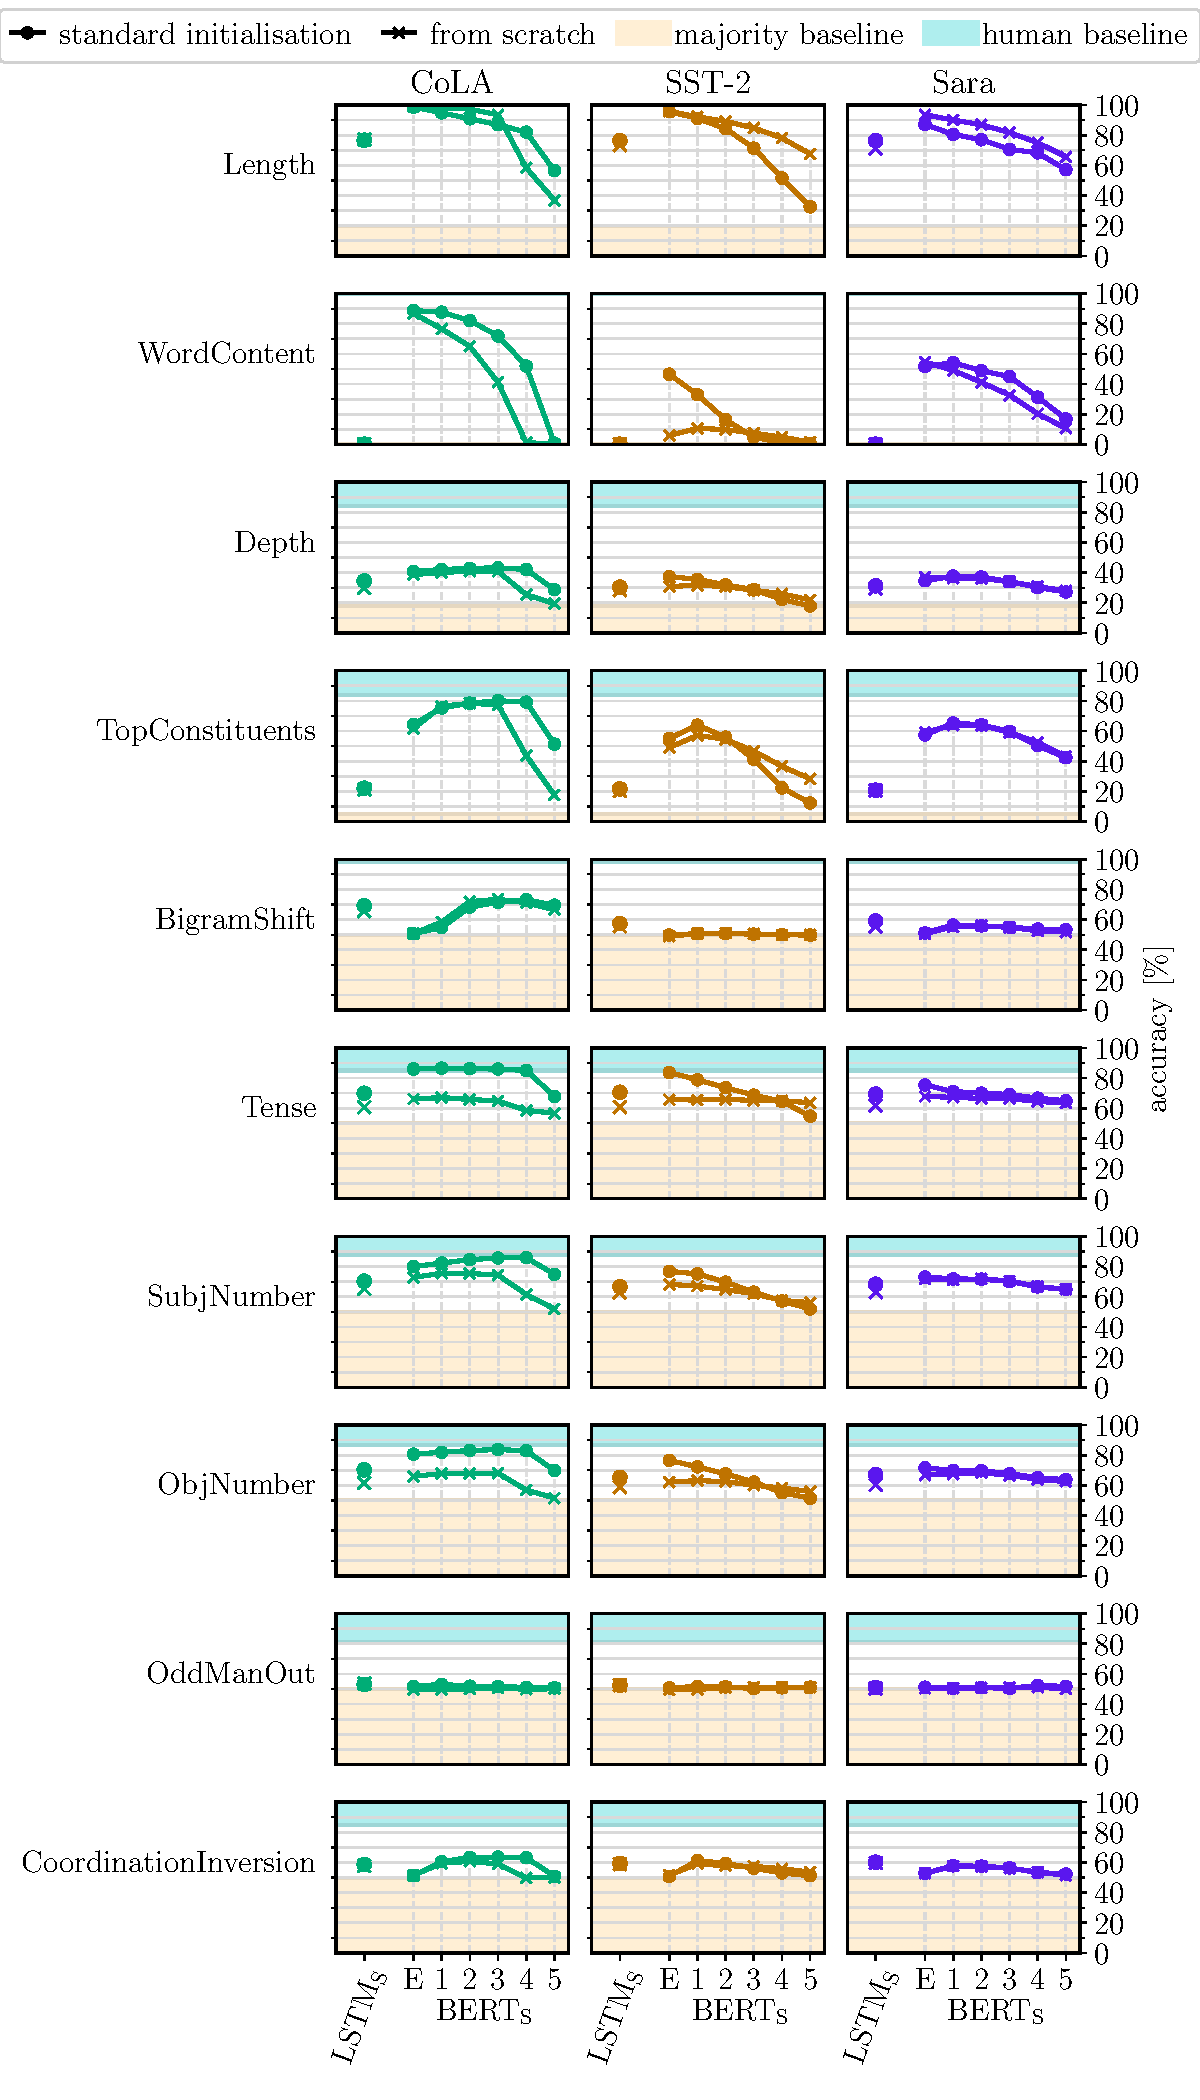
\includegraphics[width=13.5cm]{../experiments/analysis/img/probing_students_scratch.pdf}}
    \caption{Probing results comparing studentss initialised in the standard way (with embeddings from word2vec) with students initialised randomly and trained from scratch. Bounding the expected model performance from below and from above are again the majority-class baseline and the human performance baseline, as reported by \citet{Conneau_2018}.}
    \label{fig:probing-students-scratch}
  \end{figure}
}

\end{document}
